% ========================================= TEMPLATE INFO ========================================
%
% Author:       P4ntomime
% Version:      1.0.0
% Last updated: 2024-02-18
% Brief:        A LaTeX template for summaries. See README.md for more information.
% 
% ================================================================================================
\documentclass[8pt, a4paper, twoside]{extarticle}
% Font size:    8pt
% Paper size:   A4
% style:        twoside (needed, so odd and even pages have different margins)
% orientation:  portrait. (use 'landscape' for landscape orientation)


% ========================================= DOCUMENT INFO =========================================
\def\title{Physik 3 -- SWO}                                 % title
\def\shorttitle{Ph3SWO}                                     % short title (displayed as PDF title)
\def\dozent{Prof. Dr. Gregor Dudle}                         % lecturer
\def\semester{HS 2023/2024}                                 % semester
\def\author{Simone Stitz, Yanick Thalmann, Laurin Heitzer}  % author(s)
\def\repo{https://gitlab.com/sstitz/physik-3-swo}           % repository link
\def\version{1.0.\today}                                    % version
\def\pagelimit{40}                                          % page limit -> causes pages after limit to be red
\def\titleoption{compact}                                   % options: compact, normal
\def\enableToC{true}                                        % enables / disables table of contents

% ================================= PACKAGES, SETUP AND COMMANDS ==================================
\input{preamble.tex}


% =========================================== DOCUMENT ============================================
\begin{document}
    \begin{layout}
        \part{Optik}
        \section{Optische Grössen}

\subsection{Licht}

Licht kann auf mehrere Arten beschrieben werden:


\subsubsection{Lichtstrahlen}

\begin{minipage}[t]{0.48\columnwidth}
    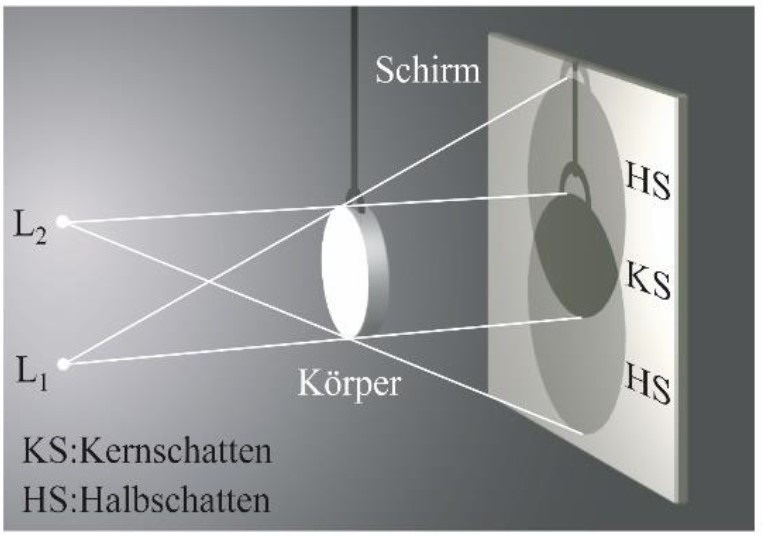
\includegraphics[width=\columnwidth, align=t]{images/lichtstrahlen.jpg}
\end{minipage}
\hfill
\begin{minipage}[t]{0.48\columnwidth}
    Die \textbf{geometrische Optik} oder \textbf{Strahlenoptik} geht davon aus, dass sich das Licht im Vakuum als \textbf{geradliniger Strahl} ausbreitet.

    \medskip

    Mit der geometrischen Optik können die Phänomene Reflexion und Brechung erklärt werden.
\end{minipage}


\subsubsection{Lichtwellen}

\begin{minipage}[t]{0.48\columnwidth}
    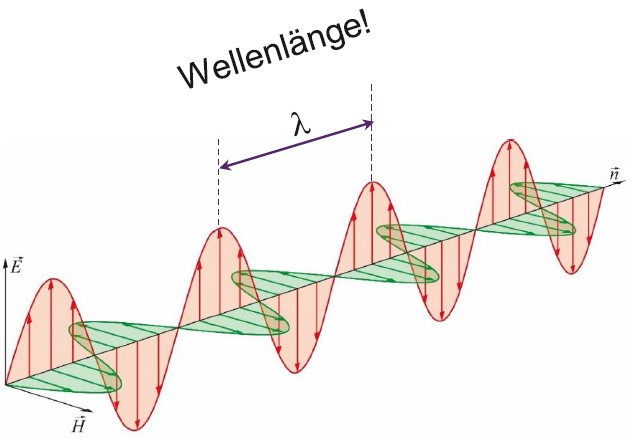
\includegraphics[width=\columnwidth, align=t]{images/lichtwelle.jpg}
\end{minipage}
\hfill
\begin{minipage}[t]{0.48\columnwidth}
    Licht wird als elektromagnetische Welle modelliert.

    \medskip
    
    Bild: linear polarisierte Welle
\end{minipage}


\medskip

\para{Lichtfarben und ihre Frequenzen / Wellenlängen} 

\begin{minipage}[c]{0.42\columnwidth}
    \begin{ctabular}{l c}
        \toprule
        \textbf{Farbe}                          & \textbf{Wellenlänge in $\bm{\nano\meter}$}    \\
        \midrule
        \color{red!50!blue!80!white}violett     & 380 \ldots 435                                \\
        \midrule
        \color{blue}blau                        & 435 \ldots 465                                \\
        \midrule
        \color[HTML]{35c2bd}blaugrün            & 465 \ldots 485                                \\
        \midrule
        \color{green!80!black}grün              & 485 \ldots 565                                \\
        \midrule
        \color{yellow!75!red}gelb               & 565 \ldots 590                                \\
        \midrule
        \color{orange}orange                    & 590 \ldots 630                                \\
        \midrule
        \color{red}rot                          & 630 \ldots 780                                \\
        \bottomrule
    \end{ctabular}
\end{minipage}
\hfill
\begin{minipage}[c]{0.55\columnwidth}
    $$ \boxed{ \lambda = \frac{c}{f} }  \qquad \qquad \qquad \boxed{ \frac{\Delta f}{\Delta \lambda} = \frac{c}{\lambda^2}} $$

    \begin{tabular}{c l c}
        $\lambda$   & Wellenlänge                                       & $[\lambda] = \meter$                          \\
        $c$         & Lichtgeschwindigkeit                              & $[c] = \frac{\meter}{\second}$                \\
                    & $c = 300 \cdot 10^6 \, \frac{\meter}{\second}$    &                                               \\
        $f$         & Frequenz                                          & $[f] = \mathrm{\frac{1}{\second} = \hertz}$ 
    \end{tabular}
\end{minipage}


\subsubsection{Lichtteilchen}

Modellvorstellung des Lichts als ein Fluss von Lichtteilchen (\textbf{Photonen})


$$ \boxed{ E = h \cdot f } $$

\begin{tabular}{c l c}
	$E$ & Energie \textbf{eines} Photons & $[E] = \joule$ \\
	$h$ & Planck'sche Konstante $6.626 \cdot 10^{-34} \frac{\joule}{\hertz}$ & $[h] = \frac{\joule}{\hertz}$ \\
	$f$ & Frequenz & $[f] = \mathrm{\frac{1}{\second} = \hertz}$
\end{tabular}


\subsection{Lichtquellen}

\subsubsection{Thermische Strahler}

\textbf{Schwarzkörper-Modell}: Modell eines Körpers, der in alle Richtungen abstrahlt (und energetisch im Gleichgewicht ist) \\
Ein Schwarzkörper strahlt \textbf{alle} Lichtfarben ab. (auch die für den Mensch nicht sichtbaren.) 

\medskip


\begin{minipage}[t]{0.52\columnwidth}
    \para{Glühbirnen}

    Muss auf allen Wellenlängen angeregt werden, um schliesslich sichtbares Licht abzustrahlen. \\
    \textrightarrow\ Es wird viel Energie nicht nutzbar 'verheizt'
\end{minipage}
\hfill
\begin{minipage}[t]{0.44\columnwidth}
    \para{LEDs}

    Können mit einer bestimmten Frequenz angeregt werden und strahlen nur gewünschtes Licht ab.
    \textrightarrow\ energieeffizient
\end{minipage}



\subsubsection{Lumineszenz}

\begin{minipage}[t]{0.3\columnwidth}
    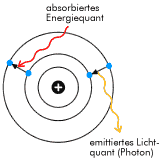
\includegraphics[width=\columnwidth, align=t]{images/lumineszenz.png}
\end{minipage}
\hfill
\begin{minipage}[t]{0.65\columnwidth}
    \begin{itemize}
        \item Elektronen werden angeregt und steigen in energetisch höheren Zustand.
        \item Sobald die Elektronen wieder in ihren Grundzustand zurückkehren wird ein Lichtquant (Photon) abgestrahlt.
        \item Die Leuchtfarbe wird durch die Frequenz der Anregung bestimmt.
    \end{itemize}

    \medskip
    \begin{description}
        \item[Fluoreszenz:] kein Nachleuchten
        \item[Phosphoreszenz:] mit Nachleuchten
    \end{description}
\end{minipage}


\subsection{Messgrössen}

\subsubsection{Radiometrie}

Physikalische Messgrössen der elekromagnetischen Strahlung


\subsubsection{Photometrie}

Radiometrische Grössen, gewichtet mit dem photometrischen Strahlungsäquivalent $K$, welches die \textbf{Empfindlichkeit des menschlichen Auges} angibt.


\paragraph{Photometrischen Strahlungsäquivalent $\bm{K}$}

Gibt die Empfindlichkeit des menschlichen Auges wieder und ist eine empirisch genormte Kurve \\
\textrightarrow\ Menschliches Auge ist bei Wellenlänge von $555 \, \nano\meter$  (grüne Farbe) am empfindlichsten \\
\textrightarrow\ Entspricht $638 \, \frac{\lumen}{\watt}$


\subsection{Gegenüberstellung: Radiometrie -- Photometrie}

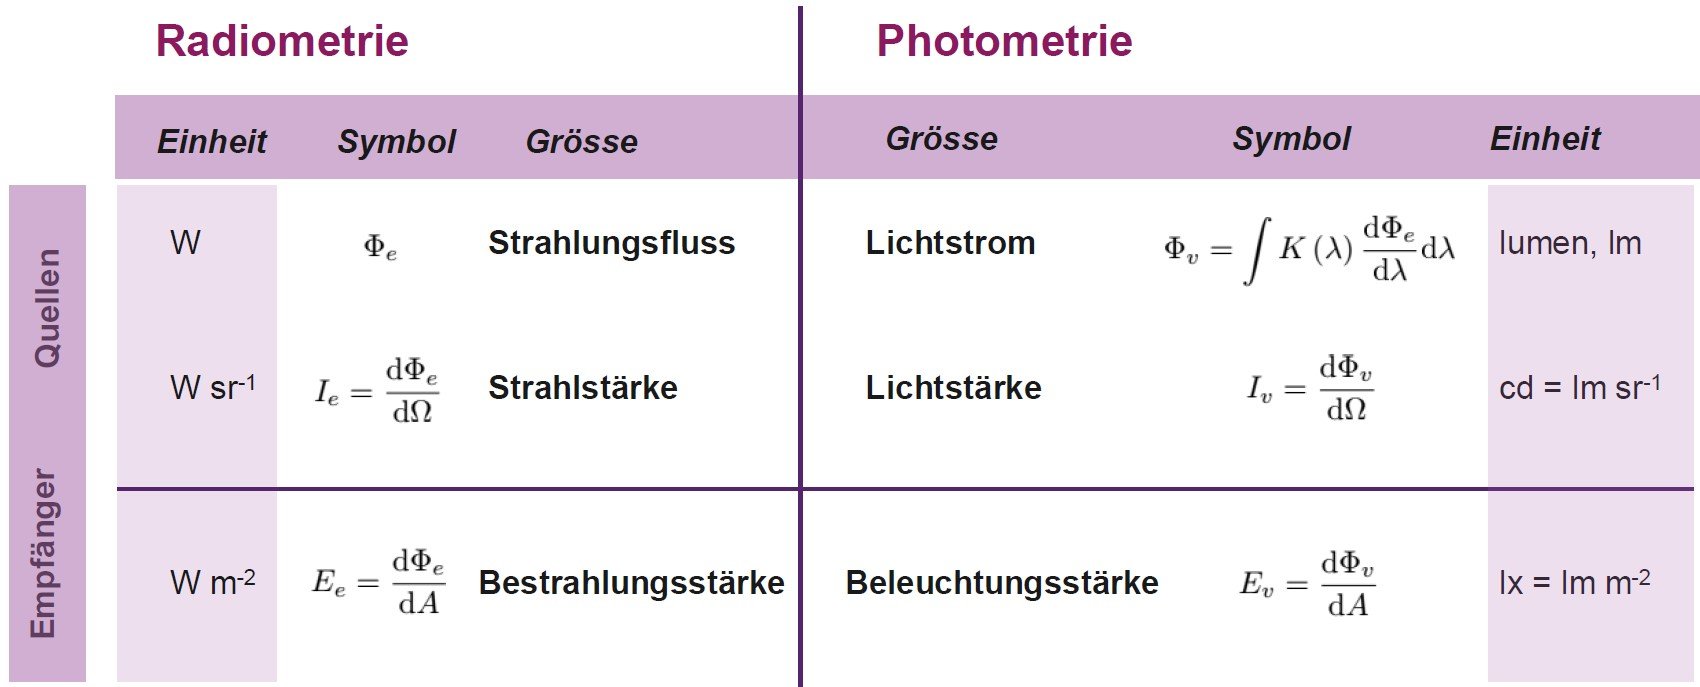
\includegraphics[width=\columnwidth]{images/radiometrie_photometrie.jpg}


\subsection{Raumwinkel}

\subsubsection{Winkel in der Ebene}

\begin{minipage}[t]{0.35\columnwidth}
    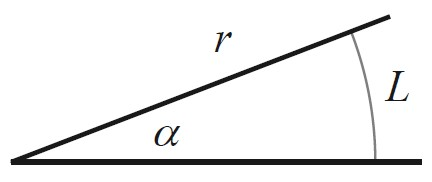
\includegraphics[width=\columnwidth, align=t]{images/winkel_ebene.jpg}
\end{minipage}
\hfill
\begin{minipage}[t]{0.6\columnwidth}
    Länge des Bogens auf einem Kreis mit $r = 1 \, \meter$ 

    \medskip

    \begin{minipage}[c]{0.48\columnwidth}
        $$ \boxed{ \alpha = \frac{L}{r}  } $$ 
    \end{minipage}
    \hfill
    \begin{minipage}[c]{0.48\columnwidth}
        Vollkreis: $2 \, \pi$\\
        $[\alpha] = \rad$ 
    \end{minipage}
\end{minipage}


\subsubsection{Winkel im Raum}

\begin{minipage}[t]{0.3\columnwidth}
    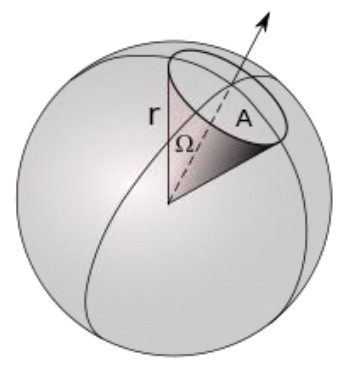
\includegraphics[width=\columnwidth, align=t]{images/winkel_raum.jpg}
\end{minipage}
\hfill
\begin{minipage}[t]{0.66\columnwidth}
    Aufgespannte Fläche, projiziert auf eine Kugel mit $r = 1 \, \meter$
    
    \medskip

    \begin{minipage}[c]{0.48\columnwidth}
        $$ \boxed{ \Omega = \frac{A}{r^2} = \frac{A}{1 \, \meter\squared} } $$
    \end{minipage}
    \hfill
    \begin{minipage}[c]{0.48\columnwidth}
        Kugel: $4 \, \pi$ \\
        $[\Omega] = \steradian$ (Steradiant) 
    \end{minipage}
\end{minipage}


        \section{Reflexion}

\subsection{Reflexionsgesetz}

\begin{minipage}[c]{0.42\columnwidth}
    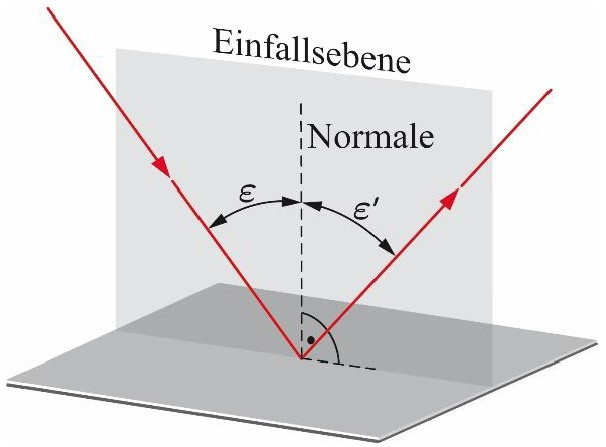
\includegraphics[width=\columnwidth]{images/reflexionsgesetz.jpg}
\end{minipage}
\hfill
\begin{minipage}[c]{0.48\columnwidth}
    \begin{center}
        Einfallswinkel = Ausfallswinkel 
    \end{center}
    $$ \boxed{ \varepsilon = \varepsilon' } $$
\end{minipage}


\subsubsection{Grenzflächen von Reflexionen}

\begin{minipage}{0.4\columnwidth}
    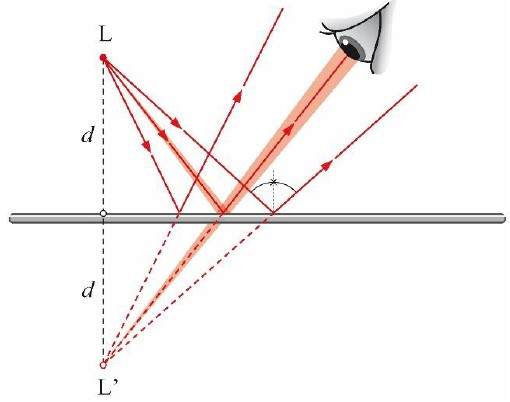
\includegraphics[width=\columnwidth]{images/reflexion.jpg}
\end{minipage}
\hfill
\begin{minipage}{0.58\columnwidth}
    \begin{tabularx}{\columnwidth}{l X}
    $L$ & reelles Bild \\
        & Bild, welches auf Schirm abgebildet werden kann \\
        & \\
    $L'$& virtuelles Bild (Spiegelbild von $L$)\\
        & Bild, welches nicht auf Schirm abgebildet werden kann 
    \end{tabularx}
\end{minipage}

\begin{description}
    \item[Glatter Spiegel:] direkte Reflexion (siehe Bild oben)
    \item[Rauer Spiegel:] diffuse Refelxion
\end{description}



\subsection{Reflexionen -- Spezialfälle}

\begin{tabularx}{\columnwidth}{l X}
    Brennpunkt $F$  & Brennpunkt (Fokus) ist der Punkt, in dem parallel zur optischen Achse auf einen Spiegel oder eine Linse einfallende Stahlen sich schneiden    \\
                    &                                                                                                                                               \\
    Brennweite $f$  & Abstand des Brennpunktes von der Linse bzw. dem Spiegel
\end{tabularx}


\subsubsection{Parabolspiegel}

Parallel einfallende Strahlen werden in einem Punkt fokussiert.

\medskip

\begin{minipage}[c]{0.8\columnwidth}
    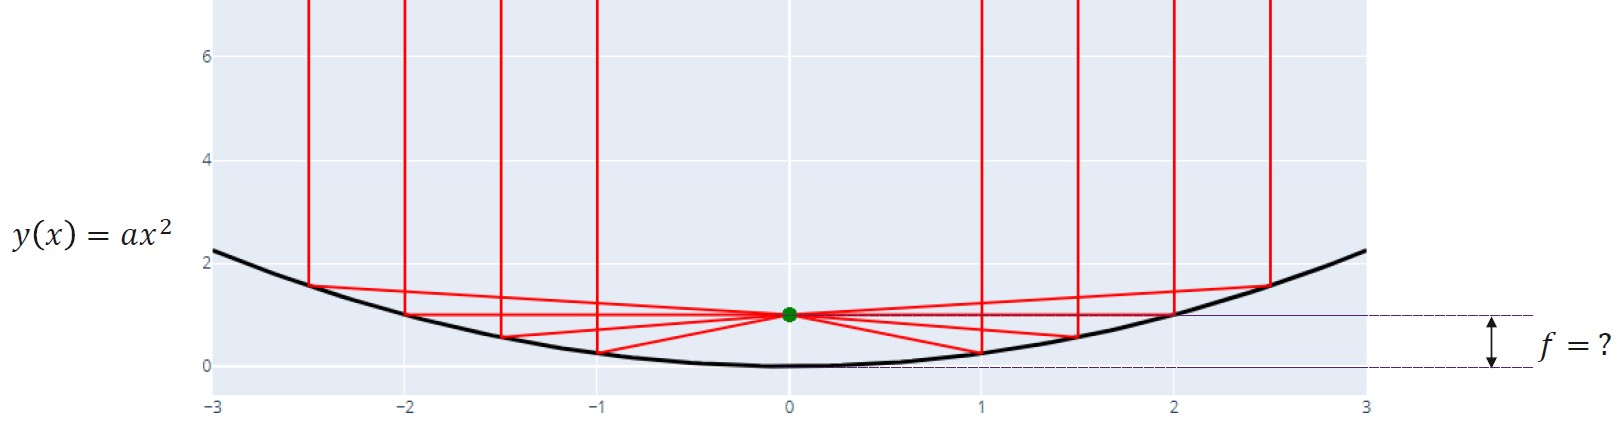
\includegraphics[width=\columnwidth]{images/parabolspiegel.jpg}
\end{minipage}
\hfill
\begin{minipage}[c]{0.18\columnwidth}
    $$ \boxed{ y(x) = a \, x^2 }$$ 
    $$ \boxed{ f = \frac{1}{4 \, a} } $$ 
\end{minipage}


\subsubsection{Elliptischer Spiegel}

Konzentration von Energie in einem nicht zugänglichen Punkt 

\begin{minipage}[t]{0.48\columnwidth}
    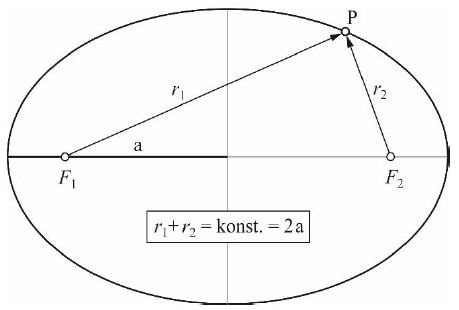
\includegraphics[width=\columnwidth, align=t]{images/elliptischer_spiegel.jpg}
\end{minipage}
\hfill
\begin{minipage}[t]{0.48\columnwidth}
    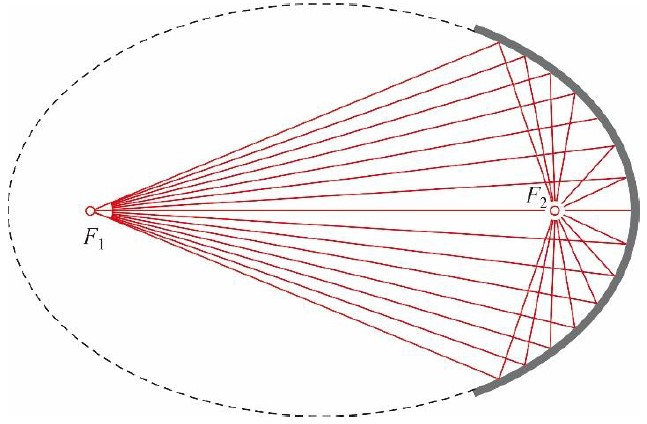
\includegraphics[width=\columnwidth, align=t]{images/elliptischer_spiegel_2.jpg} 
\end{minipage}

$$ \boxed{ y(x) = \frac{x^2}{a^2} + \frac{y^2}{b^2} } $$


\subsubsection{Hyperbolischer Spiegel}

Objekt in Spiegel versetzen 

\begin{minipage}{0.4\columnwidth}
    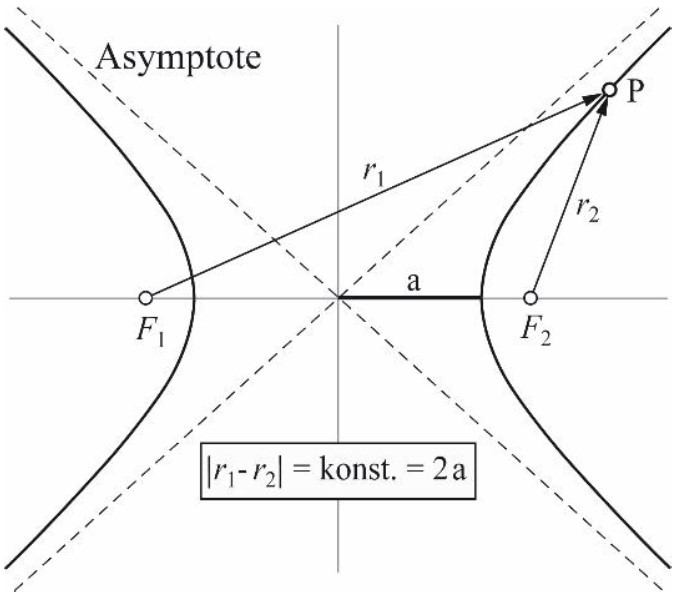
\includegraphics[width=\columnwidth]{images/hyperbolischer_spiegel.jpg} 
\end{minipage}
\hfill
\begin{minipage}{0.48\columnwidth}
    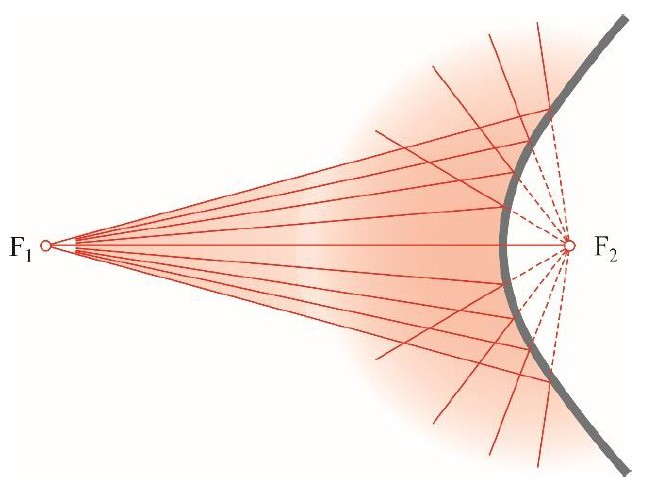
\includegraphics[width=\columnwidth]{images/hyperbolischer_spiegel_2.jpg} 
\end{minipage}

$$ \boxed{ \frac{x^2}{a^2} - \frac{y^2}{b^2} = 1} $$


\subsubsection{Sphärische Spiegel}

Parallel einfallende Stahlen werden nicht mehr in einem Punkt fokussiert (Katakaustik) 

\smallskip

Da die achsnahen Strahlen nach der Reflexion annähernd durch einen Punkt gehen, wird dieser Punkt wieder Brennpunkt $F$ genannt.

\begin{center}
    \begin{minipage}{0.4\columnwidth}
        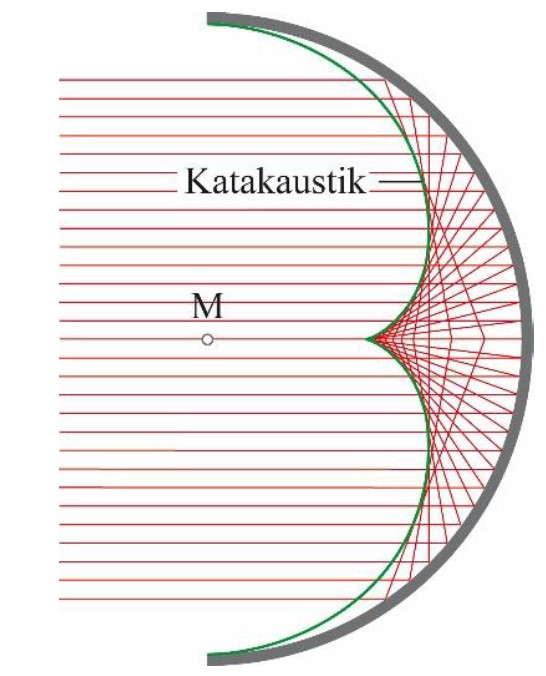
\includegraphics[height=3.5cm]{images/sphaerischer_spiegel_2.jpg}
    \end{minipage}
    \begin{minipage}{0.45\columnwidth}
        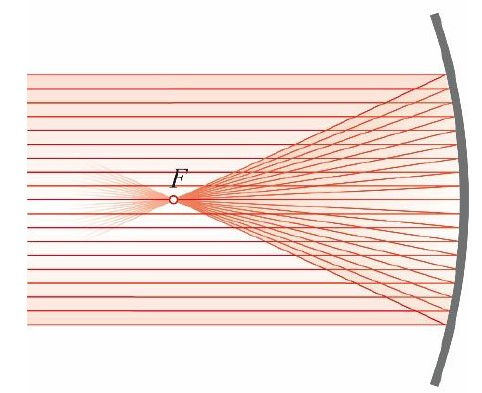
\includegraphics[height=3.5cm]{images/sphaerischer_spiegel.jpg}
    \end{minipage}
\end{center}

\vspace{-0.3cm}

\begin{minipage}[c]{0.2\columnwidth}
    $$ \boxed{ f = \frac{r}{2} } $$
    \smallskip
\end{minipage}
\hfill
\begin{minipage}[c]{0.76\columnwidth}
    \begin{tabular}{clc}
        $f$ & Brennweite                    & $[f] = \meter$    \\
        $r$ & Krümmungsradius des Spiegels  & $[r] = \meter$    \\
    \end{tabular}
\end{minipage}

\vspace{-0.3cm}


        \section{Brechung}

Fällt ein Lichtstrahl auf die Grenzfläche zweier Medien, so dringt ein Teil des einfallenden Lichtes in das zweite Medium ein. \\
Die auftrentende Richtungsänderung wird als \textbf{Brechung} bezeichnet. \\
Der in das zweite Medium eindringende Strahl wird \textbf{gebrochener Strahl} genannt.


\subsection{Brechungsgesetz / Geschwindigkeit}

\begin{minipage}[t]{0.34\columnwidth}
    \textbf{Achtung:} Es gilt $n_1 < n_2$

    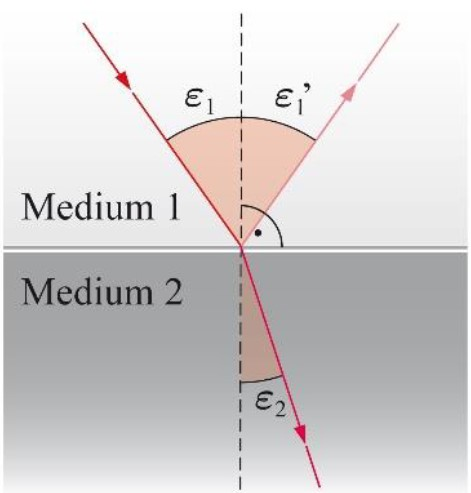
\includegraphics[width=\columnwidth, align=t]{images/brechung.jpg}
\end{minipage}
\hfill
\begin{minipage}[t]{0.64\columnwidth}
    $$ \boxed{ \frac{\sin(\varepsilon_1)}{\sin(\varepsilon_2)} = \frac{n_2}{n_1}  } \qquad \qquad
    \boxed{ v_i = \frac{c}{n_i}  } $$

    Je grösser $n$, desto grösser die Ablenkung und desto\\
    kleiner $\varepsilon$

    \medskip

    \begin{tabular}{@{}c l c@{}}
        $\varepsilon_i$ & Winkel zur Normalen & $[\varepsilon_i] = \degree$ \\
        $n_i$ & Brechungsindex & $[n_i] = 1$ \\
        $v_i$ & Geschwindigkeit im Medium $n_i$ & $[v_i] = \frac{\meter}{\second}$ \\
        $c$ & Lichtgeschwindigkeit $c = 300 \cdot 10^6 \, \frac{\meter}{\second}$ & $[c] = \frac{\meter}{\second}$
    \end{tabular}
\end{minipage}


\medskip

\paragraph{Anwendung: Glasfaser}

Der Lichtstrahl bliebt in der Kernzone (Medium 1) gefangen, da diese einen grösseren Brechungsindex hat als die Mantelschicht (Medium 2)
\begin{center}
    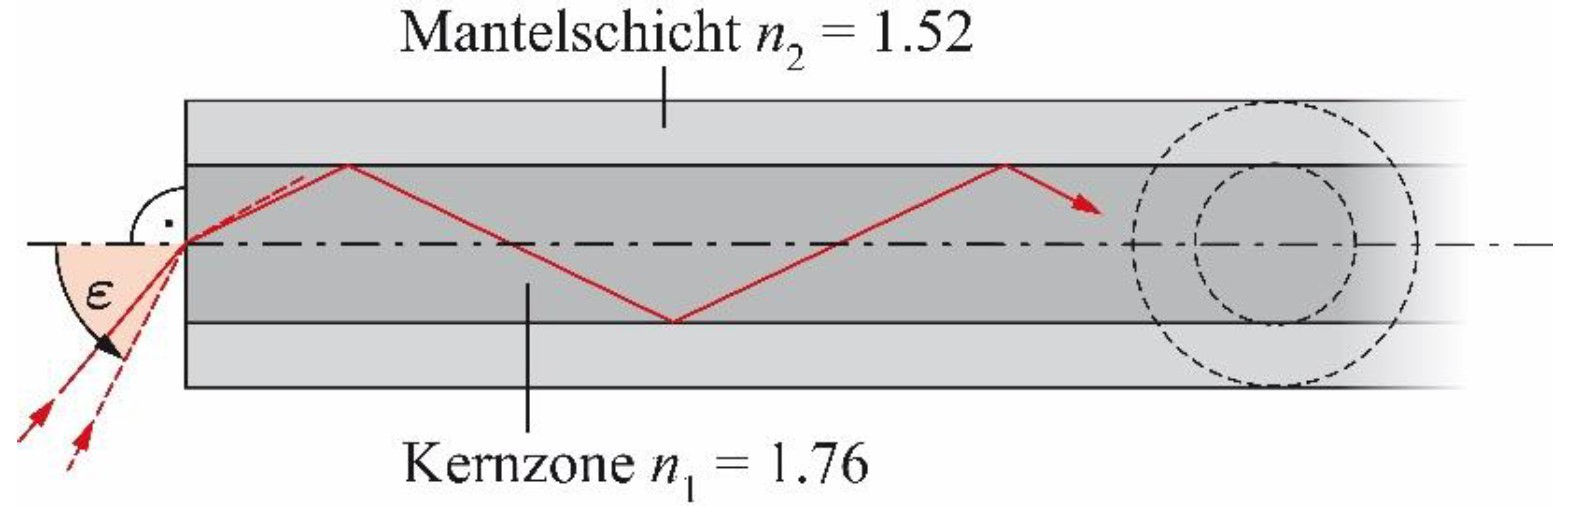
\includegraphics[width=0.75\columnwidth]{images/glasfaser.jpg}
\end{center}



\subsection{Totalreflexion}

\begin{minipage}[c]{0.6\columnwidth}
    Der Einfallswinkel $\varepsilon_1$ kann nicht grösser als 90° sein. \\
    Für $\varepsilon_1 = 90$° berechnet sich $\varepsilon_2 = \varepsilon_g$ aus: 
\end{minipage}
\hfill
\begin{minipage}[c]{0.38\columnwidth}
    $$ \varepsilon_g = \arcsin \left( \frac{n_1}{n_2} \right) $$
\end{minipage}

\smallskip

Für den Grenzfall von $\varepsilon_1 > 90$° wird der gesamte Stahl reflektiert.

\begin{center}
    \begin{minipage}{0.4\columnwidth}
        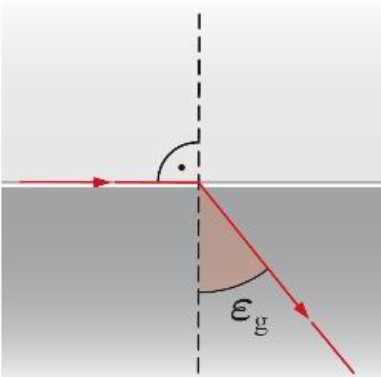
\includegraphics[height=3.5cm]{images/totalreflexion.jpg}
    \end{minipage}
    \begin{minipage}{0.4\columnwidth}
        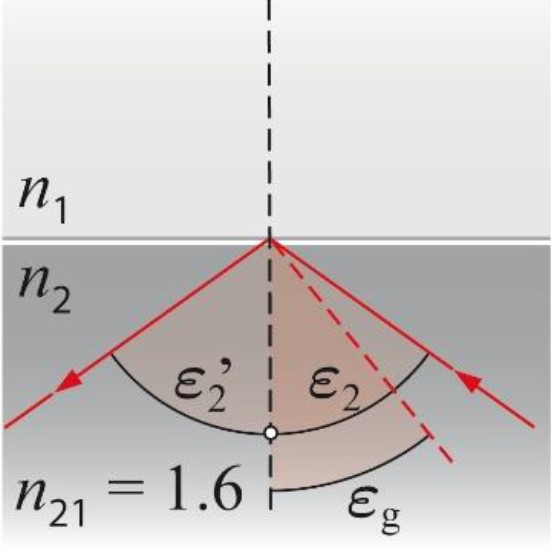
\includegraphics[height=3.5cm]{images/totalreflexion_2.jpg}
    \end{minipage}
\end{center}



\subsection{Brechung an ebenen Grenzflächen}

Ein Lichtstrahl wird verschoben bzw. in eine beliebige Richtung geändert

\begin{minipage}{0.32\columnwidth}
    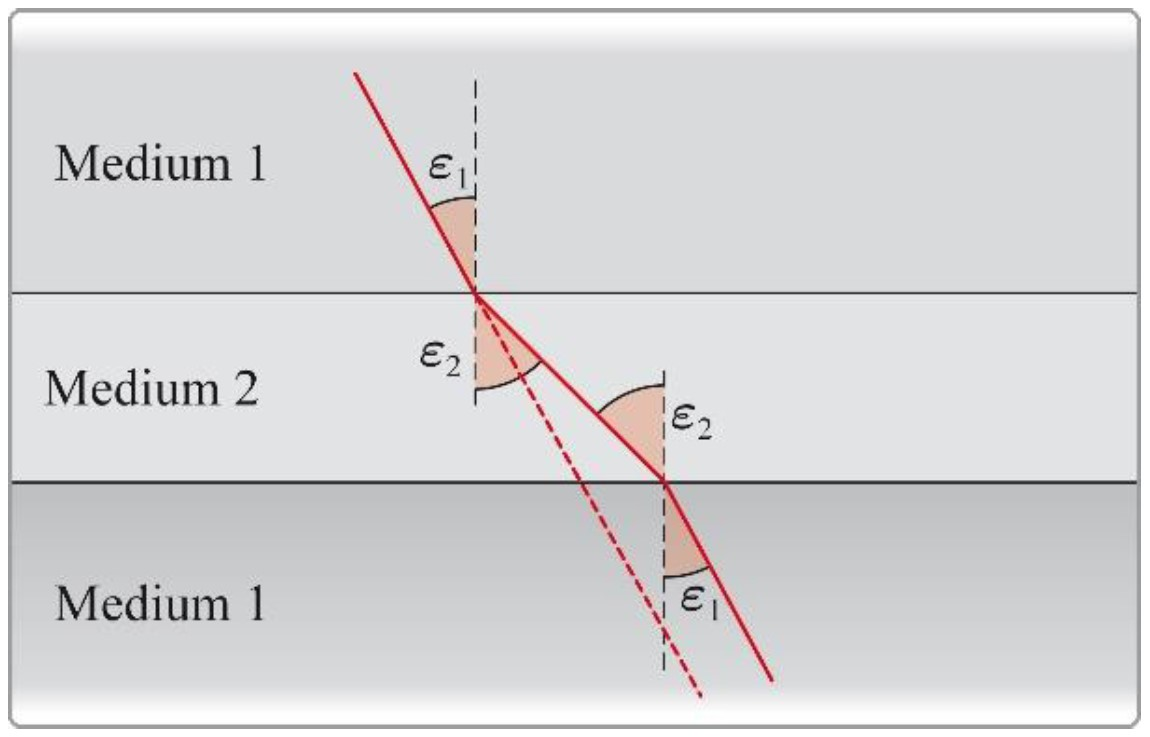
\includegraphics[width=\columnwidth]{images/verschiebung_lichtstrahl.jpg}
\end{minipage}
\hfill
\begin{minipage}{0.35\columnwidth}
    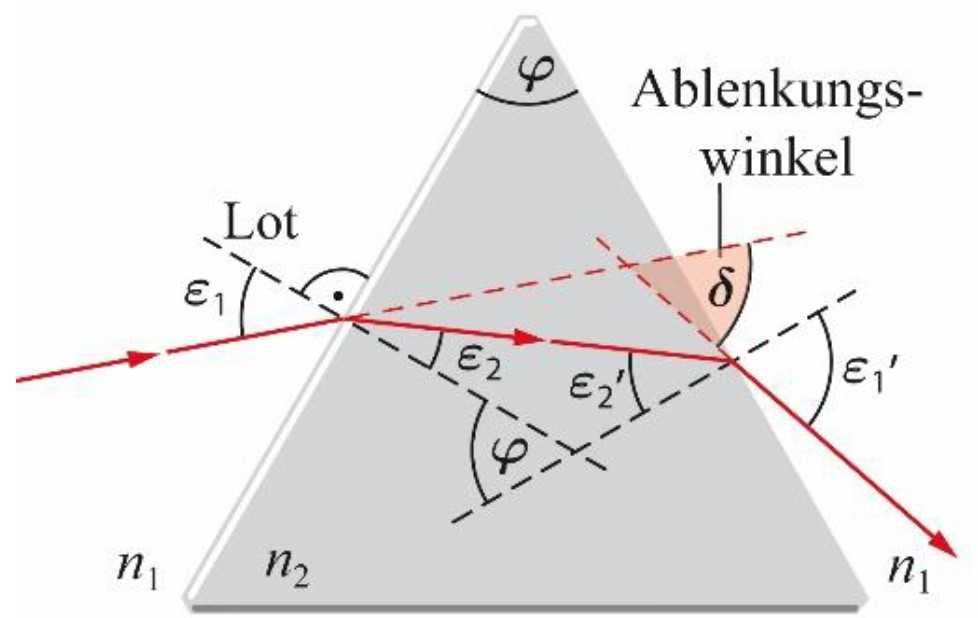
\includegraphics[width=\columnwidth]{images/prisma.jpg}
\end{minipage}
\hfill
\begin{minipage}{0.3\columnwidth}
    $$\boxed{ n = \frac{\sin (\varepsilon_1)}{\sin(\varepsilon_2)} = \frac{\sin \left(\frac{\varphi + \delta}{2} \right)}{\sin \left( \frac{\varphi}{2} \right)} } $$
\end{minipage}


\subsection{Brechung an gekrümmten Flächen}

Die Anwendung der Brechung ist eine Linse.

\medskip

\paragraph{Linsentypen}

\begin{minipage}{0.3\columnwidth}
    \centering
    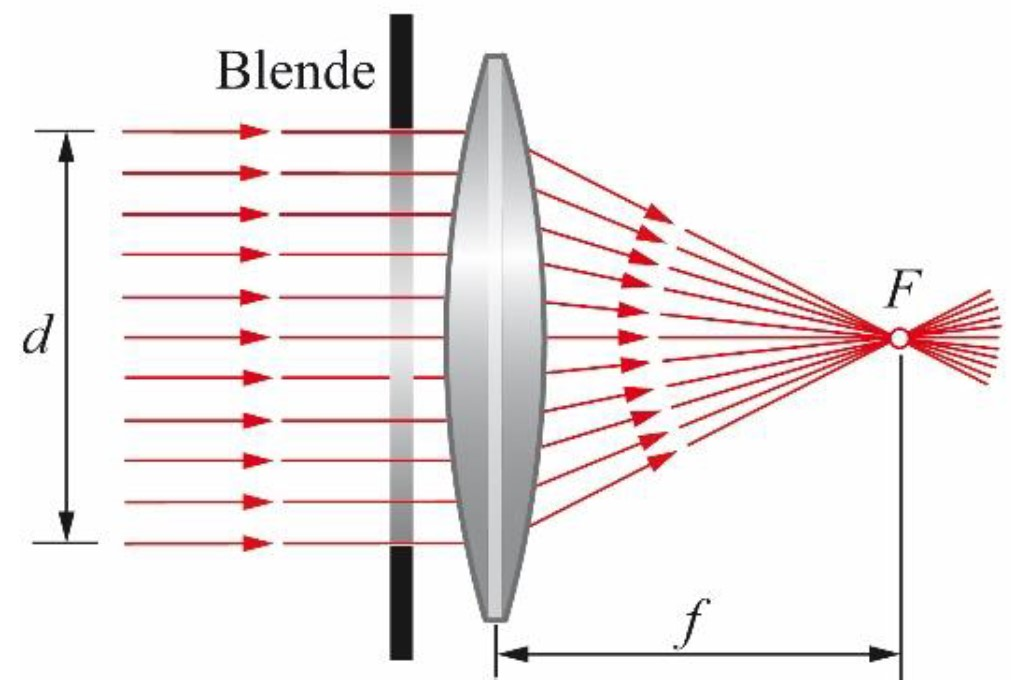
\includegraphics[height=2.0cm]{images/sammellinse.jpg}\\
    Sammellinse
\end{minipage}\hfill
\begin{minipage}{0.3\columnwidth}
    \centering
    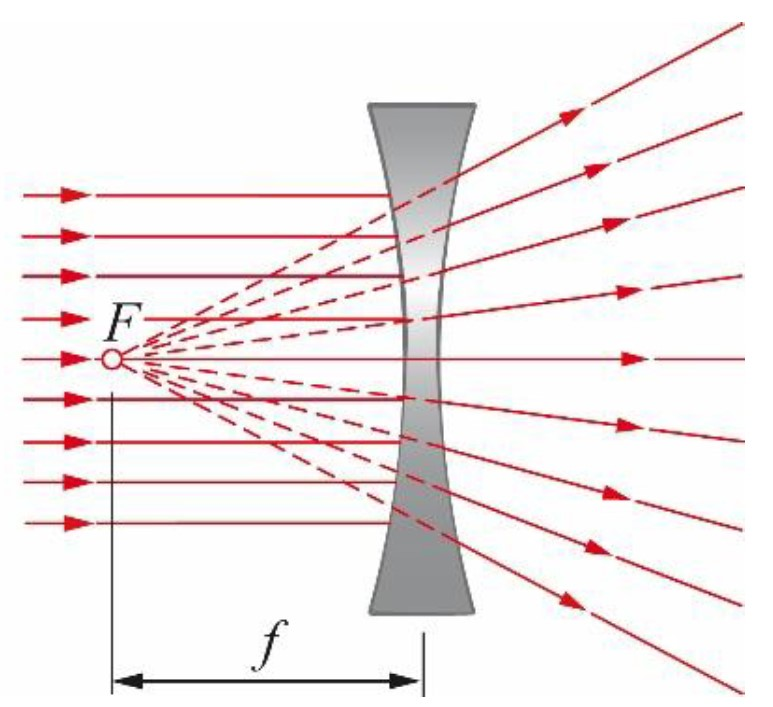
\includegraphics[height=2.0cm]{images/zerstreuungslinse.jpg}\\
    Zerstreuungslinse
\end{minipage}\hfill
\begin{minipage}{0.3\columnwidth}
    \centering
    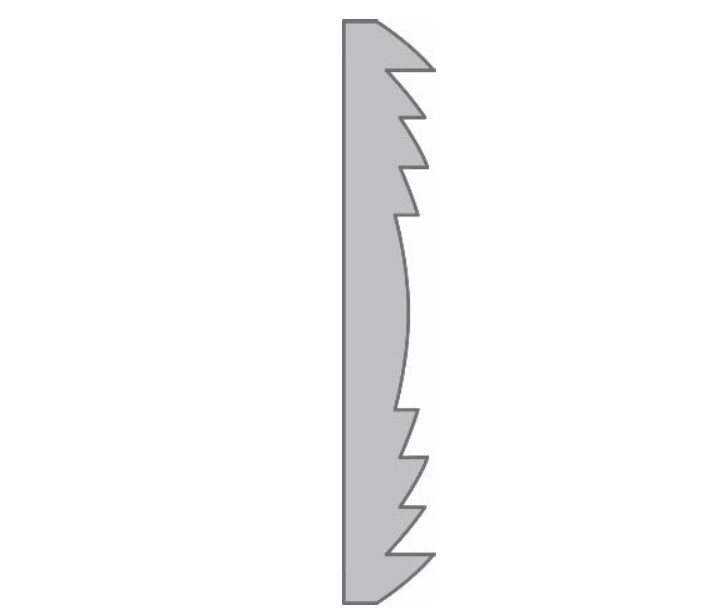
\includegraphics[height=2.0cm]{images/fresnellinse}\\
    Fresnellinse
\end{minipage}

\medskip
\textbf{Fresnellinse:} Es kann vermieden werden, dass die Linse eine übermässige Dicke aufweist. 


\example{Brechung mit  zwei Linsen}

\begin{center}
    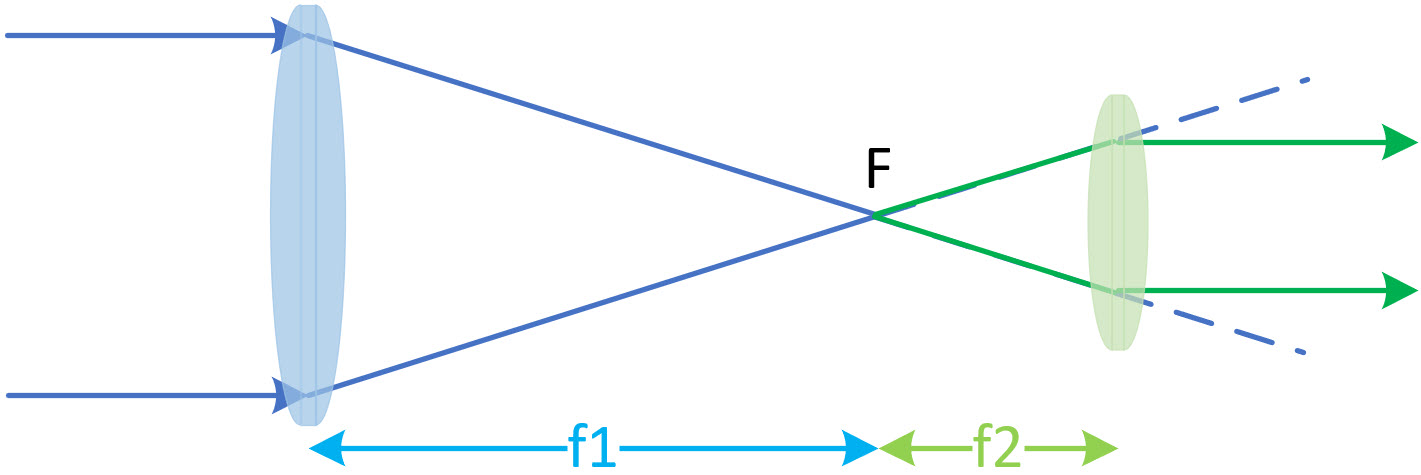
\includegraphics[width=0.85\columnwidth]{images/linsen.jpg}
\end{center}
Rechts gibt es ein kleineres Bild als links.


\subsection{Dispersion}\label{Dispersion Optik}

Der \textbf{Brechungsindex} eines Mediums ist eine \textbf{Funktion der Wellenlänge:} $n = n(\lambda)$ \\
Diese Wellenlängenabhängigkeit wird als \textbf{Dispersion} bezeichnet.
\[
    \boxed{ n^2(\lambda) = 1 + \frac{A}{ \frac{1}{\lambda_0^2} -  \frac{1}{\lambda^2} } }   \qquad \qquad
    \boxed{ n^2(f) = 1 + \frac{A'}{f_0^2 - f^2} }
\]


\subsubsection{Abbe Zahl $\bm{V}$}

Gibt an, wie stark dispersiv ein Material ist \\
Grosse Abbe-Zahl \textrightarrow\ wenig dispersives Material

        \section{Abbildungen -- Linsen}

\subsection{Konstruktions-Anweisung}

Man benutzt zwei der drei Hauptstrahlen:

\begin{ctabular}{l l >{\textrightarrow}c l}
    1. & Parallel Strahl & & Brennpunkt \\
    2. & Mittelpunkt Strahl & & mit gleichem Winkel zurück \\
    3. & Brennpunkt Strahl & & Paralleler Strahl
\end{ctabular}

\begin{minipage}{0.48\columnwidth}
    \centering
    \textbf{Reelles Bild}

    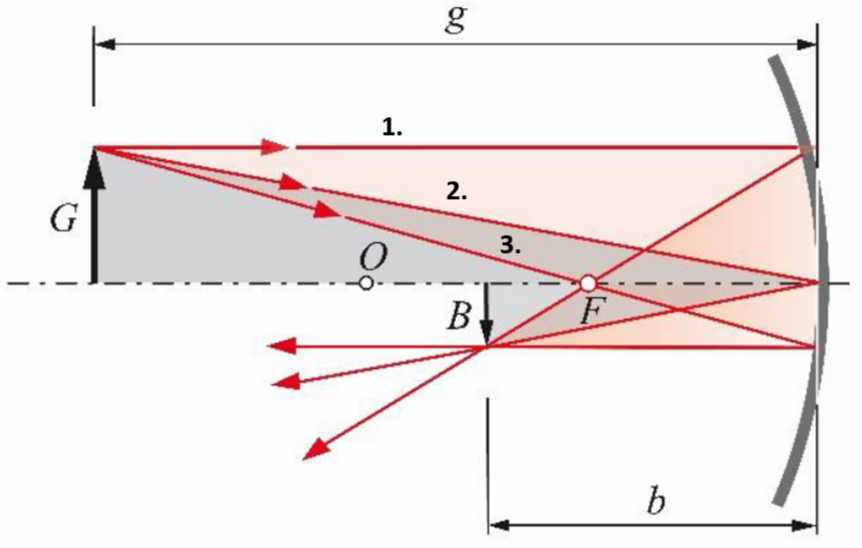
\includegraphics[width= 0.9\columnwidth]{images/reelles_bild.png}
\end{minipage}
\hfill
\begin{minipage}{0.48\columnwidth}
    \centering
    \textbf{Virtuelles Bild}

    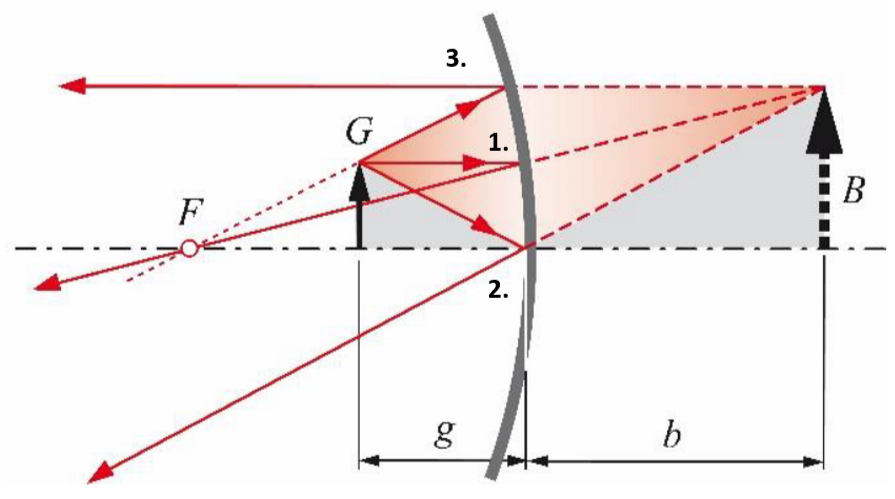
\includegraphics[width= 0.9\columnwidth]{images/virtuelles_bild.png}
\end{minipage}

$B$ wird als \textbf{reeller Bildpunkt} bezeichnet, wenn sich die austretenden Strahlen schneiden.

\smallskip
$B$ wird als \textbf{virtueller Bildpunkt} bezeichnet, wenn sich nur die Verlängerungen der austretenden Strahlen schneiden. 


\subsubsection{Terminologie}

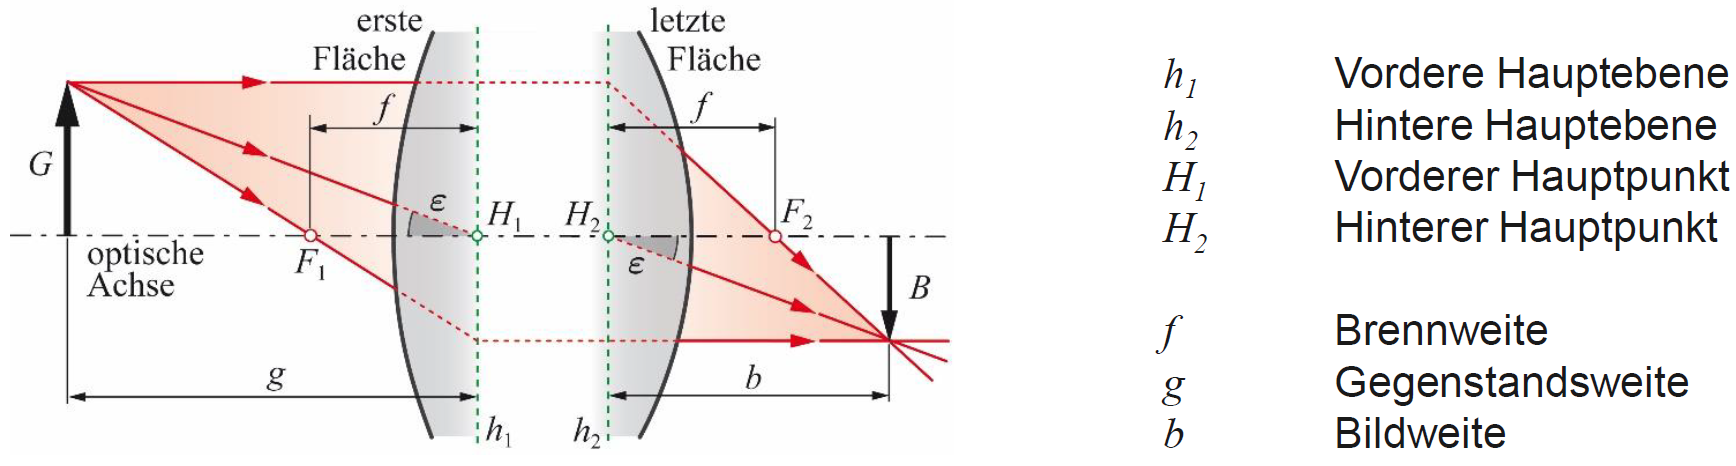
\includegraphics[width=0.9\columnwidth]{images/terminologie.png}

Die \textbf{Öffnungsblende} oder \textbf{Aperturblende} bergrenz das in das System einfallende Lichtbündel

\smallskip
Die \textbf{Feldblende} begrenzt das Bildfeld. Sie legt den Ausschnitt der Objektebene fest, der abgebildet wird.


\example{Abbildungen bei zwei Sammellinsen}

\begin{minipage}{0.48\columnwidth}
    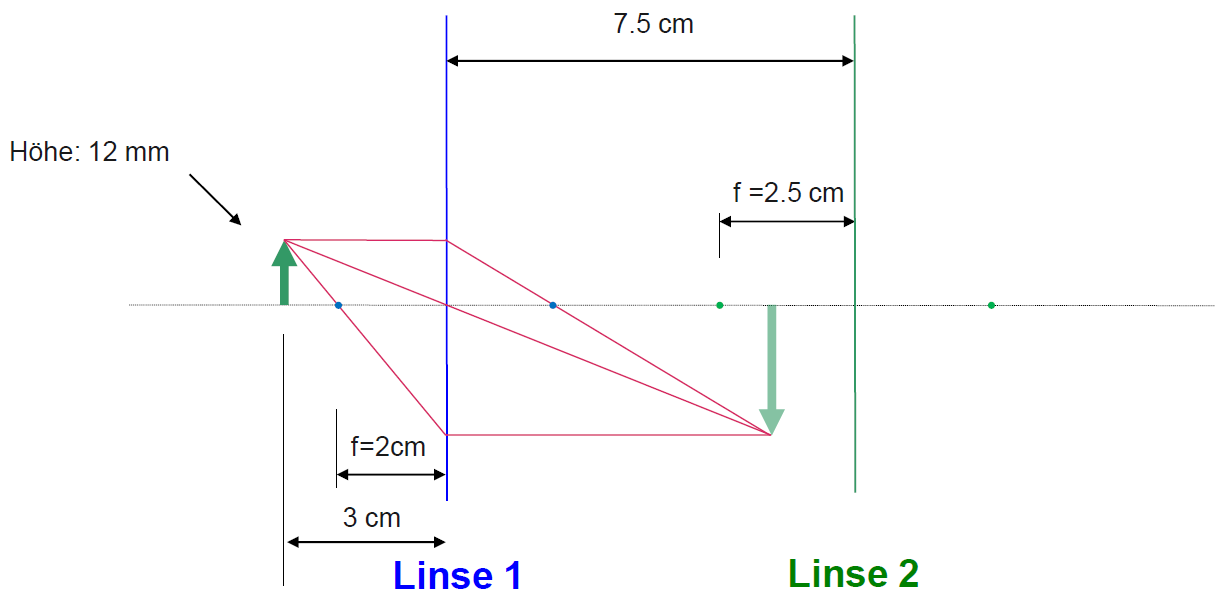
\includegraphics[width=\columnwidth]{images/zwei_sammellinsen_1.png}
\end{minipage}
\hfill
\begin{minipage}{0.48\columnwidth}
    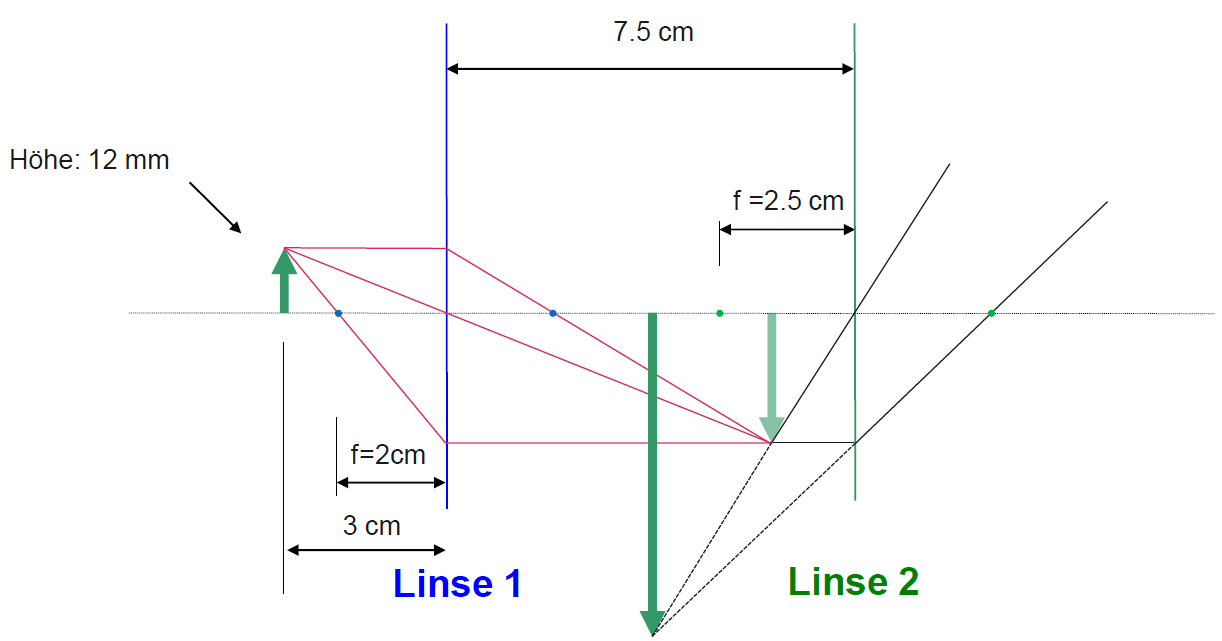
\includegraphics[width=\columnwidth]{images/zwei_sammellinsen_2.png}
\end{minipage}


\subsection{Abbildungsgleichungen}

\textbf{Ein Bild ist scharf dargestellt, wenn die Abbildungsgleichung erfüllt ist!}

\medskip

\begin{minipage}{0.48\columnwidth}
    \paragraph{Abbildungsgleichung}
    $$ \boxed{ \frac{1}{b} + \frac{1}{g} = \frac{1}{f} } $$
\end{minipage}
\hfill
\begin{minipage}{0.48\columnwidth}
    \paragraph{Newtonsche Abb.-Gleichung}
    $$ \boxed{ x_b \cdot x_g = f^2 } $$
\end{minipage}

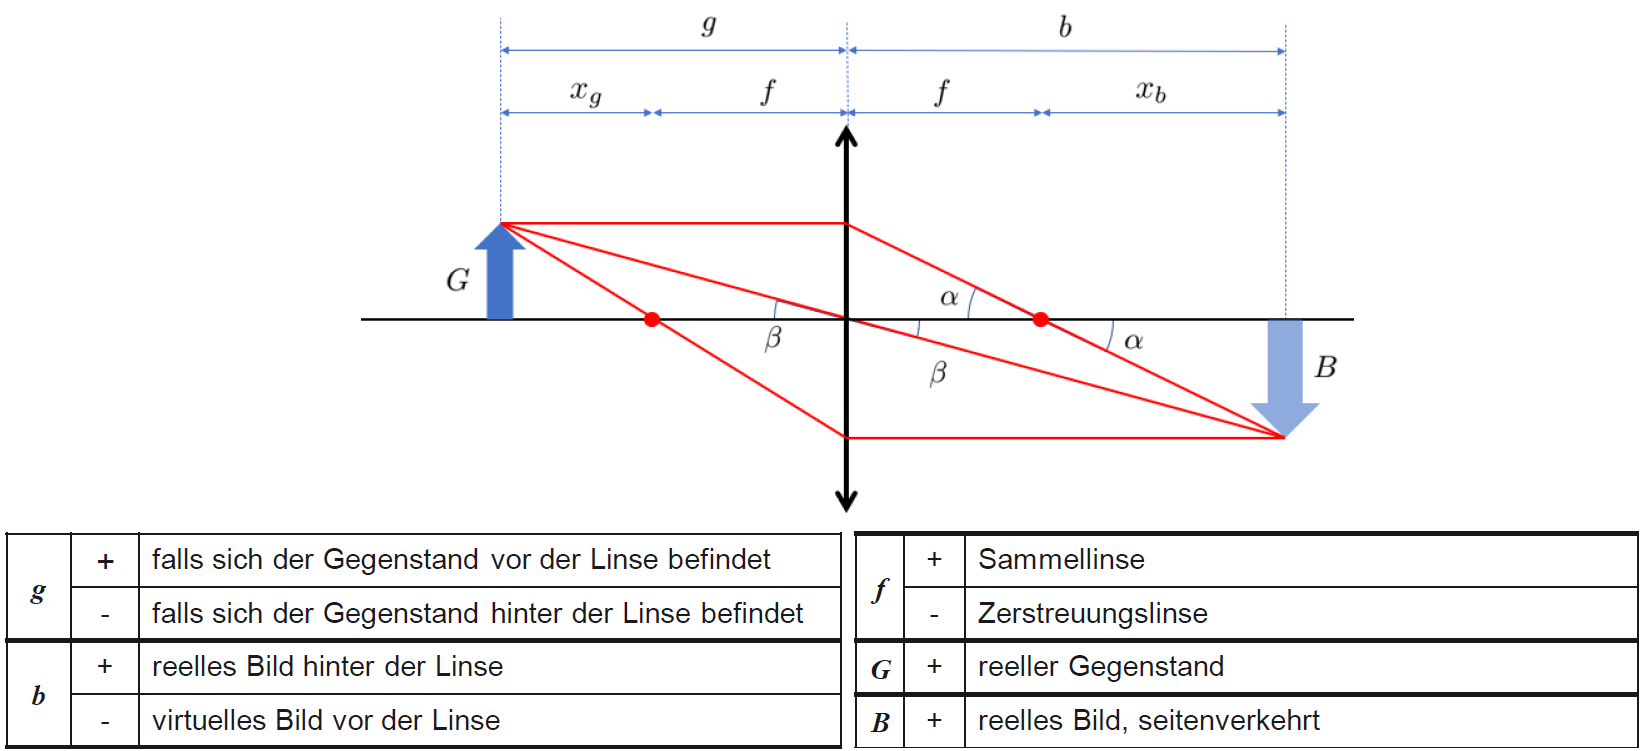
\includegraphics[width=\columnwidth]{images/abbildungsgleichung.png}



\textcolor{blue}{\textbf{Hinweis:} Ein Spiegel hat eine Brennweite von $f = \infty$ \\
\textrightarrow\  Vereinfachung der Abbildungsgleichung!}


\subsubsection{Vergrösserungsverhältnis}

\begin{minipage}{0.35\columnwidth}
    $$ \boxed{ V = \frac{B}{G} = \frac{b}{g} } $$
    $$ \boxed{ V_{\rm tot} = V_1 \cdot V_2 } $$ 
\end{minipage}
\hfill
\begin{minipage}{0.6\columnwidth}
    \begin{tabular}{c l c}
        $V$ & Vergrösserungsverhältnis  & $[V] = 1$         \\
        $b$ & Bildweite                 & $[b] = \meter$    \\
        $g$ & Gegenstandsweite          & $[g] = \meter$    \\
        $B$ & Bildgrösse                & $[B] = \meter$    \\
        $G$ & Gegenstandsgrösse         & $[G] = \meter$    \\
        $f$ & Brennweite                & $[f] = \meter$ 
    \end{tabular}
\end{minipage}



\subsection[Brechkraft]{Brechkraft $\bm{D}$}

\begin{minipage}[t]{0.65\columnwidth}
    Die Optiker benutzen nicht die Brennweite sondern die Brechkraft in \textbf{Dioptrie}  \\
    Es gilt: $1 \, \mathrm{dpt} = 1 \, \reciprocal\meter$
\end{minipage}
\hfill
\begin{minipage}[t]{0.25\columnwidth}
    $$ \boxed{ D = \frac{1}{f} }$$
\end{minipage}






\subsection{Linsenschleifergleichung}

\begin{minipage}[t]{0.52\columnwidth}
    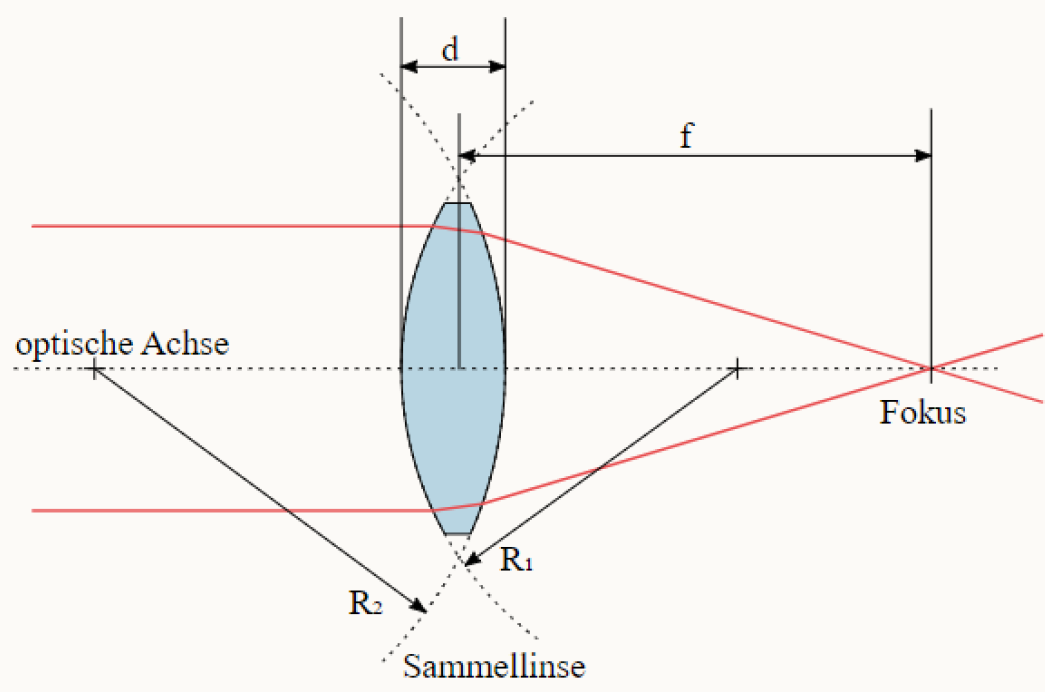
\includegraphics[width=\columnwidth, align=t]{images/Linsenschleifergleichung.png}
\end{minipage}
\hfill
\begin{minipage}[t]{0.46\columnwidth}
    $$\boxed{D = \left( \frac{n_2}{n_1} - 1 \right)  \left(  \frac{1}{R_1} - \frac{1}{R_2} \right) }$$

    \cbl{\textbf{Achtung:} Vorzeichen von $R_i$ beachten!} 

    \raggedright%
    Beide haben gleiches Vorzeichen, wenn Krümmungsmittelpunkte auf gleicher Seite der Linse liegen
\end{minipage}


\subsubsection{Symmetrische Linsen ($\bm{R_1 = R_2}$)}

Für symmetrische Linsen gilt:

\smallskip

\begin{minipage}{0.48\columnwidth}
    $$\boxed{D = (n - 1)\frac{2}{R}}$$
    $$\boxed{f = \frac{1}{D} = \frac{R}{2}\frac{1}{(n - 1)}} $$
\end{minipage}
\hfill
\begin{minipage}{0.48\columnwidth}
    \begin{tabular}{c l c}
        $D$     & Brechkraft        & $[D] = \mathrm{dpt}$                  \\
        $f$     & Brennweite        & $[f] = \frac{1}{\second} = \hertz$    \\
        $R_i$   & Linsenradius      & $[R_i] = \meter$                      \\
        $n$     & Brechungsindex    & $[n] = 1$
    \end{tabular}
\end{minipage}




\subsubsection{Kombination von zwei dünnen Linsen ohne Zwischenraum}

Die Kombination von zwei dünnen Linsen ohne Zwischenraum ist wie folgt definiert:

$$ \boxed{D = D_1 + D_2} $$


\subsection{Konvexe und Konkave Linsen}

\begin{description}
    \item[Konvex:] nach aussen gewölbt \textrightarrow\ Sammellinsen
    \item[Konkav:] nach innen gewölbt \textrightarrow\ Zerstreuungslinsen
\end{description}

\vspace{-0.2cm}

\begin{center}
    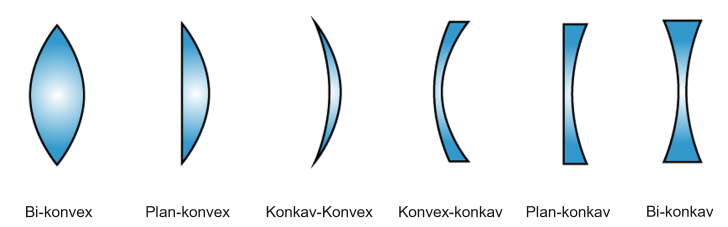
\includegraphics[width=0.9\columnwidth]{images/Konvex.png}
\end{center}

\vspace{-0.2cm}


\subsection{Aberration}

Unter dem Begriff Aberration versteht man die Abweichung vom idealisierten Fall.

\begin{center}
    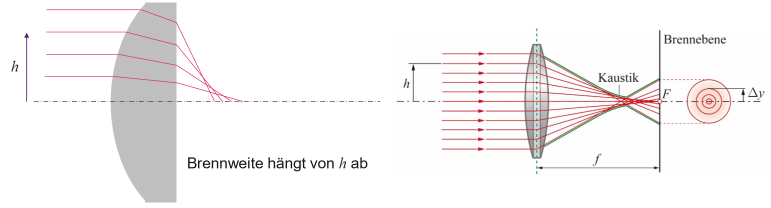
\includegraphics[width=0.9\columnwidth]{images/Aberration.png}
\end{center}



\subsubsection{Astigmatismus}

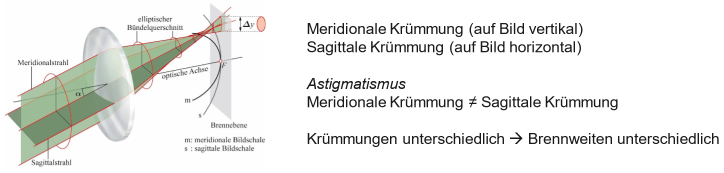
\includegraphics[width=0.9\columnwidth]{images/Astigmatismus.png}


\subsection{Polarisation}

\subsubsection{Lineare Polarisation}

\begin{outline}
    \1 $E_x$ und $E_y$ können \textbf{unterschiedliche Amplituden} haben
    \1 Die \textbf{Phasen müssen gleich} sein.
\end{outline}

\medskip


\begin{minipage}{0.4\columnwidth}
    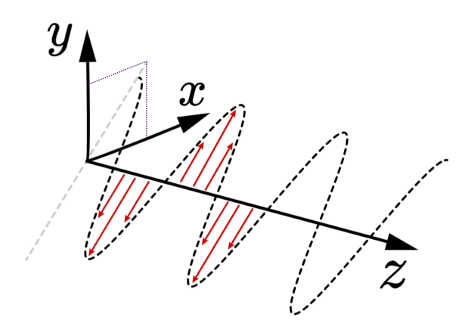
\includegraphics[width=\columnwidth]{images/lineare_Polarisation.png}
\end{minipage}
\hfill
\begin{minipage}{0.58\columnwidth}
    EM-Wellen können mit dem Herzschen Gitter oder mit dem \textbf{Brewster Winkel} linear Polarisiert werden.
    $$ \boxed{  \vec{E} = \begin{pmatrix} E_x \\  E_y \\  0  \end{pmatrix}  } $$
    \begin{center}
        $\vec{E}$ kann zu $\vec{0}$ werden 
    \end{center}
\end{minipage}


\subsubsection{Brewster Winkel}

\begin{minipage}{0.38\columnwidth}
    \textbf{Achtung:} Es gilt $n_1 < n_2$

    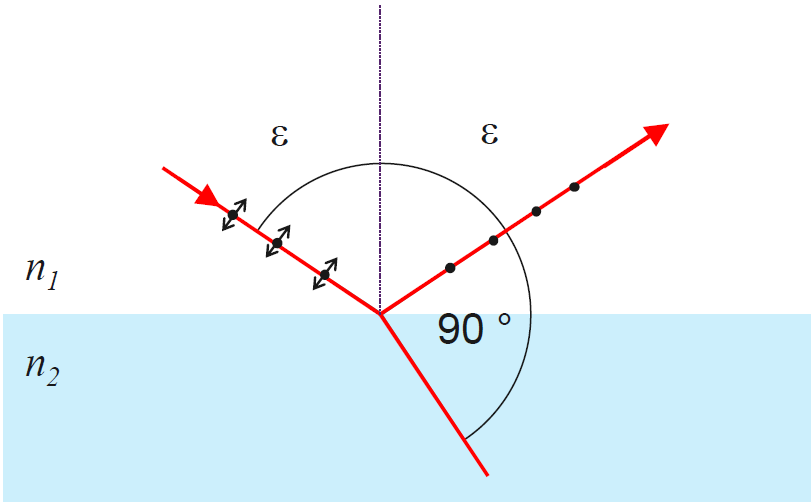
\includegraphics[width=\columnwidth]{images/brewster_winkel.png}
\end{minipage}
\hfill
\begin{minipage}{0.6\columnwidth}
    Unter dem \textbf{Brewster Winkel} wird nur \textbf{linear polarisiertes Licht} zurückgeworfen. 

    Der ins Medium 2 eindringende Strahl steht dabei \textbf{senkrecht} auf dem reflektierten Strahl
    $$ \boxed{  \tan(\varepsilon) = \frac{n_2}{n_1}  }$$
\end{minipage}


\subsubsection{Zirkulare Polarisation}

\begin{outline}
    \1 $x$ und $y$ Komponenten haben die \textbf{gleiche Amplitude}
    \1 \textbf{Phasendifferenz von 90°} 
\end{outline}

\smallskip

\begin{minipage}{0.38\columnwidth}
    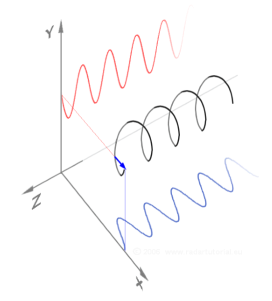
\includegraphics[width=\columnwidth]{images/Zirkulare_Polarisation.png}
\end{minipage}
\hfill
\begin{minipage}{0.58\columnwidth}
    Positive zirkulare Polarisation $\sigma ^+$ \\
    Positive zirkulare Polarisation $\sigma ^-$ 

    $$ \boxed{ \vec{E} = \begin{pmatrix} E_0 \cos(2 \pi ft-kz) \\ E_0 \sin(2 \pi ft -kz) \\ 0 \end{pmatrix}  } $$

    \begin{center}
        $\vec{E}$ kann nicht zu $\vec{0}$ werden 
    \end{center}  
\end{minipage}


\subsubsection{Elliptische Polarisation}

\vspace{-0.2cm}

\begin{minipage}[c]{0.58\columnwidth}
    \begin{outline}
        \1 $x$ und $y$ Komponenten haben \textbf{unterschiedliche Amplituden}
        \1 \textbf{beliebige Phasendifferenz}
    \end{outline}
\end{minipage}
\hfill
\begin{minipage}[c]{0.4\columnwidth}
    $$ \boxed{  \vec{E} = 
    \begin{pmatrix} 
        E_0 \cos(2 \pi ft-kz) \\ 
        E_0 \cos(2 \pi ft -kz + \varphi) \\ 
        0 
    \end{pmatrix}  } $$
\end{minipage}


\subsubsection{Doppelbrechung}

Doppelbrechung ist eine anisotropische Eigenschaft von Kristrallen \\
Diese Kristalle haben unterschiedliche Brechungsindizes in unterschiedliche Richtungen 

\smallskip

Nach einer gewissen Zeit $t$ haben die $x$- und $y$-Komponente einen Phasenunterschied. \\
\textrightarrow\  $x$ und $y$ bewegen sich unterschiedlich schnell fort 

\begin{center}
    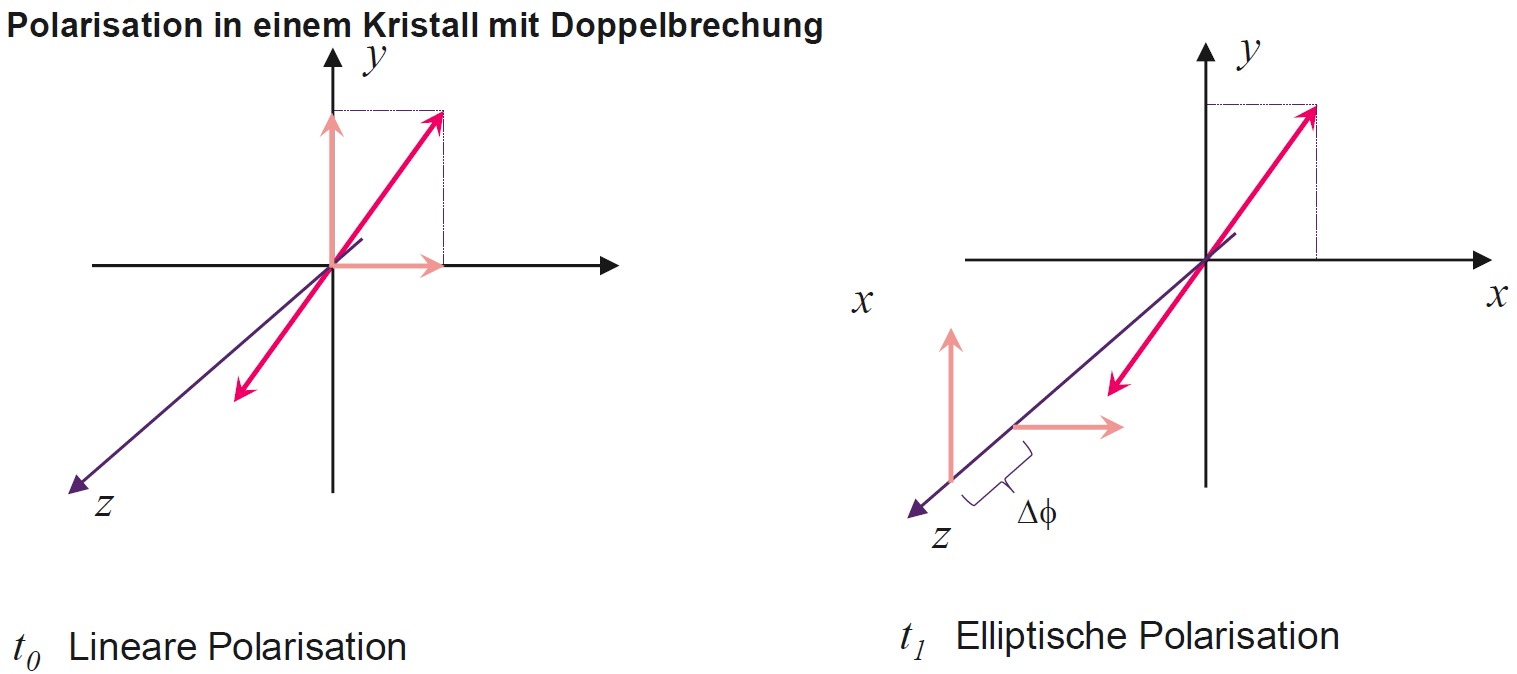
\includegraphics[width=0.8\columnwidth]{images/kristall_mit_doppelbrechung.png}
\end{center}

\vspace{-0.2cm}


\subsection{Streuung}

\subsubsection{Diffuse Streuung}

Streuung des Lichts an Teilchen von Dimensionen $d \gg \lambda$ 

\begin{minipage}{0.45\columnwidth}
    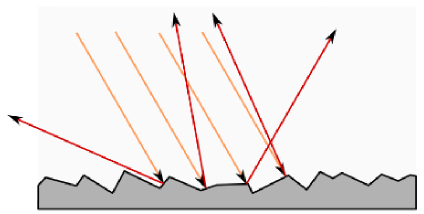
\includegraphics[width=\columnwidth]{images/diffuse_streuung.jpg}
\end{minipage}
\hfill
\begin{minipage}{0.53\columnwidth}
    \begin{itemize}
        \item Licht als \textbf{Strahlen}
        \item Reflexion in alle Richtungen
        \item Keine bevorzugte Richtung \\
            unabhängig von $\lambda$ 
        \item Wolken, Nebel 
        \item milchiche Lösungen 	  
    \end{itemize}
\end{minipage}


\subsubsection{Rayleigh-Streuung}

Streuung des Lichts an Teilchen von Dimensionen $d < \lambda$ (atomare Grösse)

\smallskip

\begin{minipage}{0.34\columnwidth}
    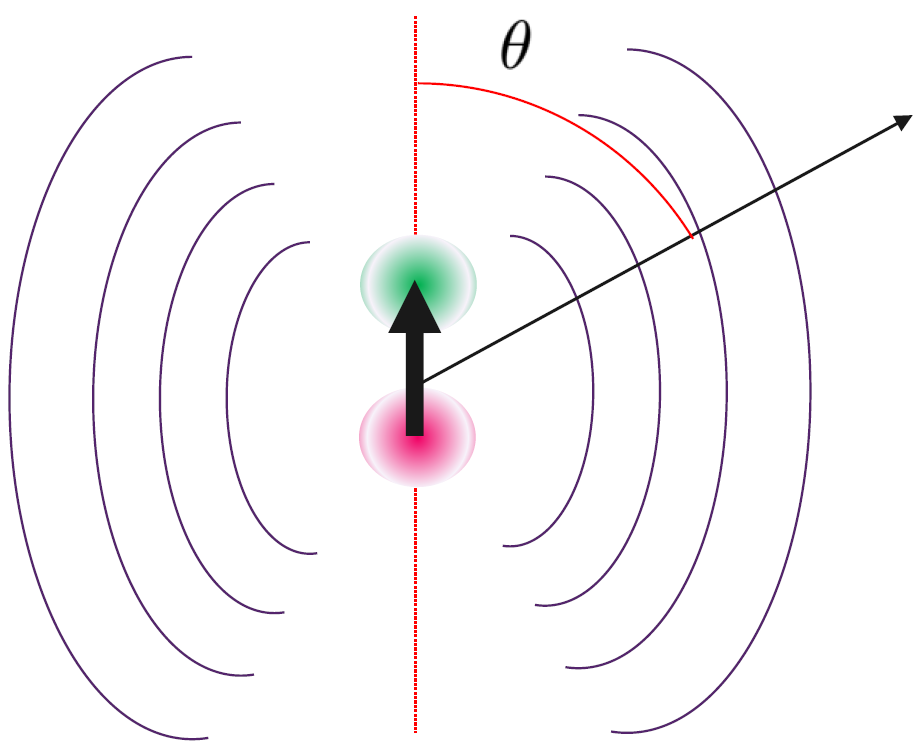
\includegraphics[width=\columnwidth]{images/rayleigh_streuung.png}
\end{minipage}
\hfill
\begin{minipage}{0.64\columnwidth}
    $$ \boxed{ I(\theta) = A \, f^4 \, \frac{\sin^2 (\theta)}{r^2} } $$

    \textrightarrow\  hochfrequentes Licht wird viel stärker abgestrahlt!

    \begin{itemize}
        \item Licht als \textbf{Wellen} senkrecht zur Ausbreitungsrichtung 
        \item Abstrahlmuster eines Dipols
        \item Himmel tagsüber blau 
        \item Himmel abends rötlich	  
    \end{itemize}
\end{minipage}


        \section{Optische Apparaturen}

\subsection{Abbildungssysteme -- Auge}

\subsubsection{Terminologie des Auges}

\paragraph{Sehwinkel $\varepsilon$}

\begin{minipage}{0.48\columnwidth}
    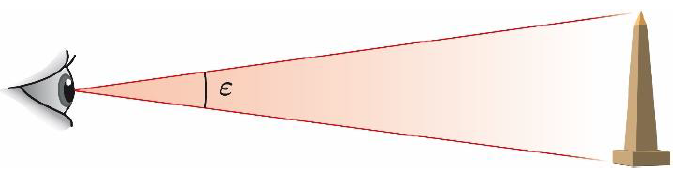
\includegraphics[width=0.9\columnwidth]{images/sehwinkel.png}
\end{minipage}
\hfill
\begin{minipage}{0.48\columnwidth}
    Die Grösse, in der ein Gegenstand dem betrachtenden Auge erscheint \textbf{(in Bogenminuten)} $\cbl{1 \degree \Leftrightarrow\ 60'}$
\end{minipage}


\medskip

\para{Auflösung}

Minimaler Winkelabstand $\varepsilon _{\rm min}$, den zwei Punkte haben müssen, damit sie noch getrennt wahrgenommen werden. \\
Normalsichtiges Auge: Auflösung ca. 1 Bogenminute ($1'$)

\medskip


\para{Sehschärfe}

Reziprokwert der Auflösung

$$ \boxed{ S = \frac{1}{\varepsilon _{\rm min}} \qquad \text{beim Menschen also } S = 1  } $$ 


\medskip

\paragraph{Deutliche Sehweite $\bm{s}$ (normierte Betrachtungsdistanz)}

Damit die Vergrösserungen von Lupen und Mikroskopen eindeutig bestimmt werden können, wird eine \textbf{deutliche Sehweite} definiert:

$$ \boxed{ s = 25 \, \mathrm{cm} = 0.25 \, \mathrm{m}  } $$ 


\subsubsection{Kurzsichtigkeit vs. Weitsichtigkeit}

\begin{minipage}{0.48\columnwidth}
    \raggedright
    \textbf{Kurzsichtigkeit} 

    \begin{itemize}
        \item Augapfel zu lang
        \item Konkave Streulinse als\\
            Korrektur
        \item Brille rückt Gegenstand näher heran 
    \end{itemize}
\end{minipage}
\hfill
\begin{minipage}{0.48\columnwidth}
    \raggedright
    \textbf{Weitsichtigkeit}

    \begin{itemize}
        \item Augapfel zu kurz
        \item Konvexe Sammellinse als Korrektur
        \item Brille rückt Gegenstand weiter weg 
    \end{itemize}
\end{minipage}


\subsection{Abbildungssysteme -- Fotoapparat}


\begin{minipage}{0.66\columnwidth}
    \paragraph{Bildgrösse $\bm{B}$} 

    Die Bildweite $b$ ist normalerweise viel kleiner als die
    Gegenstandsweite $g$ und daraus folgt:
\end{minipage}
\hfill
\begin{minipage}{0.3\columnwidth}
    $$ \boxed{ B = \frac{f}{g} \, G }$$
\end{minipage}

\smallskip


\begin{minipage}{0.66\columnwidth}
    \paragraph{Lichtstärke $\bm{H}$} 

    Die Intensität des Lichts auf dem Film ist gegeben durch
\end{minipage}
\hfill
\begin{minipage}{0.3\columnwidth}
    $$ \boxed{ H = \left(  \frac{d}{f} \right)^2 = q^2 } $$
\end{minipage}

\smallskip


\begin{minipage}{0.66\columnwidth}
    \paragraph{Blendenzahl $\bm{Z}$} 
    z.B.: 1, 1.4, 2, 2.8, 4, 5.6, \ldots
\end{minipage}
\hfill
\begin{minipage}{0.3\columnwidth}
    $$ \boxed{ Z = \frac{1}{q} = \frac{1}{\sqrt{H}}  } $$
\end{minipage}


\smallskip

\paragraph{Belichtung $\bm{E}$, Belichtungszeit $\bm{t}$} 

\begin{minipage}{0.66\columnwidth}
    $$ \boxed{ E = H t \approx q^2 t} $$
\end{minipage}
\hfill
\begin{minipage}{0.3\columnwidth}
    $$ \boxed{ t = \frac{G}{v} = \frac{g}{f} \frac{B}{v} } $$
\end{minipage}




\smallskip

\paragraph{Schärfentiefe} 

In der Filmebene ergibt sich vom Punkt $G$ kein scharfer Bildpunkt, sondern ein \textbf{Unschärfekreis} mit dem Durchmesser $u$. 

Es wird folgende Gegenstandsweite $g$ in den Unschärfekreis abgebildet:

\begin{minipage}{0.65\columnwidth}
    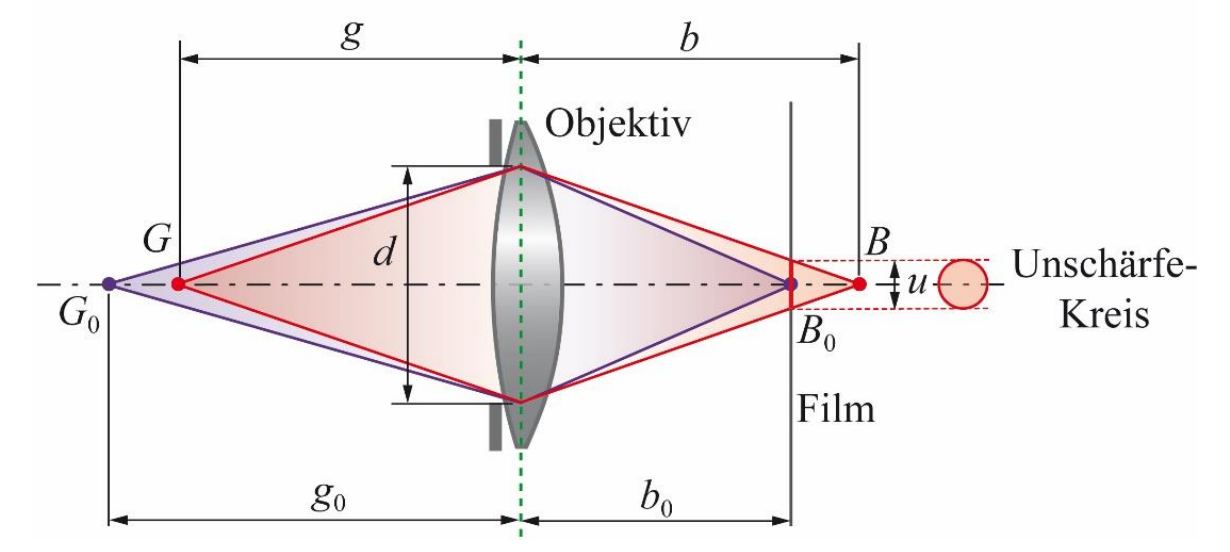
\includegraphics[width=\columnwidth]{images/schaerfentiefe.png}
\end{minipage}
\hfill
\begin{minipage}{0.3\columnwidth}
    $$\boxed{ \frac{1}{g} = \frac{1}{g_0} \pm \frac{u}{q \, f^2}  } $$
\end{minipage}

\begin{ctabular}{c l c}
	$b$     & Bildweite                                             & $[b] = \meter$    \\
	$b_0$   & $\text{Bilddlistanz}_0$                               & $[b_0] = \meter$  \\
	$B$     & $\text{Bildgrösse}$                                   & $[B] = \meter$    \\
	$B_0$   & $\text{Bild}_0$                                       & $[B_0] = \meter$  \\
	$g$     & Gegenstandsweite ($G$ zu Objektiv)                    & $[g] = \meter$    \\
	$g_0$   & $\text{Gegenstandsdistanz}_0$ ($G_0$ zu Objektiv)     & $[g_0] = \meter$  \\
	$G$     & Gegenstandsgrösse                                     & $[G] = \meter$    \\
	$G_0$   & $\text{Gegenstandsgrösse}_0$                          & $[G_0] = \meter$  \\
	$f$     & Brennweite                                            & $[f] = \meter$    \\
	$u$     & Durchmesser Unschärfekreis                            & $[u] = \meter$    \\
	$d$     & Durchmesser Blendenöffnung                            & $[d] = \meter$
\end{ctabular}


\subsection{Abbildungssysteme -- Lupe}

\begin{minipage}{0.48\columnwidth}
    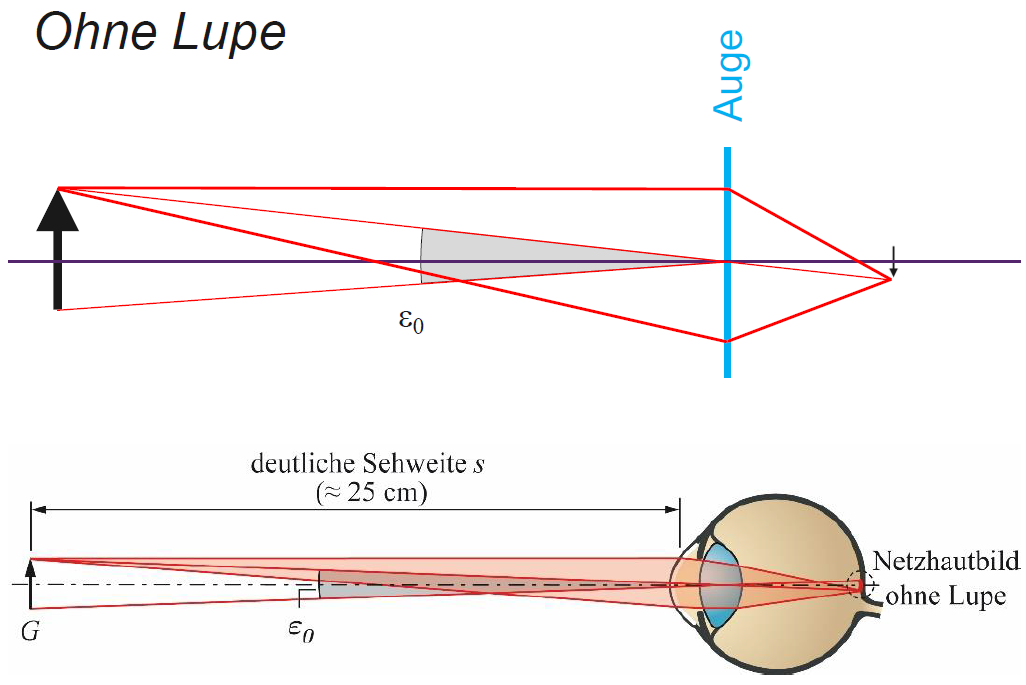
\includegraphics[width=0.9\columnwidth]{images/ohne_lupe.png}

    $$ \boxed{ \tan(\varepsilon_0) = \frac{G}{s} } $$
\end{minipage}
\hfill
\begin{minipage}{0.48\columnwidth}
    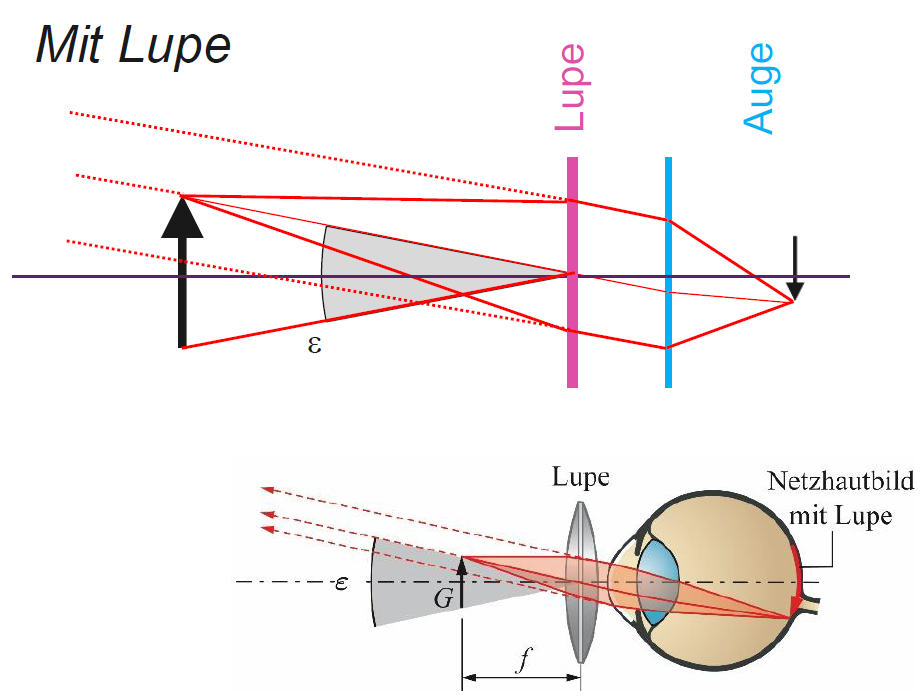
\includegraphics[width=0.9\columnwidth]{images/mit_lupe.png}

    $$ \boxed{ \tan(\varepsilon) = \frac{G}{f} } $$
\end{minipage}

$$ \boxed{ V = \frac{\tan(\varepsilon)}{\tan(\varepsilon_0)} = \frac{s}{f} } $$

\begin{ctabular}{c l c}
	$\varepsilon_i$ & Sehwinkel                                 & $[\varepsilon_i] = \degree$   \\
	$s$             & Deutliche Sehweite $s =0.25 \, \meter$    & $[s] = \meter$                \\
	$f$             & Brennweite                                & $[f] = \meter$                \\
	$V$             & Vergrösserung                             & $[V] = 1$                     \\
    $G$             & Gegenstandsgrösse                         & $[G] = \meter$                
\end{ctabular}


\subsection{Abbildungssysteme -- Fernrohr}

Es wird zuerst ein vergrössertes Bild erzeugt, welchs selber wiederum mit einer Lupe betrachtet wird.

\begin{center}
    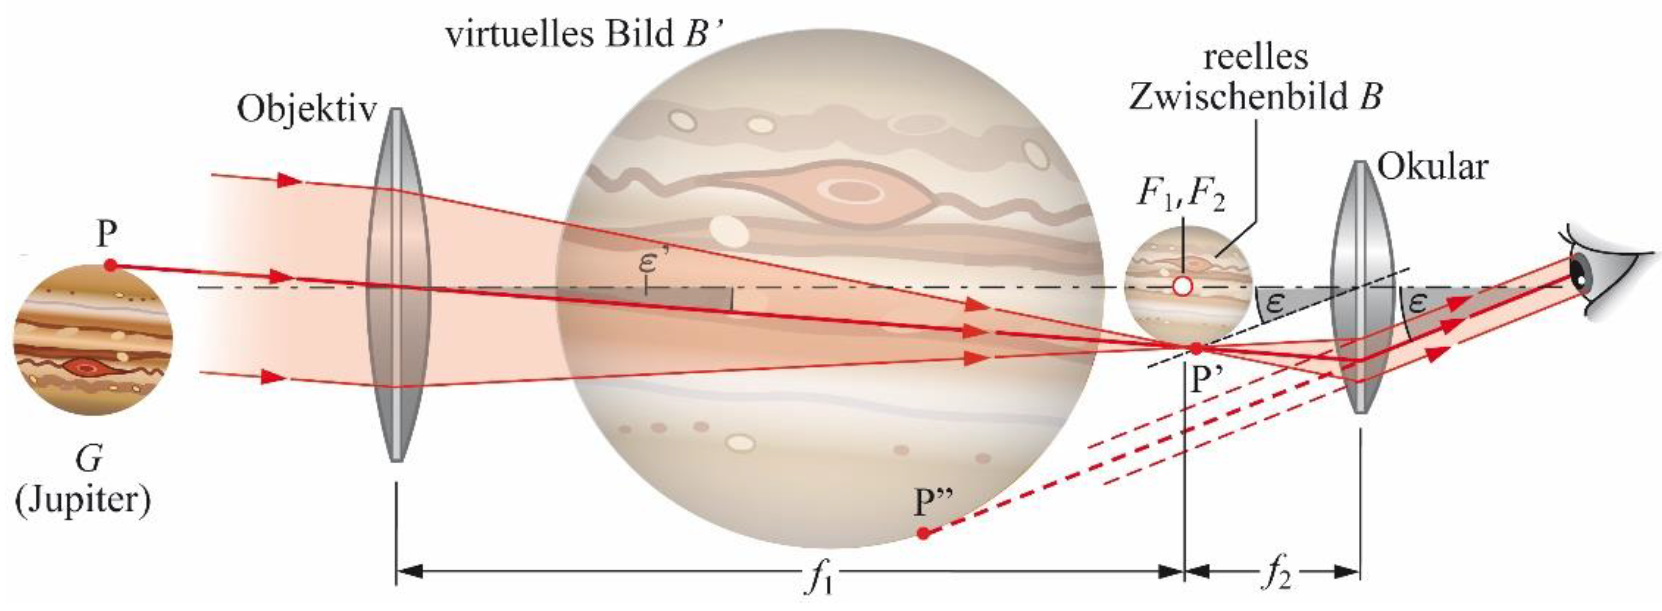
\includegraphics[width=0.9\columnwidth]{images/fernrohr.png}
\end{center}

\begin{minipage}[c]{0.48\columnwidth}
    $$ \boxed{ V = \frac{\tan(\varepsilon)}{\tan(\varepsilon_0)} = \frac{\frac{B}{f_2}}{\frac{B}{f_1} } = \frac{f_1}{f_2} } $$
\end{minipage}
\hfill
\begin{minipage}[c]{0.48\columnwidth}
    \begin{ctabular}{c l c}
        $\varepsilon_i$     & Sehwinkel                                     & $[\varepsilon_i] = \degree$   \\
        $f_i$               & Brennweite                                    & $[f_i] = \meter$              \\
        $V$                 & Vergrösserung                                 & $[V] = 1$                     \\
        $B$                 & Bildgrösse                                    & $[B] = \meter$                
    \end{ctabular}
\end{minipage}

\columnbreak


\subsection{Abbildungssysteme -- Mikroskop}

Es wird zuerst ein vergrössertes Bild erzeugt, welchs selber wiederum mit einer Lupe betrachtet wird. 

\medskip
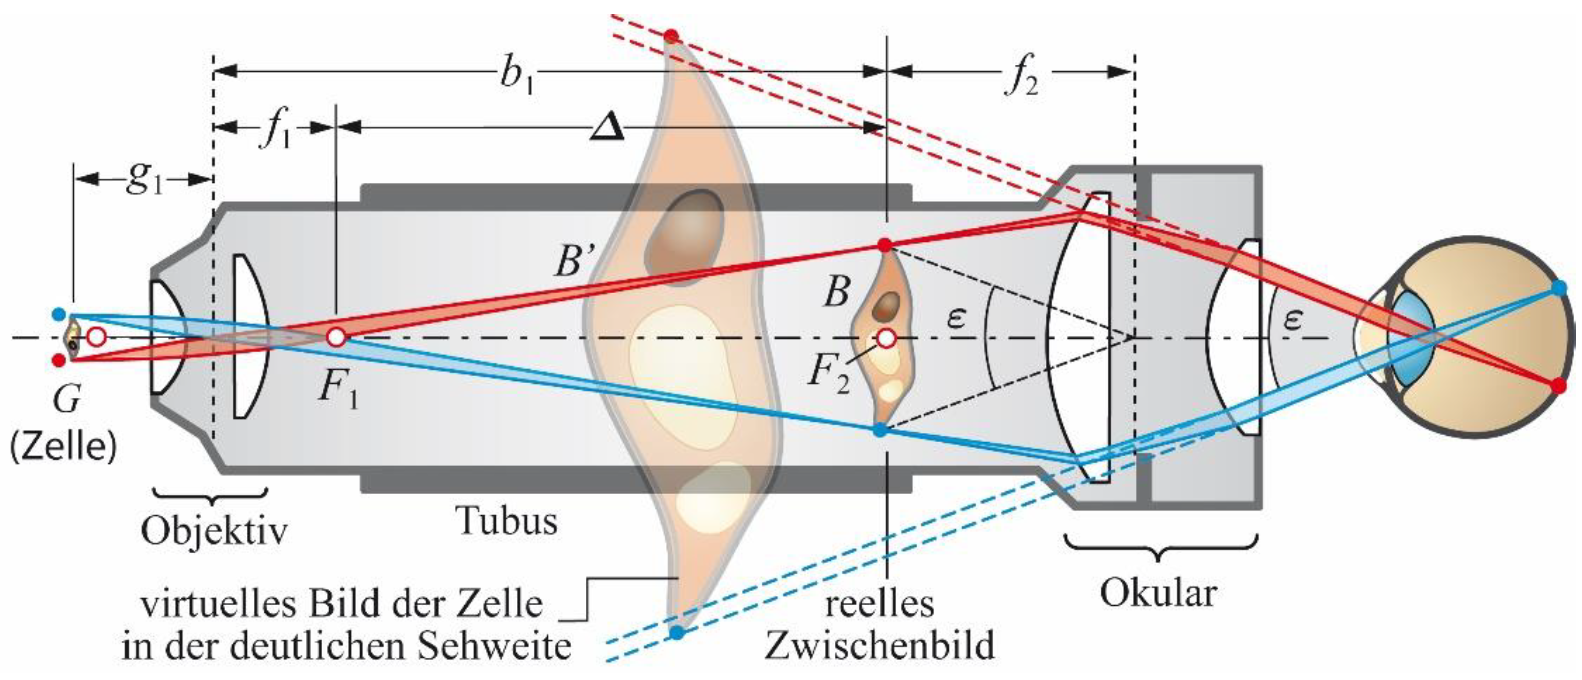
\includegraphics[width=0.9\columnwidth]{images/mikroskop.png}

$$ \boxed{ V = \underbrace{ \frac{\Delta}{f_1} }_{V_1} \cdot \underbrace{ \frac{s}{f_2} }_{V_2} = \frac{\tan(\varepsilon)}{\tan(\varepsilon_0)} = \frac{\frac{B}{f_2}}{\frac{G}{s}} = \frac{B}{G} \frac{s}{f_2} = \frac{b_1}{g_1} \frac{s}{f_2} } $$

\begin{ctabular}{c l c}
	$\varepsilon_i$     & Sehwinkel                                     & $[\varepsilon_i] = \degree$   \\
	$s$                 & Deutliche Sehweite $s =0.25 \, \meter$        & $[s] = \meter$                \\
	$f_i$               & Brennweite                                    & $[f_i] = \meter$              \\
	$V$                 & Vergrösserung                                 & $[V] = 1$                     \\
	$\Delta$            & optische Tubuslänge (Abstand der Brennpunkte) & $[\Delta] = \meter$           \\
	$b_1$               & Bildweite                                     & $[b_1] = \meter$              \\
	$g_1$               & Gegenstandsweite                              & $[g_1] = \meter$              \\
	$B$                 & Bildgrösse                                    & $[B] = \meter$                \\
	$G$                 & Gegenstandsgrösse                             & $[G] = \meter$
\end{ctabular}


\subsection{Farbentheorie}

\begin{description}
    \item[Spektralfarben:] Die gesamten Lichtfarben
    \item[Monochromatisches Licht:] Nur eine einzige Wellenlänge (Farbe) 
\end{description}


\subsubsection{Farbmischungen}

\begin{minipage}{0.42\columnwidth}
    \textbf{Additive Farbmischung}

    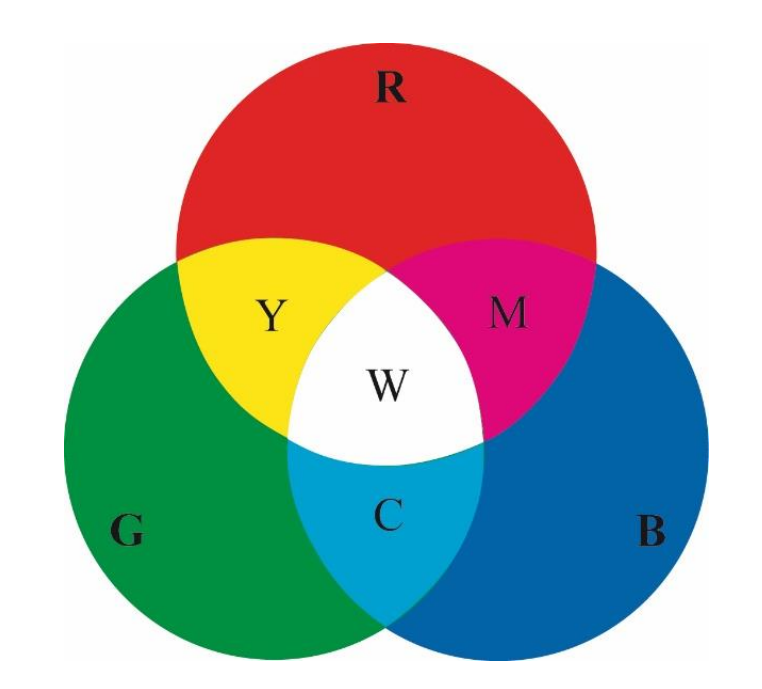
\includegraphics[width=\columnwidth]{images/additiveFarbmischung.png}
\end{minipage}
\hfill
\begin{minipage}{0.42\columnwidth}
    \textbf{Subtraktive Farbmischung}

    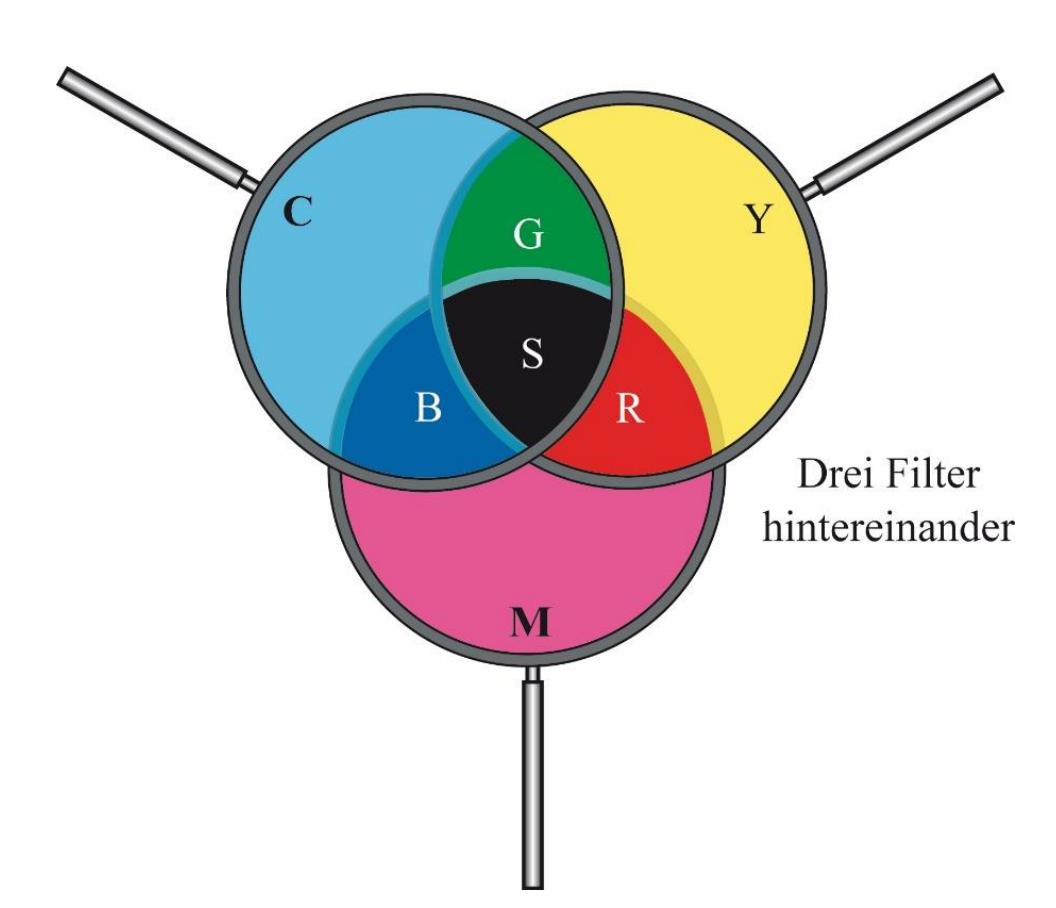
\includegraphics[width=\columnwidth]{images/SubtraktiveFarbmischung.png}
\end{minipage}


    
        \columnbreak

        \part{Schwingungen}
		\section{Ungedämpfte Schwingungen}

\subsection{Schwingungen -- Übersicht}

\paragraph{Freie Schwingung}

Wird ein schwingungsfähiges System aus dem Gleichgewichtszustand gebracht 
und dann sich selbst überlassen, so führt es freie Schwingungen oder Eigenschwingungen aus.


\medskip

\paragraph{Erzwungene / Fremderregte Schwingung}

Wird ein System von aussen durch periodische oder auch nichtperiodische Störungen zum
Schwingen veranlasst, wird von fremderregten Schwingungen gesprochen. 


\medskip

\paragraph{Selbsterregte Schwingung}

Ein schwingungsfähiges System kann unter Umständen einer Energiequelle Energie entziehen
und diese der eigenen Schwingung selbst zuführen, so dass die Schwingung trotz einer
eventuell vorhandenen Dämpfung nicht abklingt. 


\subsection{Freie Schwingungen}

\subsubsection{Terminologie}

\vspace{-0.2cm}
$$ \boxed{  y(t) = A \cdot \sin(\omega \, t + \varphi) } $$
\[
    \dot{y}(t) =  v(t) = A \cdot \omega \cdot \cos(\omega \, t + \varphi) 
    \qquad \qquad \quad
    \ddot{y}(t) = a(t) = - A \cdot \omega^2 \cdot \sin(\omega \, t + \varphi) 
\]
\[
    \boxed{ f = \frac{\omega}{2 \, \pi} }
    \qquad \qquad \qquad \qquad \qquad \qquad
    \boxed{ T = \frac{1}{f} = \frac{2 \, \pi}{\omega} }
\]


\renewcommand{\arraystretch}{1.3}
\begin{ctabular}{clc}
    $y(t)$          & Position zum Zeitpunkt $t$        & $[y(t)] = \meter$                             \\
    $\dot{y}(t)$    & Geschwindigkeit zum Zeitpunkt $t$ & $[\dot{y}(t)] = \frac{\meter}{\second}$       \\ 
    $\ddot{y}(t)$   & Beschleunigung  zum Zeitpunkt $t$ & $[\ddot{y}(t)] = \frac{\meter}{\second^2}$    \\ 
    $A$             & Amplitude                         & $[A] = \meter$                                \\
    $\omega$        & Winkelgeschwindingkeit            & $[\omega] = \frac{\rad}{\second}$             \\
    $\varphi$       & Phase                             & $[\varphi] = \rad$                            \\ 
    $T$             & Periodendauer                     & $[T] = \second$                               \\
    $f$             & Frequenz                          & $[f] = \frac{1}{\second}$
\end{ctabular}
\renewcommand{\arraystretch}{1}


\example{Federpendel}

\begin{minipage}{0.48\columnwidth}
    $$F_{\rm res} = m \cdot a = m \cdot \ddot{x}$$ 
\end{minipage}
\hfill
\begin{minipage}{0.48\columnwidth}
    $$F_{\rm Feder} = -k \cdot x$$
\end{minipage}

$$ \text{Kräftegleichgewicht:} \quad m \cdot \ddot{x} = -k \cdot x $$
\[ 
    \boxed{ \text{DGL: } \ddot{x} = - \omega^2 \cdot x \quad \text{mit } \omega^2 = \frac{k}{m} } 
    \qquad \quad
    \text{Allgemeine Lösung:} \quad  x(t) = A \cdot \sin(\omega \, t + \varphi) 
\]

\begin{ctabular}{clc}
    $m$     & Masse             & $[m] = \meter$                    \\
    $k=c$   & Federkonstante    & $[k] = \frac{\newton}{\meter}$
\end{ctabular}


\subsubsection{Harmonische Schwingung -- Energiebetrachtung}

\vspace{-0.2cm}

\[
    \cbl{x(t) = A \cdot \sin(\omega \, t + \varphi)} 
    \qquad \qquad \qquad
    \cvt{\dot{x}(t) = \omega \cdot A \cdot \cos(\omega \, t + \varphi)}
\]

\vspace{-0.2cm}

\begin{align*}
    E_{\rm tot} &= E_{\rm pot} + E_{\rm kin} = \frac{k \cdot \cbl{x^2} }{2} + \frac{m \cdot \cvt{\dot{x}^2 } }{2}   \\
                &= \frac{k}{2} A^2 \cdot \sin^2(\omega \, t + \varphi) + \frac{m}{2} \omega^2  A^2 \cdot \cos^2(\omega \, t + \varphi) \\
                &= \frac{k A^2}{2} ( \sin^2(\omega \, t + \varphi) + \cos^2(\omega \, t + \varphi) )
\end{align*}

$$ \boxed{ E_{\rm tot} = \frac{k \cdot A^2}{2} } $$


\subsection{Beschreibung einer 1D-Schwingung}

\subsubsection{Zeitbreich}

\begin{minipage}[t]{0.42\columnwidth}
    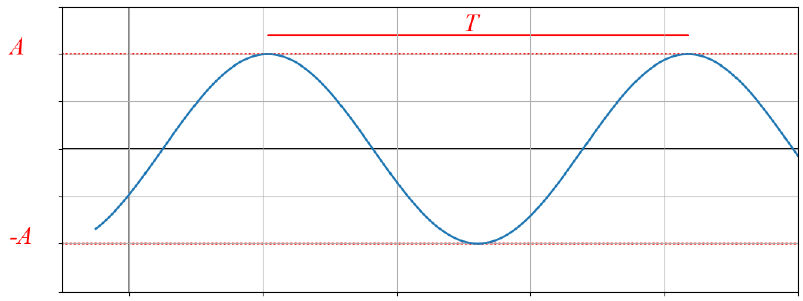
\includegraphics[width=\columnwidth, align=t]{images/zeitbereich.png}
\end{minipage}
\hfill
\begin{minipage}[t]{0.52\columnwidth}
    Auslenkung in Abhängigkeit der Zeit \\
    Beispiel: Oszilloskop 
    $$ x(t) = A \cdot \sin(\omega \, t + \varphi) $$
\end{minipage}


\subsubsection{Zeigerdarstellung}

\begin{minipage}[c]{0.4\columnwidth}
    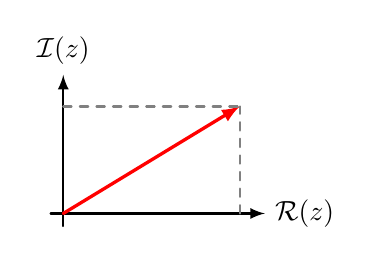
\begin{tikzpicture}
    [>=latex, 
    line cap=round,
    line join=round,
    scale=0.8]

    \draw[->, thick] (-0.2, 0  ) -- (3.2, 0 ) node[right] {$\mathcal{R}(z)$};
    \draw[->, thick] (0,   -0.2) -- (0,  2.2) node[above] {$\mathcal{I}(z)$};
        
    \draw[->, very thick, red] (0, 0) -- (2.8, 1.7);

    % Hilfslinien
    \draw[dashed, thick, gray] (2.8, 0) -- (2.8, 1.7);
    \draw[dashed, thick, gray] (0, 1.7) -- (2.8, 1.7);
\end{tikzpicture}
\end{minipage}
\hfill
\begin{minipage}[c]{0.56\columnwidth}
    Auslenkung als Zeiger (komplexe Zahl), der um den Ursprung rotiert 
    $$ z(t) = \underbrace{ x(t) }_{\substack{\mathcal{R}(z)}} + i \, \underbrace{ y(t) }_{\substack{ \mathcal{I}(z)}} $$
\end{minipage}


\subsubsection{Phasenraum}

\begin{minipage}[c]{0.4\columnwidth}
    
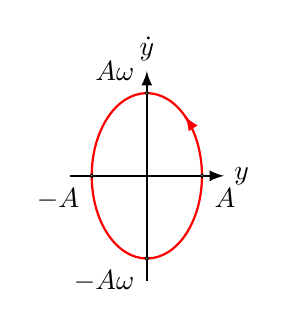
\begin{tikzpicture}[>=latex, scale=0.7]

  % Ellipse
  \draw[thick, red] (0,0) ellipse (1 and 1.5);

  % Achsen
  \draw[->, thick] (-1.4,0) -- (1.4,0) node[right] {$y$};
  \draw[->, thick] (0,-1.9) -- (0,1.9) node[above] {$\dot{y}$};

  % Beschriftungen
  \node at (1,0) [below right=1pt] {$A$};
  \node at (-1,0) [below left=1pt] {$-A$};
  \node at (0,1.5) [above left=1pt] {$A\omega$};
  \node at (0,-1.5) [below left=1pt] {$-A\omega$};

  % Punkte auf Ellipse
  \filldraw[white, draw=black] (1,0) circle (0.03);
  \filldraw[white, draw=black] (-1,0) circle (0.03);
  \filldraw[white, draw=black] (0,1.5) circle (0.03);
  \filldraw[white, draw=black] (0,-1.5) circle (0.03);

  % Pfeil auf der Ellipse
  \draw[->, red, thick, domain=45:46] plot ({cos(\x)}, {1.5*sin(\x)});
\end{tikzpicture}
\end{minipage}
\hfill
\begin{minipage}[c]{0.54\columnwidth}
    Darstellung der Position $y$ und der Ableitung (Geschwindigkeit)
\end{minipage}


\subsection{Pendel}

\subsubsection{Fadenpendel}

\begin{minipage}{0.27\columnwidth}
    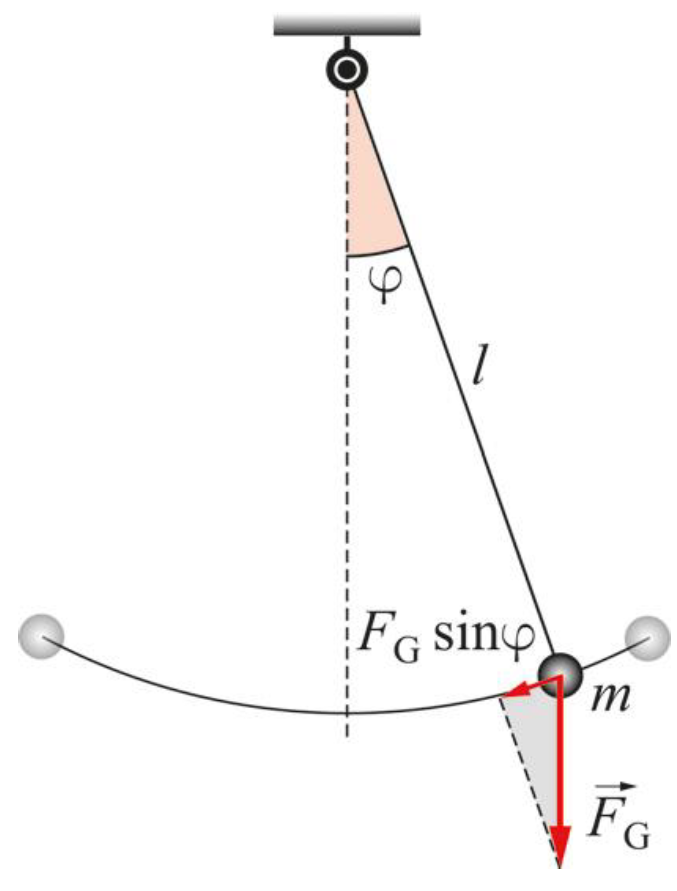
\includegraphics[width=\columnwidth]{images/fadenpendel.png}
\end{minipage}
\hfill
\begin{minipage}{0.7\columnwidth}
    $$ F_R = F_G \cdot \sin(\varphi) = m \cdot g \cdot \sin(\varphi) \approx m \cdot g \cdot \varphi $$
    $$ x = \varphi \cdot l \quad \rightarrow \quad \varphi = \frac{x}{l} $$
    $$ \Rightarrow F_G = m \cdot g \cdot \frac{x}{l} $$
   
    $$ \text{Kräftegleichgewicht:} \quad  F = m \cdot \ddot{x} = - m \cdot g \, \frac{x}{l} $$
    $$ \boxed{ \text{DGL:} \quad  \ddot{x} = - \omega^2 \cdot x \quad \text{mit } \omega^2 = \frac{g}{l} } $$
\end{minipage}


\subsubsection{Drehpendel}

\begin{minipage}[t]{0.36\columnwidth}
    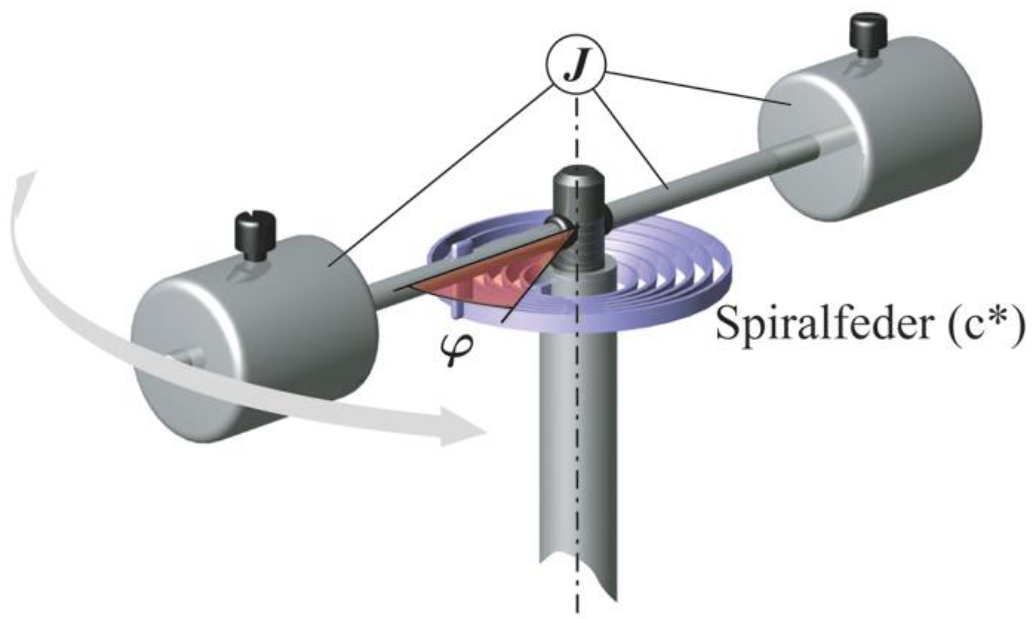
\includegraphics[width=\columnwidth, align=t]{images/drehpendel.png}
\end{minipage}
\hfill
\begin{minipage}[t]{0.6\columnwidth}
    \paragraph{Analogie ohne Rotation}

    \begin{minipage}[c]{0.58\columnwidth}
        $F = - k \cdot x$ \\
        $ M = - c^* \, \varphi$ 
    \end{minipage}
    \hfill
    \begin{minipage}[c]{0.4\columnwidth}
         $F = m \cdot a = m \cdot \ddot{x}$ \\
         $M = J \cdot \ddot{\varphi} $ 
    \end{minipage}

    $$ \text{Gleichgewicht:} \quad  J \cdot \ddot{\varphi} = - c^* \, \varphi $$
    $$ \boxed{ \text{DGL: } \ddot{\varphi} = - \omega^2 \cdot\varphi \quad \text{mit } \omega^2 = \frac{c^*}{J} }$$
\end{minipage}

\medskip

$\varphi$ folgt der gleichen DGL wie $x$ im Fall des Federpendels und hat die Lösung:
$$ \varphi(t) = \varphi_0 \cdot \sin(\omega \, t + \delta) $$

\renewcommand{\arraystretch}{1.3}
\begin{ctabular}{clc}
    $J$     & Trägheitsmoment   & $[J] = \kilogram \cdot \meter\squared$    \\
    $c^*$   & Winkelrichtgrösse & $[c^*] = \mathrm{\frac{N \, m}{rad}}$
\end{ctabular}
\renewcommand{\arraystretch}{1}



\subsubsection{Torisonpendel}
\begin{minipage}[t]{0.12\columnwidth}
    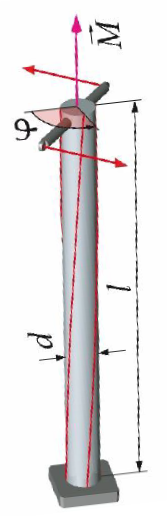
\includegraphics[width=\columnwidth, align=t]{images/torsionspendel.png}
\end{minipage}
\hfill
\begin{minipage}[t]{0.8\columnwidth}
    Variante des Drehpendels mit der Winkelrichtgrösse

    $$ \boxed{ c^* = \frac{\pi r^4 G}{2l} } $$  

    \begin{ctabular}{ll}
        $G$                 & Torsionsmodul \\
        $l$                 & Länge         \\
        $r = \frac{d}{2}$   & Radius
    \end{ctabular}
\end{minipage}


\subsubsection{Physikalisches Pendel}

\begin{minipage}{0.3\columnwidth}
    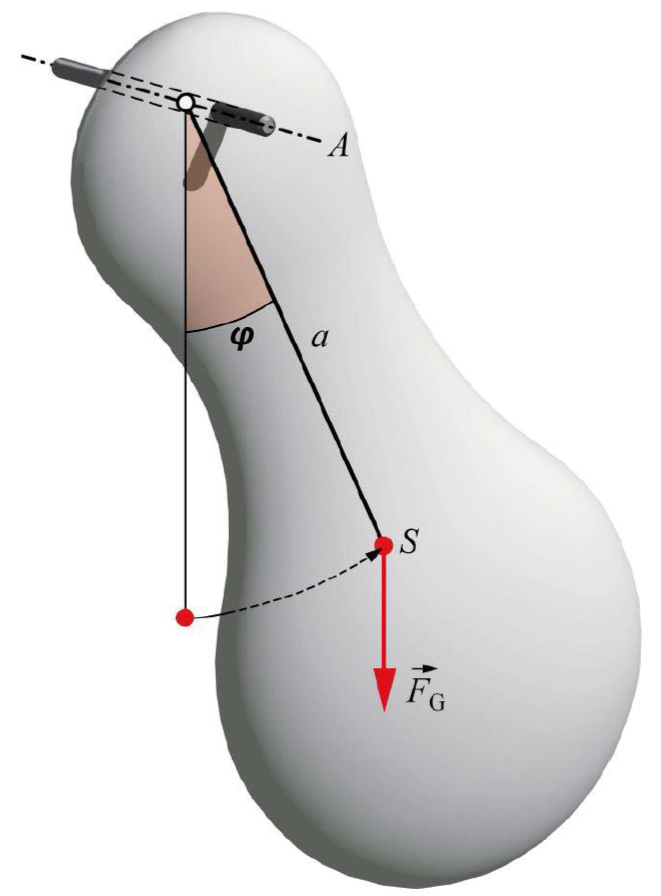
\includegraphics[width=\columnwidth]{images/physikalisches_pendel.png}
\end{minipage}
\hfill
\begin{minipage}{0.68\columnwidth}
    \vspace{-0.2cm}
    $$ M = - a \cdot \sin(\varphi) \cdot F_G = -a \cdot m \cdot g \cdot  \sin(\varphi) $$

    \begin{tabular}{ll}
        Bewegungsgleichung: & $M = J_A \cdot \ddot{\varphi}$                                            \\
        Gleichgewicht:      & $-a \cdot m \cdot g \cdot  \sin(\varphi) =  J_A \cdot \ddot{\varphi}$     \\
        Kleine Winkel:      & $-a \cdot m \cdot g \cdot \varphi =  J_A \cdot \ddot{\varphi}$            \\
    \end{tabular}

    $$ \boxed{ \text{DGL: } \ddot{\varphi} = -\omega^2 \, \varphi  \quad \text{mit } \omega^2 =  \frac{g}{L^*} = \frac{g \cdot a \cdot m}{J_A}  }$$
    $$ \boxed{L^* = \frac{J_A}{a \cdot m}} \qquad \boxed{J_A = J_s + m \cdot a^2 } $$  

    \medskip
    $\varphi$ folgt der gleichen DGL wie $x$ im Fall des Federpendels
\end{minipage}

\medskip

\paragraph{Physikalisches Pendel mit mehreren Massen}

\vspace{-0.2cm}

\begin{minipage}[c]{0.46\columnwidth}
    $$ \boxed{  T = \frac{2 \, \pi}{\omega} = 2 \, \pi \sqrt{\frac{J_{A1} + J_{A2}}{(a_1 \cdot m_1 + a_2 \cdot m_2) \cdot g}} } $$
\end{minipage}
\hfill
\begin{minipage}[c]{0.52\columnwidth}
    \textbf{ \textrightarrow\ $\bm{J}$-Tabelle im Anhang Abschnitt \ref{Massenträgheitsmomente}}
\end{minipage}

\begin{ctabular}{clc}
    $S$     & Schwerpunkt des Körpers           &                                           \\
    $J_s$   & Trägheitsmoment bzgl. $S$         & $[J_S] = \kilogram \cdot \meter\squared$  \\
    $a$     & Abstand Schwerpunkt -- Drehpunkt  & $[a] = \meter$                            \\
    $L^*$   & Reduzierte Länge                  & $[L^*] = \meter$                          \\
    $J_A$   & Trägheitsmoment um Aufhängepunkt  & $[J_A] = \kilogram \cdot \meter\squared$ 
\end{ctabular}


\subsection{Perkussionszentrum}

\textbf{Frage:} Wie weit vom Drehpunkt $A$ muss ein Impuls auf einen Körper ausgeübt werden, damit keine Kraft auf die Achse ausgeübt wird?

\smallskip

\textbf{Antwort:} Auf Höhe der \textbf{reduzierten Länge} $L^* = \frac{J_A}{a \cdot m}$

\begin{center}
    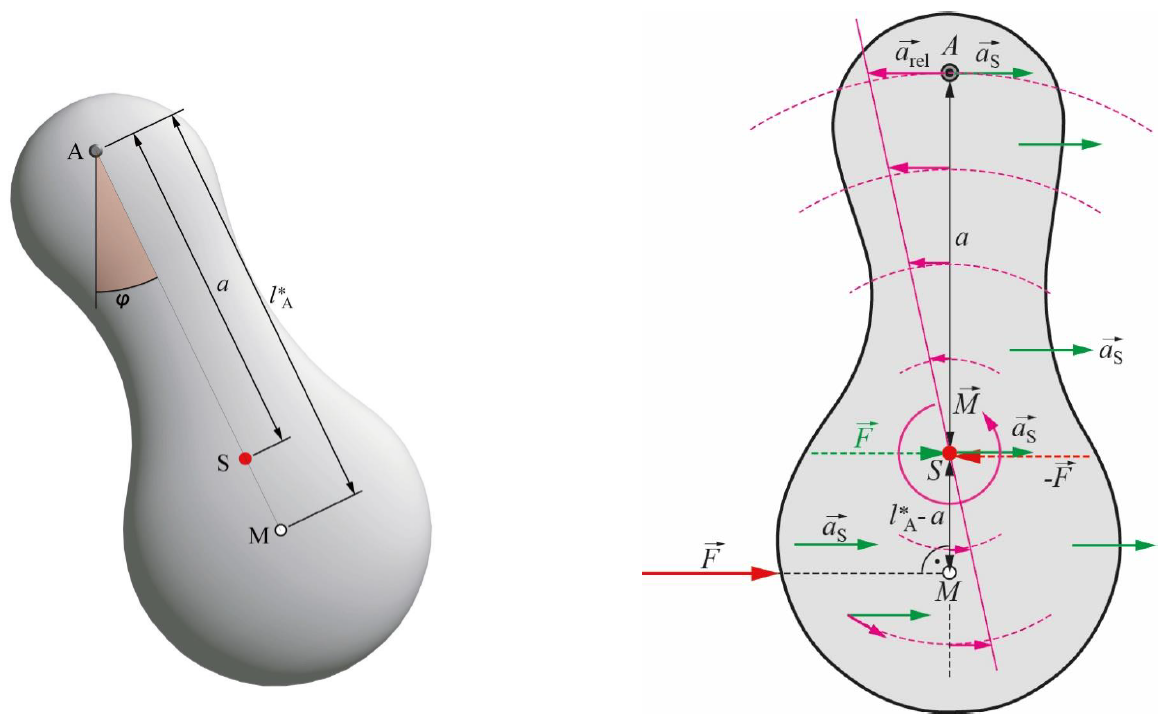
\includegraphics[width=0.7\columnwidth]{images/perkussionszentrum.png}
\end{center}



\subsection{Periodische Schwingung}

\begin{minipage}{0.4\columnwidth}
    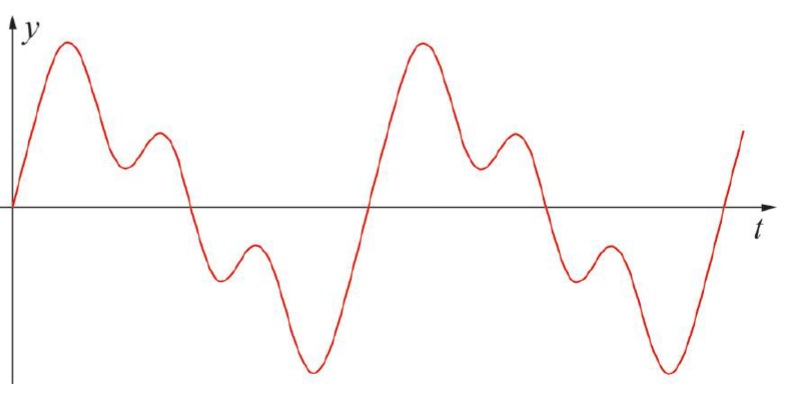
\includegraphics[width=\columnwidth]{images/periodische_schwingung.png}
\end{minipage}
\hfill
\begin{minipage}{0.56\columnwidth}
    Muster wiederholt sich mit Periode $T$
    $$ \boxed{ f(t) = f(t - T ) }$$
\end{minipage}

\smallskip

Periodische Schwingungen können im \textbf{Frequenzbereich} in eine \textbf{Grundschwingung} und \textbf{Oberschwingungen} \textbf{(Harmonische)} zerlegt werden. 

\begin{minipage}[c]{0.48\columnwidth}
    $$ \boxed{ f(t) = A_0 + \sum\limits_{n=1}^{\infty}  A_n \, \sin(n \cdot \omega + \varphi_n) } $$
\end{minipage}
\hfill
\begin{minipage}[c]{0.48\columnwidth}
    \renewcommand{\arraystretch}{1.3}
    \begin{tabular}{ll}
        $\omega_0 = \frac{2 \, \pi}{T}$     & Grundschwingung   \\
        $\omega_n = n \cdot \omega_0$       & $n$-te Harmonische
    \end{tabular}
    \renewcommand{\arraystretch}{1}
\end{minipage}





\subsubsection{Fourier-Analyse}

\vspace{-0.2cm}

$$ \boxed{ f(t) = A_0 +  \sum\limits_{n=1}^{\infty}  A_n \cdot \cos  \left(\frac{ 2 \, \pi \, n}{T} t \right) + \sum\limits_{n=1}^{\infty}  B_n \cdot \sin \left( \frac{ 2 \, \pi \, n}{T} t \right)  } $$


\begin{minipage}{0.48\columnwidth}
    \centering
    $ A_n = \frac{2}{T} \int\limits_{-T/2}^{T/2} f(t) \, \cos \Big(\frac{ 2 \, \pi \, n \, t}{T}  \Big)  \, \dd t $
\end{minipage}
\hfill
\begin{minipage}{0.48\columnwidth}
    \centering
    $A_0 = \frac{1}{T} \int\limits_{-T/2}^{T/2} f(t) \, \dd t $
\end{minipage}

\medskip

\begin{minipage}{0.48\columnwidth}
    \centering
    $ B_n = \frac{2}{T} \int\limits_{-T/2}^{T/2} f(t) \, \sin \Big(\frac{ 2 \, \pi \, n \, t}{T}  \Big)  \, \dd t $
\end{minipage}
\hfill\null%



\subsection{Signalmodulationen}

\begin{minipage}[t]{0.43\columnwidth}
    $$ \boxed{ x(t) = A \sin ( \omega t + \varphi)} $$ 

    \paragraph{ Amplitudenmodulation (AM)}
    Veränderung von $A$ 

    \medskip

    \paragraph{Frequenzmodulation (FM)}
    Veränderung von $\omega$
\end{minipage}
\hfill
\begin{minipage}[t]{0.55\columnwidth}
    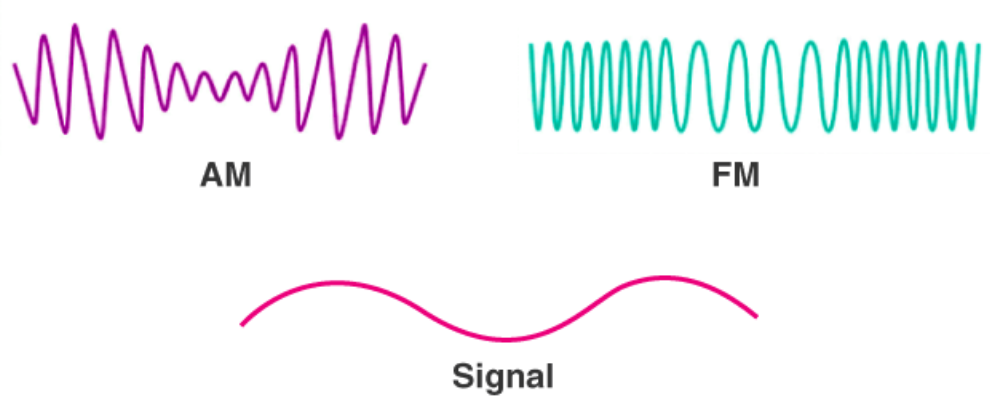
\includegraphics[width=\columnwidth, align=t]{images/AM_FM.png}
\end{minipage}



        
\section{Gedämpfte Schwingungen}

\subsubsection{Dämpfung mit konstanter Reibungskraft}

\vspace{-0.2cm}

$$ m \ddot{x}(t) = -k x(t) - \mu F_N \quad \text{für } \ddot{x}(t) > 0 $$
$$ m \ddot{x}(t) = -k x(t) + \mu F_N \quad \text{für } \ddot{x}(t) < 0 $$

\smallskip

\begin{minipage}[c]{0.7\columnwidth}
    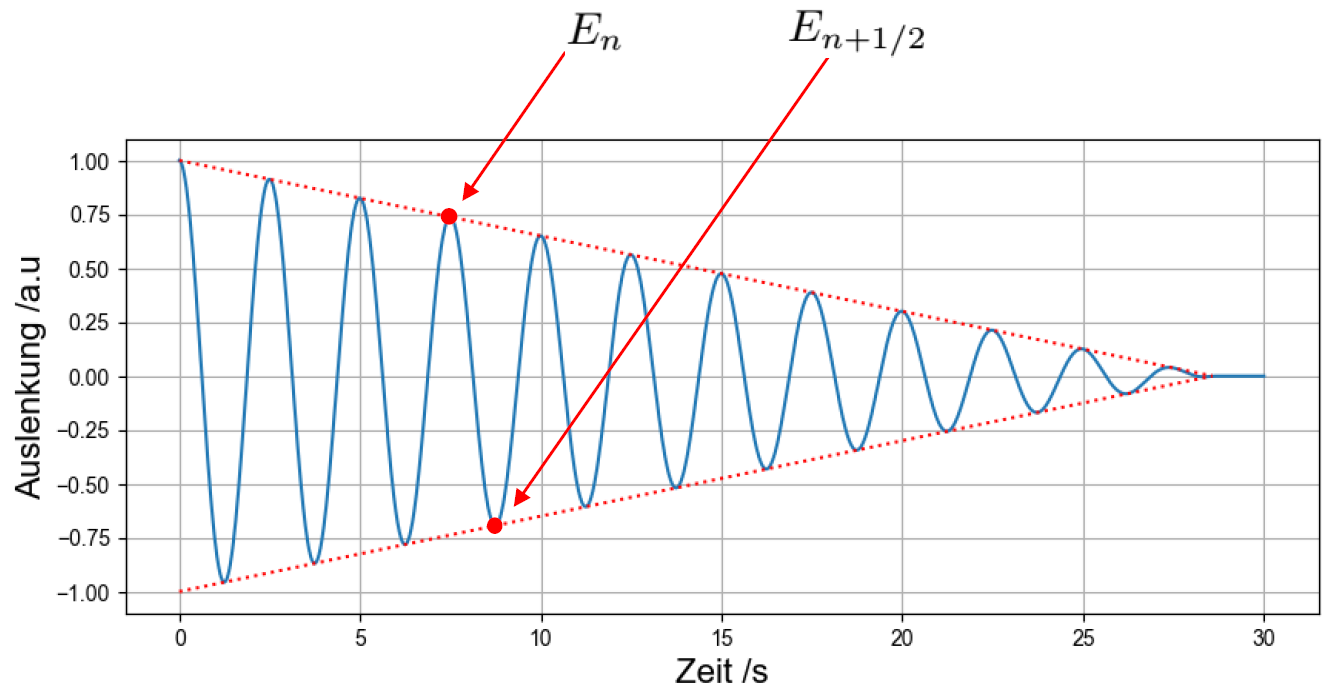
\includegraphics[width=\columnwidth]{images/gedaempfte_schwingungen_konst_reibung.png}
\end{minipage}
\hfill
\begin{minipage}[c]{0.28\columnwidth}
    $$ \boxed{ E = \frac{k \, A^2}{2} } $$
    $$ \boxed{ \Delta A = 4 \frac{F_R}{k}} $$
\end{minipage}


\begin{ctabular}{c l c}
    $E$         & Energie bei max. Auslenkung       & $[E] = \joule$                    \\
    $k=c$       & Federkonstante                    & $[k] = \frac{\newton}{\meter}$    \\
    $A$         & Amplitude bei max. Auslankung     & $[A] = \meter$                    \\
    $\Delta A$  & Amplitudenänderung pro Periode    & $[\Delta A] = \meter$             \\
    $F_R$       & Reibungskraft                     & $[F_R] = \newton$ 
\end{ctabular}


\subsection{Dämpfung proportional zur Geschwindigkeit}

\vspace{-0.2cm}
\[  
    \boxed{ \text{DGL:}  \quad \ddot{x}(t) + 2 \delta \, \dot{x}(t) + \omega^2 \, x(t) = 0 }
    \qquad \quad
    \boxed{ D = \frac{\delta}{\omega} = \frac{\kappa}{2 \omega} }
    \qquad \quad
    \boxed{ f = \frac{\Omega}{2 \, \pi} }
\]

\resizebox{\columnwidth}{!}{
    \begin{tabular}{lllll}
        \toprule
        Fall 1      & $\delta^2 - \omega^2 > 0$     & $D > 1$   & $x(t) = A e^{\lambda_1 t} + B e^{\lambda_2 t}$                            & Aperiodische Schwingung                                           \\
                    &                               &           &                                                                           & $\lambda_{1,2} = - \omega \left( D \pm \sqrt{D^2 -1} \right)$     \\
        \midrule    
        Fall 2      & $\delta^2 - \omega^2 < 0$     & $D < 1$   & $x(t) = A e^{- \delta t} \cdot \cos \left( \Omega t + \varphi \right)$    & Period. Schwingung (gedämpft)                                           \\
                    &                               &           &                                                                           & $\Omega^2 = \omega^2 \left( 1 - D^2 \right)$                      \\
        \midrule
        Fall 3      & $\delta^2 - \omega^2 = 0$     & $D = 1$   & $x(t) = (A + Bt) e^{- \delta t}$                                          & Grenzfall                                                         \\
        \bottomrule
    \end{tabular}
}

\medskip

\[
    \boxed{ \Omega^2 = \omega^2 - \delta^2  = \omega^2 - \left(\frac{\kappa}{2} \right)^2 }
    \qquad
    \boxed{ z \cdot \Lambda = \ln \left( \frac{A_n}{A_{n+z}} \right) = z \cdot \delta T = z \cdot \frac{\kappa}{2} T }
\]

\begin{ctabular}{c l c}
    $\delta = \frac{\kappa}{2}$ & Abklingkonstante                          & $[\kappa = \delta] = \frac{1}{\second}$ \\
    $\omega$                    & Kreisfrequenz ungedämpfte Schwingung      & $[\omega] = \frac{\rad}{\second}$ \\
    $D$                         & Dämpfungsgrad                             & $[D] = 1$ \\
    $\Omega$                    & Kreisfrequenz gedämpfte Schwingung        & $[\Omega] = \frac{\rad}{\second}$ \\
    $\Lambda$                   & Logarithmisches Dekrement                 & $[\Lambda] = 1$ \\
    $A_n$                       & Amplitude zum Zeitpunkt $t$               & $[A_n] = \meter$ \\
    $A_{n+z}$                   & Amplitude zum Zeitpunkt $t + z \cdot T$   & $[A_{n+z}] = \meter$ \\
    $z$                         & Anzahl verstrichene Schwingungen          & $[z] = 1$ \\
    $T$                         & Periodendauer                             & $[T] = \second$ \\
    $f$                         & Frequenz der gedämpften Schwingung        & $[f] = \hertz$ 
\end{ctabular}


        \section{Fremderregte Schwingung}

\subsection{Definition}

Erzwungene Schwingungen sind Schwingungen, die durch eine \textbf{periodische Störung} verursacht werden.


\subsection{Übersicht über Hilfsgrössen}

\renewcommand{\arraystretch}{2.6}
\begin{ctabular}{|cc c cc|}
    \hline
    $\omega_0 = \sqrt{\dfrac{k}{m}}$     & & $\delta = \dfrac{\kappa}{2} = \dfrac{b}{2 \, m}$    & & $ D = \dfrac{\delta}{\omega_0} =  \dfrac{\kappa}{2 \, \omega_0}$            \\
    $\eta = \dfrac{\omega}{\omega_0}$    & & \multicolumn{3}{c|}{$\Omega_d = \sqrt{\omega_0^2 - \delta^2} =  \omega_0 \sqrt{1 - D^2}$}     \\
    \hline
\end{ctabular}


\renewcommand{\arraystretch}{1.5}
\begin{ctabular}{c l c}
    $\omega_0$                  & Kreisfrequenz ungedämpfte Schwingung  & $[\omega_0] = \frac{\rad}{\second}$       \\
    $\Omega_d$                  & Kreisfrequenz gedämpfte Eigenfrequenz & $[\Omega_d] = \frac{\rad}{\second}$       \\
    $\omega_r$                  & Resonanzkreisfrequenz                 & $[\omega_r] = \frac{\rad}{\second}$       \\
    $\omega$                    & Kreisfrequenz der Störung (Erreger)   & $[\omega] = \frac{\rad}{\second}$         \\
    $\delta = \frac{\kappa}{2}$ & Abklingkonstante                      & $[\kappa] = [\delta] = \frac{1}{\second}$ \\
    $D$                         & Dämpfungsgrad                         & $[D] = 1$                                 \\
    $\eta$                      & Dimensionslose Frequenz               & $[\eta] = 1$                              \\
    $k = c$                     & Federkonstante                        & $[k] = \frac{\newton}{\meter}$
\end{ctabular}
\renewcommand{\arraystretch}{1}


\subsection{Resonanz}

Die Amplitude $A$ wird maximal, wenn der Nenner von $A(\omega)$ minimal wird.

\begin{minipage}{0.48\columnwidth}
    $$ \boxed{ \omega_r = \omega_0 \sqrt{1 - 2 \, D^2} } $$
\end{minipage}
\hfill
\begin{minipage}{0.48\columnwidth}
    $$ \boxed{ A_r = \frac{u_0}{2 \, D \sqrt{1 - D^2}} }$$
\end{minipage}


\subsection{Fremderregte Schwingung -- Krafterregung}

\begin{center}
    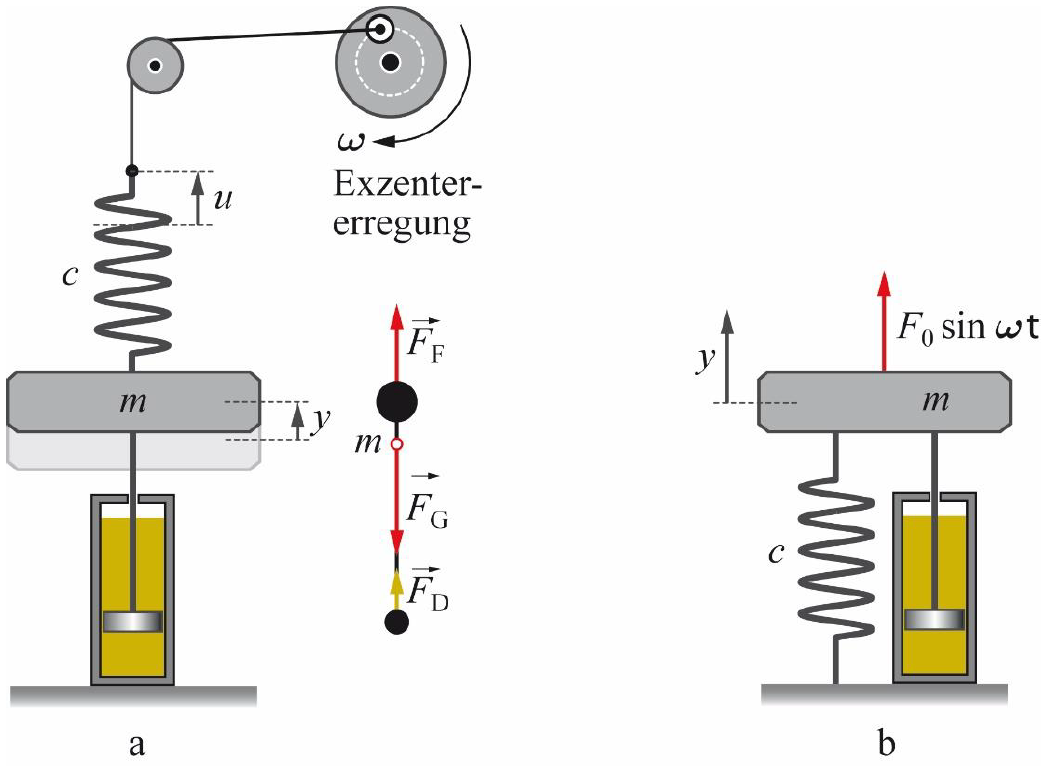
\includegraphics[width=0.75\columnwidth]{images/krafterregung.png}
\end{center}

\vspace{-0.3cm}

$$ \boxed{ \text{DGL:} \quad m \, \ddot{y} + b \, \dot{y} + c \, y = F_0 \, \sin(\omega \, t) } $$  

$$ y(t) = \underbrace{ A(\omega) \, \sin(\omega \, t - \varphi) }_{\substack{y_p(t)}} + \underbrace{ B \, e^{- \delta t} \sin(\Omega_d \, t + \varphi_0)}_{\substack{y_h(t)}} $$


\begin{minipage}[c]{0.3\columnwidth}
    $$ \boxed{ \varphi = \arctan \left( \frac{2 \, D \, \omega_0 \, \omega}{\omega_0^2 - \omega^2} \right) } $$
\end{minipage}
\hfill
\begin{minipage}[c]{0.68\columnwidth}
    $$ \boxed{ A(\omega) = \frac{F_0}{m \sqrt{(\omega_0^2 - \omega^2)^2 + (2 \, D \, \omega_0 \, \omega)^2 } } } $$
\end{minipage}


\subsubsection{Vergrösserungsfunktion / Phasenverschiebung}
\label{Vergrösserungsfunktion / Phasenverschiebung}

\vspace{-0.2cm}

\[
    \boxed{ V = \frac{1}{\sqrt{(1- \eta^2)^2 + (2 \, D \, \eta)^2} } }
    \qquad \qquad
    \boxed{ \varphi = \arctan \left( \frac{2 \, D \, \eta}{1 - \eta^2}  \right) }
\]
$$ \boxed{ V_r = \frac{1}{\sqrt{ 1 - \eta_r^4} } \qquad \text{mit } \eta_r = \sqrt{1 - 2 \, D^2} } $$


\begin{ctabular}{c l c}
    $\varphi$   & Phasenverschiebung                    & $[ \varphi] = \rad$                   \\
    $V$         & Vergrösserungsfunktion                & $[V] = 1$                             \\
    $V_r$       & Vergrösserungsfunktion                & $[V_r] = 1$                           \\
    $\eta$      & Dimensionslose Frequenz               & $[\eta] = 1$                          \\
    $D$         & Dämpfungsgrad                         & $[D] = 1$                             \\
    $A(\omega)$ & Amplitudenverlauf                     & $[A(\omega)] = \meter$                \\
    $\varphi$   & Phasenverschiebung                    & $[\varphi] = \rad$                    \\
    $\omega_0$  & Kreisfrequenz ungedämpfte Schwingung  & $[\omega_0] = \frac{\rad}{\second}$   \\
    $\omega$    & Kreisfrequenz der Störung (Erreger)   & $[\omega] = \frac{\rad}{\second}$     \\
\end{ctabular}


\subsection{Fremderregte Schwingungen -- Dämpfererregung}

\begin{minipage}[t]{0.21\columnwidth}
    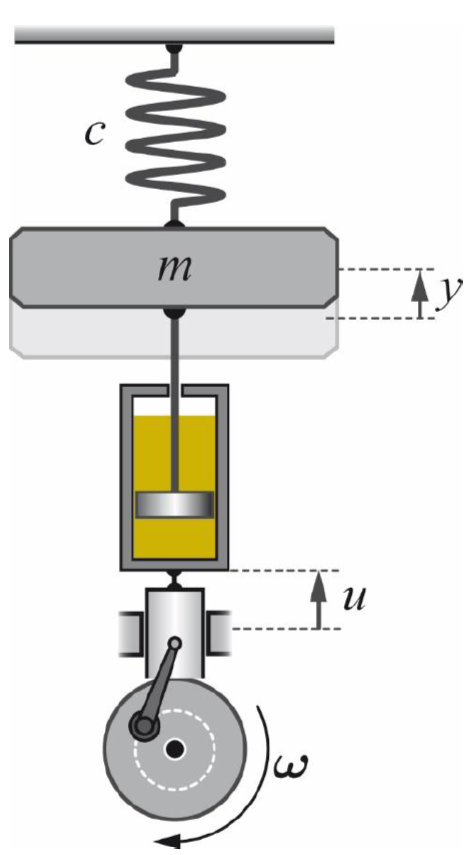
\includegraphics[width=\columnwidth, align=t]{images/daempfererregung.png}
\end{minipage}
\hfill
\begin{minipage}[t]{0.71\columnwidth}
    $$ \boxed{ \text{DGL:} \quad m \, \ddot{y} + b \, \dot{y} + c \, y = b \, \omega  \, u_0 \, \cos(\omega \, t) } $$ 
    $$ A(\omega) =  \frac{b \, \omega \, u_0}{ m \sqrt{(\omega_0^2 -\omega^2)^2 + (2D \omega_0 \omega)^2}} $$ 

    \[
        \boxed{ V = \frac{2 \, D \, \eta}{\sqrt{(1- \eta^2)^2 + (2 \, D \, \eta)^2} } }
        \qquad 
        \boxed{ \varphi = \arctan \left( \frac{2 \, D \, \eta}{1 - \eta^2} \right) - \frac{\pi}{2} }
    \]

    \textrightarrow\ Legende siehe Abschnitt \ref{Vergrösserungsfunktion / Phasenverschiebung}
\end{minipage}


\subsection{Fremderregte Schwingungen -- Stützenerregung}

\begin{minipage}[t]{0.22\columnwidth}
    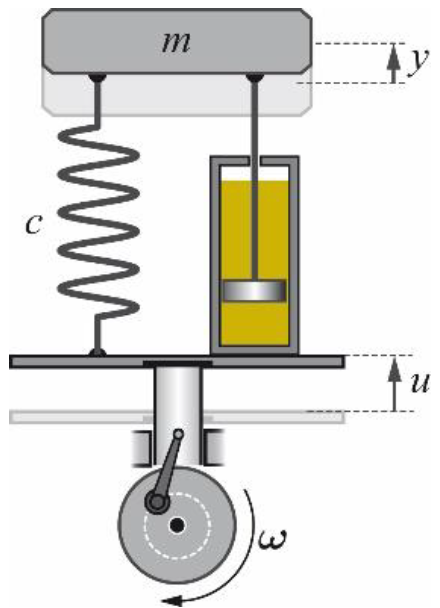
\includegraphics[width=\columnwidth, align=t]{images/stuetzenerregung.png}
\end{minipage}
\hfill
\begin{minipage}[t]{0.7\columnwidth}
    $$ \boxed{ \text{DGL:} \quad m \, \ddot{q} + b \, \dot{q} + c \, q = -m \, \omega^2 \, u_0 \, \sin(\omega \, t)  \quad \text{mit } q = y - u } $$
    $$ A(\omega) = \frac{\omega^2 u_0}{\sqrt{(\omega_0^2 -\omega^2)^2 + (2 \, D \, \omega_0 \, \omega)^2}} $$ 

    \[
        \boxed{ V = \frac{\eta^2}{\sqrt{(1- \eta^2)^2 + (2 \, D \, \eta)^2} } }
        \qquad 
        \boxed{ \varphi = \arctan \left( \frac{2 \, D \, \eta}{1 - \eta^2} \right) - \pi }
    \]

    \textrightarrow\ Legende siehe Abschnitt \ref{Vergrösserungsfunktion / Phasenverschiebung}
\end{minipage}



\subsection{Fremderregte Schwingung -- Unwuchterregung}
\textbf{Unwucht:} Schwerpunkt $S$ des Rotors der Masse $m_R$ bewegt sich auf einem Kreis mit\\
Radius $e$

\begin{minipage}[t]{0.52\columnwidth}
    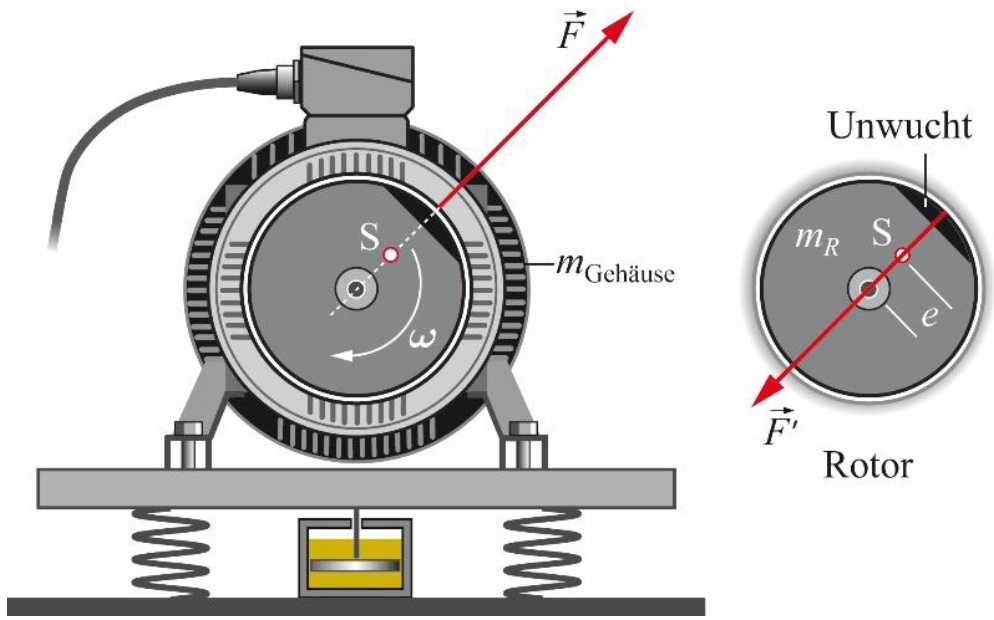
\includegraphics[height=3cm, align=t]{images/unwucht.png}
\end{minipage}
\hfill
\begin{minipage}[t]{0.44\columnwidth}
    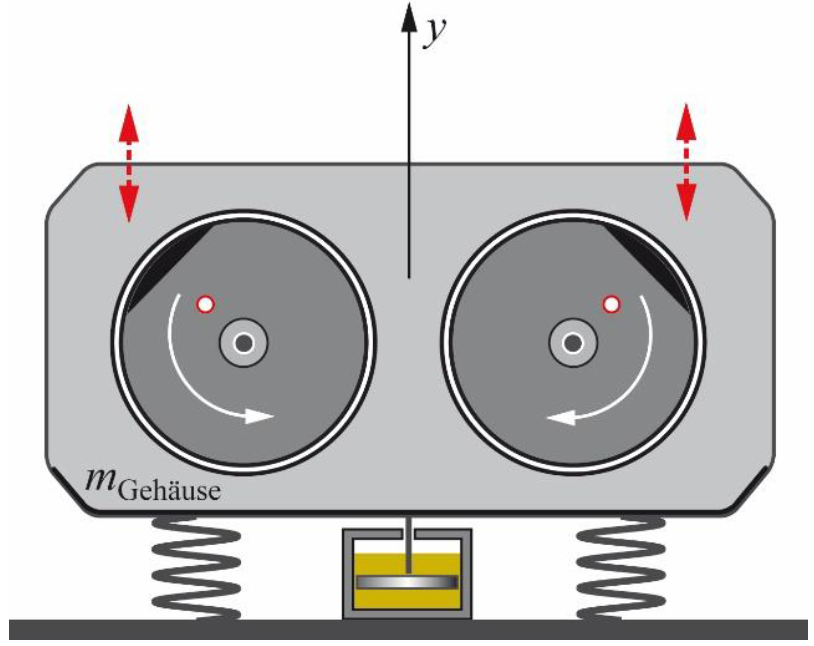
\includegraphics[height=3cm, align=t]{images/unwucht_gehause.png}
\end{minipage}

\smallskip

$$ \boxed{ \text{DGL in y-Richtung:} \quad m \ddot{y} + b \dot{y} + c \, y = -m_R \, \omega^2 \, e \, \sin(\omega \, t) }  $$

\renewcommand{\arraystretch}{1,7}
\begin{tabular}{ll}
    Radiale Beschleunigung des Schwerpunkts des Rotors: & $a_R = \omega^2 e$                                    \\
    Kraft des Rotors auf die Maschine:                  & $\boxed{ F_U = m_R \cdot a_R = m_R \cdot \omega^2 e }$ 
\end{tabular}
\renewcommand{\arraystretch}{1}

\medskip

\[
    A(\omega) = \frac{m_R}{m} \frac{e \, \omega^2}{\sqrt{(\omega_0^2 -\omega^2)^2 + (2 \, D \, \omega_0 \, \omega)^2}} 
    \qquad \qquad
    A_R = \frac{m_R}{m} \frac{e}{2 \, D \sqrt{1 - D^2}}
\]


\subsubsection{Kraft auf die Basis des Gehäuses} 

\vspace{-0.5cm}

\[
    F_B = c y + b \dot{y} = F_{B0} \sin(\omega t - \varphi + \psi)
    \qquad 
    \varphi = \psi - \pi
    \qquad 
    \boxed{ F_{B0} = \frac{m_R \, e \, \omega^2 \sqrt{1+ (2D \eta)^2}}{\sqrt{(1 - \eta^2)^2 + (2 D \eta)^2}} }
\]


\begin{ctabular}{c l c}
    $F_{B0}$    & Kraft auf Basis des Gehäuses          & $[F_{B0}] = \newton$              \\
    $m_R$       & Masse des Rotors                      & $[m_R] = \kilogram$               \\
    $a_R$       & Radiale Beschleinigung Schwerpunkt    & $[a_R] = \frac{\meter}{\second}$  \\
    $e$         & Abstand Mittelpunkt - Schwerpunkt     & $[e] = \meter$                    \\
    $\varphi$   & Phasenverschiebung                    & $[ \varphi] = \rad$               \\
    $V$         & Vergrösserungsfunktion                & $[V] = 1$                         \\
    $\eta$      & Dimensionslose Frequenz               & $[\eta] = 1$                      \\
    $D$         & Dämpfungsgrad                         & $[D] = 1$                         \\
    $A(\omega)$ & Amplitude                             & $[A(\omega)] = \meter$            \\
    $A_R$       & Resonanzamplitude                     & $[A_R] = \meter$
\end{ctabular}


\subsection{Fremderregte Schwingung -- Schwingkreis}

\begin{minipage}[t]{0.4\columnwidth}
    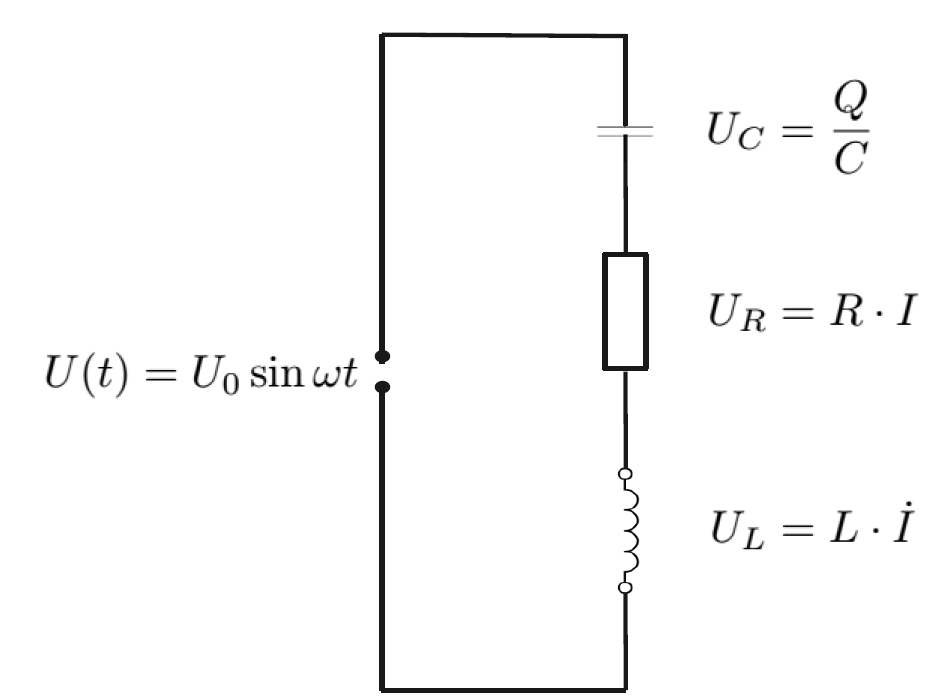
\includegraphics[width=\columnwidth, align=t]{images/schwingkreis.png}
\end{minipage}
\hfill
\begin{minipage}[t]{0.58\columnwidth}
    $$ \boxed{ \text{DGL:} \quad L \ddot{I} + R \dot{I} + \frac{1}{C} \, I = \omega \, U_0 \,\sin \left( \omega \, t + \frac{\pi}{2} \right) } $$
    \textrightarrow\  Gleiche DGL wie bei \cbl{Dämpfererregung}

    $$ \cbl{\text{DGL:} \quad m \ddot{y} + b \dot{y} + c \, y = b \, \omega \, u_0 \, \cos(\omega \, t) } $$
    $$ \cbl{A(\omega) =  \frac{b \, \omega \, u_0}{m \sqrt{(\omega_0^2 -\omega^2)^2 + (2 \, D \, \omega_0 \, \omega)^2}} } $$
\end{minipage}

\medskip

$$ \boxed{ I(\omega) =  \frac{\omega}{\sqrt{(\omega_0^2 -\omega^2)^2 + (2 \, D \, \omega_0 \, \omega)^2}} U_0 \qquad \text{mit} \quad \omega_0 = \frac{1}{\sqrt{LC}} , \quad D = \frac{R}{2}\sqrt{\frac{C}{L}}} $$ 
\[
    \boxed{ V = \frac{U_{L0}}{U_0} = \frac{\eta^2}{\sqrt{(1 - \eta^2)^2 + (2 \, D \, \eta)^2}} }
    \qquad 
    \boxed{ \varphi = \arctan \left( \frac{2 \, D \, \eta}{1 - \eta^2} \right) - \pi }
\]


\subsubsection{Resonanz}

\begin{minipage}{0.48\columnwidth}
    \paragraph{Resonanzfrequenz}
    $$ \boxed{ \omega_r = \omega_0 = \frac{1}{\sqrt{LC}} } $$ 
\end{minipage}
\hfill
\begin{minipage}{0.48\columnwidth}
    \paragraph{Amplitude @ Resonanz}
    $$ \boxed{ I_{0r} = \frac{U_0}{R} } $$ 
\end{minipage}

\renewcommand{\arraystretch}{1.3}
\begin{ctabular}{c l c}
    $\omega_0$  & Kreisfrequenz ungedämpfte Schwingung  & $[\omega_0] = \frac{\rad}{\second}$   \\
    $\omega$    & Kreisfrequenz der Störung (Erreger)   & $[\omega] = \frac{\rad}{\second}$     \\
    $\omega_r$  & Resonanzfrequenz                      & $[\omega_r] = \frac{\rad}{\second}$   \\
    $I_{0r}$    & Strom-Amplitude @ Resonanz            & $[I_{0r}] = \ampere$                  \\
    $U_0$       & Amplitude der Erregerspannung         & $[U_0] = \volt$                       \\
    $U_{L0}$    & Amplitude Spulenspannung              & $[U_{L0}] = \volt$                    \\
    $A(\omega)$ & Amplitude der Schwingung              & $[A(\omega)] = \meter$                \\
    $V$         & Vergrösserungsfunktion                & $[V] = 1$                             \\
    $\eta$      & Dimensionslose Frequenz               & $[\eta] = 1$                          \\
    $D$         & Dämpfungsgrad                         & $[D] = 1$ 
\end{ctabular}
\renewcommand{\arraystretch}{1}


\subsection[Fremderregte Schwingung -- Güte]{Fremderregte Schwingung -- Güte $Q$}

\subsubsection{Definition}

\begin{minipage}[c]{0.48\columnwidth}
    Die relative Abnahme der Schwingungsenergie $E(t)$ pro Schwingdauer wird als \textbf{Güte} oder \textbf{Gütefaktor} bezeichnet.
\end{minipage}
\hfill
\begin{minipage}[c]{0.48\columnwidth}
    $$ \boxed{ Q = 2 \pi \frac{E(t)}{E(t) - E(t + T)} } $$ 
\end{minipage}


\subsubsection{Beziehungen}

\begin{minipage}[t]{0.36\columnwidth}
    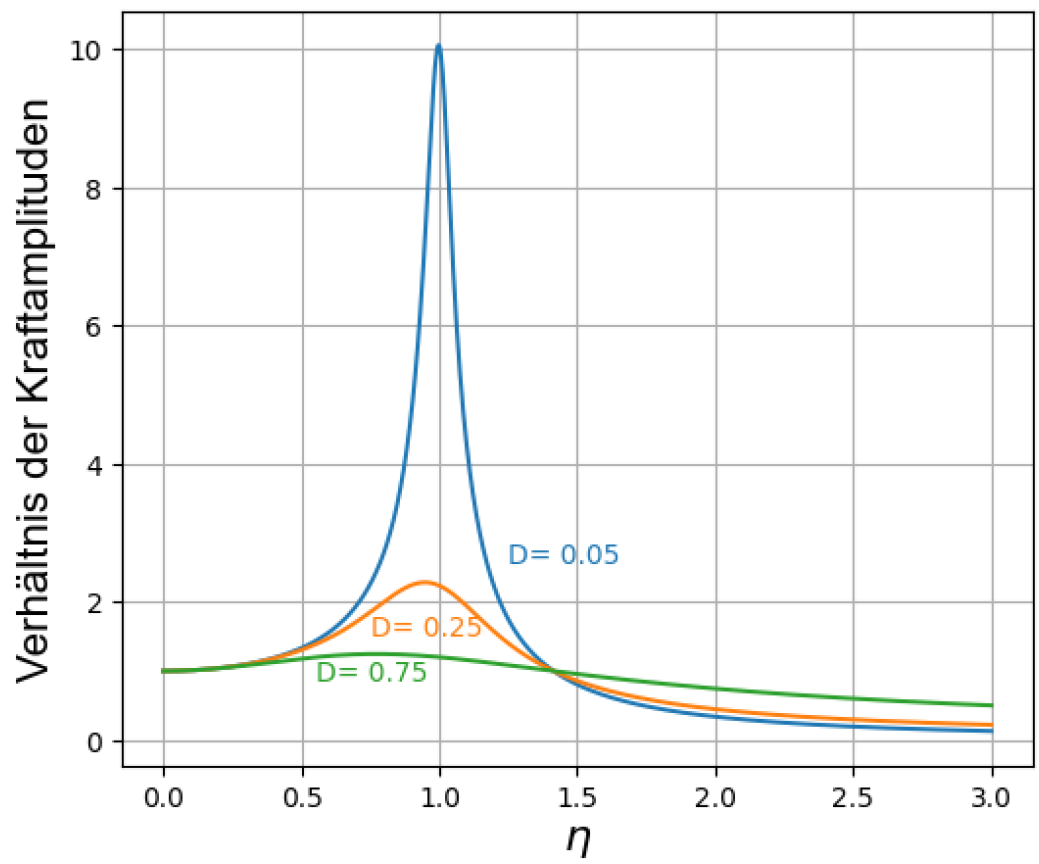
\includegraphics[width=\columnwidth, align=t]{images/guete_resonanz.png}
\end{minipage}
\hfill
\begin{minipage}[t]{0.58\columnwidth}
    \[
        \boxed{Q = \frac{1}{2 \, D} } 
        \qquad \qquad 
        \boxed{ Q = \frac{\omega_0}{\Delta \omega} }
    \]


    \medskip
    Breite der Resonanzkurve bei $U_0 = \frac{U_{0r}}{\sqrt{2}}$ \\
    \textbf{Breite Kurve \textrightarrow\  tiefe Güte}
\end{minipage}


\subsection{Gekoppelte Pendel}
Zwei Pendel sind durch eine Feder miteinander verbunden.

\textbf{Die Bewegung eines Pendels hat Auswirkungen auf die Bewegung des anderen Pendles.}
Gesucht ist eine Berschreibung der Bewegung des Pendels.

\medskip

\begin{minipage}[t]{0.28\columnwidth}
    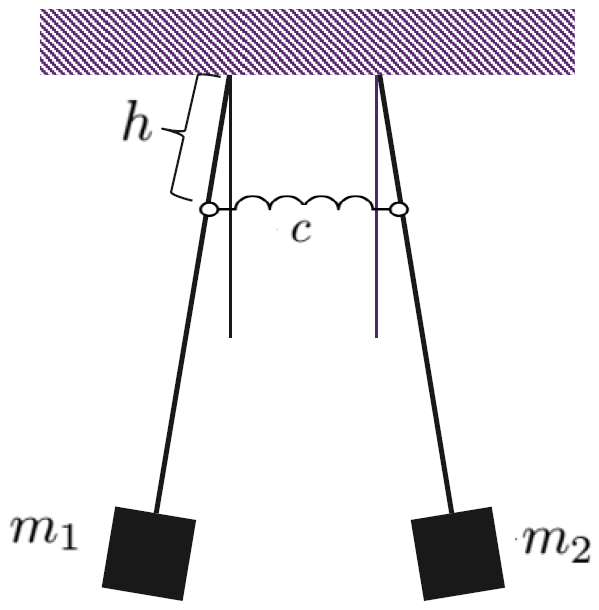
\includegraphics[width=\columnwidth, align=t]{images/gekoppelte_pendel.png}
\end{minipage}
\hfill
\begin{minipage}[t]{0.7\columnwidth}
    \paragraph{Allgemein}

    \vspace{-0.2cm}
    $$ J_1 \ddot{\varphi_1} = -m_1 \, g \, a_1 \, \varphi_1 + c \cdot h^2 \, (\varphi_2 - \varphi_1) $$
    $$ J_2 \ddot{\varphi_2} = -m_2 \, g \,  a_2 \, \varphi_2 - c \cdot h^2 \, (\varphi_2 - \varphi_1) $$

    \medskip

    \paragraph{Spezialfall}

    \begin{tabular}{lll}
        \tabitem $J_1 = J_2 = J$    & \tabitem $m_1 = m_2 = m$  & \tabitem $a_1 = a_2 = a$  \\
    \end{tabular}

    $$ \ddot{\varphi_1} = - \omega^2 \varphi_1 + k \, (\varphi_2 - \varphi_1) $$
    $$ \ddot{\varphi_2} = - \omega^2 \varphi_2 - k \, (\varphi_2 - \varphi_1) $$ 
\end{minipage}

Im Spezialfall gilt:

\vspace{-0.2cm}

\renewcommand{\arraystretch}{2}
\begin{ctabular}{lll}
    $\Phi_+ = \varphi_1 + \varphi_2$    & $\Phi_- = \varphi_2 - \varphi_1$  &                                       \\
    $\omega^2 = \dfrac{m \, g \, a}{J}$ & $k = \dfrac{c \cdot h^2}{J}$      & $\omega_k = \sqrt{\omega^2 + 2 \, k}$ \\
\end{ctabular}


\begin{ctabular}{l ll l}
    Symm:       & $\ddot{\Phi_+} = - \omega^2 \Phi_+$           & & $\varphi_1(t) = \varphi_2(t) = \dfrac{\Phi_0}{2} \cos \left( \omega t \right)$      \\
    Antisymm:   & $\ddot{\Phi_-} = - (\omega^2 + 2k) \Phi_-$    & & $\varphi_1(t) = -\varphi_2(t) = \dfrac{\Phi_0}{2} \cos \left( \omega_k t \right)$
\end{ctabular}


\subsubsection{Allgemeine Lösung des gekoppelten Systems}

\textrightarrow\ Linearkombination der symmetrischen und asymmetrischen Lösung

\vspace{-0.2cm}

\renewcommand{\arraystretch}{1.8}
\begin{ctabular}{lll}
    $\varphi_1(t) = \Phi \, \sin \left( \Omega\, t \right) \cdot \cos \left( \overline{\omega} \, t \right)$    & & $\Omega = \dfrac{\omega_k - \omega}{2}$             \\
    $\varphi_2(t) = \Phi \, \cos \left( \Omega\, t \right) \cdot \sin \left( \overline{\omega} \, t \right)$    & & $\overline{\omega} = \dfrac{\omega + \omega_k}{2}$
\end{ctabular}
\renewcommand{\arraystretch}{1}


\begin{ctabular}{c l c}
    $k$ & Kopplungsfaktor           & $[k] = 1$                                 \\
    $h$ & Abstand zur Aufhängung    & $[h] = \meter$                            \\
    $J$ & Massenträgheitsmoment     & $[J] = \kilogram \cdot \meter\squared $   \\
    $c$ & Federkonstante            & $[c] = \frac{\newton}{\meter}$
\end{ctabular}


        
        \columnbreak

        \part{Wellen}
		\section{Wellen}

\subsection{Definition}

Eine Welle ist eine \textbf{Störung} eines \textbf{Gleichgewichtszustands}, die sich \textbf{im Raum ausbreitet}.


\subsubsection{Bemerkungen zur Definition}

\begin{outline}
    \1 Voraussetzung für \textbf{Ausbreitung} einer Welle ist \textbf{Kopplung} benachbarter Teilchen
    \1 Störung kann von ganz unterschiedlicher Natur sein: 
        \2 Druck in Luft
		\2 Auslenkung einer Position entlang einem Seil (Saite)
		\2 Eletrische Signale  
\end{outline}

\smallskip

\textbf{ \textrightarrow\ Die Störung wird mit $\bm{\xi}$ beschrieben:} $\bm{\xi = \xi(x, y, z, t)}$ 



\subsection{Klassifizierung von Wellen}

\begin{minipage}[t]{0.5\columnwidth}
    \paragraph{Transversalwellen}

    Welle breitet sich \textbf{senkrecht} zur Störung aus

    \begin{center}
        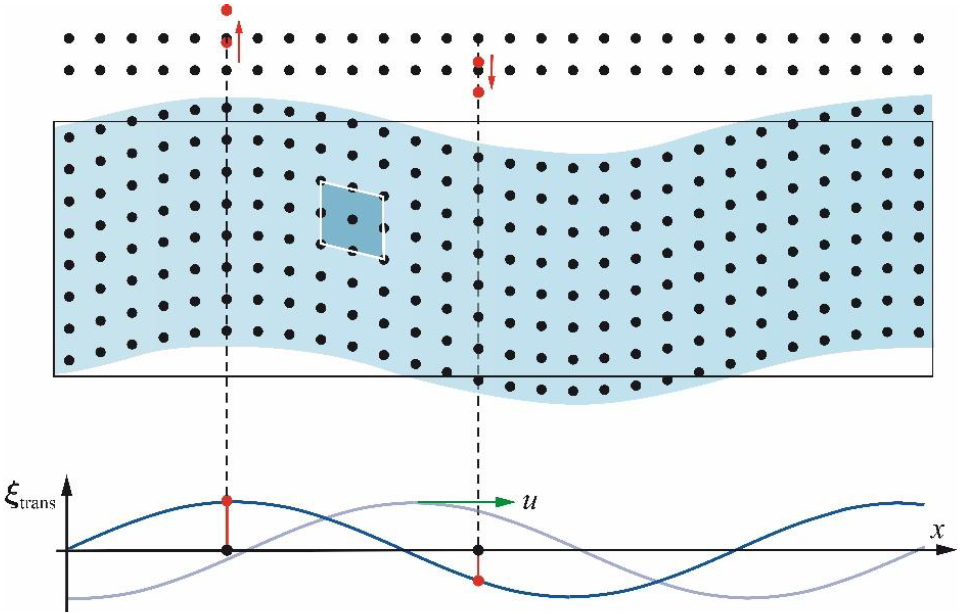
\includegraphics[height=2.6cm, align=t]{images/welle_transversal.png}
    \end{center}
    
    \textbf{Beispiel: } Lichtwellen
\end{minipage}
\hfill
\begin{minipage}[t]{0.48\columnwidth}
    \paragraph{Longitudinalwellen}

    Welle breitet sich \textbf{parallel} zur Störung aus

    \begin{center}
        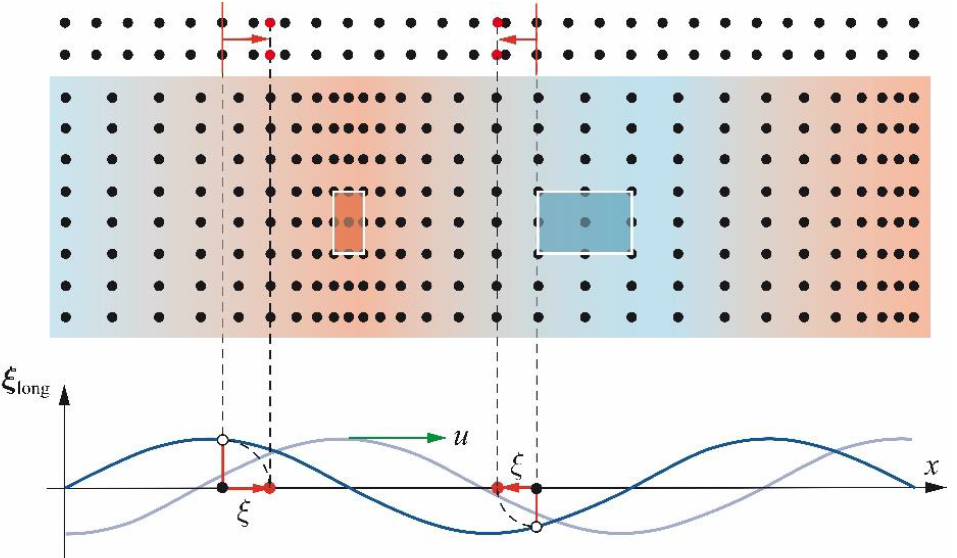
\includegraphics[height=2.6cm, align=t]{images/welle_longitudinal.png}
    \end{center}
    
    \textbf{Beispiel: } Schallwellen
\end{minipage}


\subsection[Wellengeschwindigkeit / Phasengeschwindigkeit]{Wellengeschwindigkeit / Phasengeschwindigkeit $\bm{u}$}

Die Störung an der Position $x_0$ zum Zeitpunkt $t=0$ breitet sich mit der Geschwindigkeit $u$ aus und erreicht nach einer Zeit $t$ die Position $x$

\begin{center}
    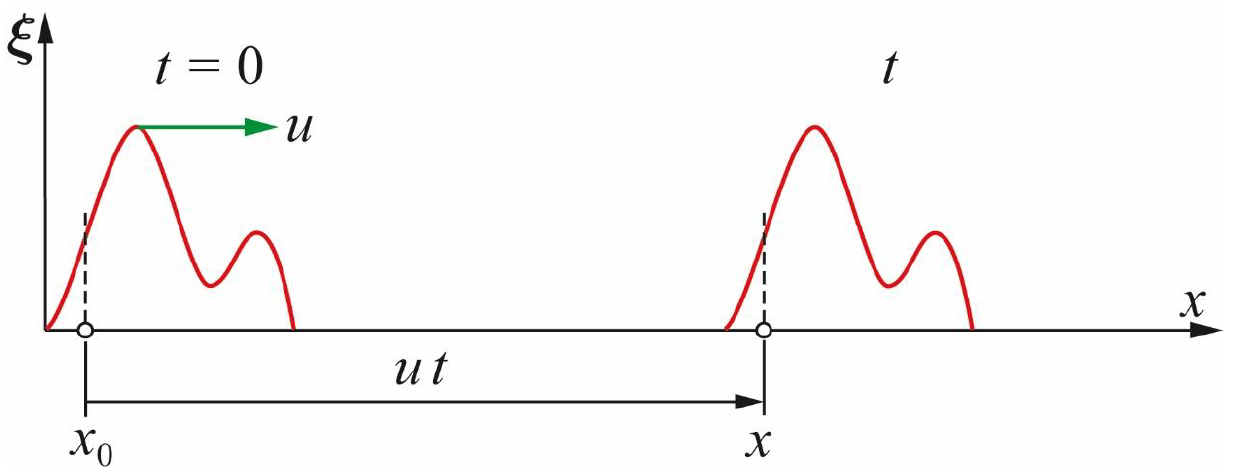
\includegraphics[width=0.62\columnwidth]{images/ausbreitung_stoerung.png}
\end{center}

\vspace{-0.4cm}

$$ \xi(x, t) = \xi(x - ut, 0) = f(x - ut) $$

\smallskip

\textbf{In einem Medium mit grösserer Dichte breiten sich Wellen schneller aus!} \\
\textrightarrow\ Bessere Kopplung der Moleküle

\smallskip

Man schaut bei der Beschreibung der Fortbewegung auf den Ort. Die Verschiebung des Ortes wird mit der Zeit hineingebracht.


\subsubsection{Verschiedene Wellengeschwindigkeiten}

\begin{minipage}{0.45\columnwidth}
    Schallwellen in Fluiden
\end{minipage}
\hfill
\begin{minipage}{0.48\columnwidth}
    $$\boxed{ u = \sqrt{\frac{1}{\rho \, \kappa}} }$$
\end{minipage}

\begin{minipage}{0.45\columnwidth}
    Schallwellen in Gasen
\end{minipage}
\hfill
\begin{minipage}{0.48\columnwidth}
    $$\boxed{ u = \sqrt{\frac{\varkappa \, p}{\rho}} = \sqrt{\frac{\varkappa \, R \, T}{M}} }$$
\end{minipage}

\begin{minipage}{0.45\columnwidth}
    Elastische Longitudinalwellen in einem schlanken Stab
\end{minipage}
\hfill
\begin{minipage}{0.48\columnwidth}
    $$\boxed{ u = \sqrt{\frac{E}{\rho}} }$$
\end{minipage}

\begin{minipage}{0.45\columnwidth}
    Elastische Transversalwellen
\end{minipage}
\hfill
\begin{minipage}{0.48\columnwidth}
    $$\boxed{ u = \sqrt{\frac{G}{\rho}} }$$
\end{minipage}

\begin{minipage}{0.45\columnwidth}
    Transversalwellen auf einem Seil oder einer Saite
\end{minipage}
\hfill
\begin{minipage}{0.48\columnwidth}
    $$\boxed{ u = \sqrt{\frac{F}{\rho \, A}} }$$ 
\end{minipage}

\begin{minipage}{0.45\columnwidth}
    Elektromagnetische Wellen (transversal) \\
    (z.B. Lichtwellen)
\end{minipage}
\hfill
\begin{minipage}{0.48\columnwidth}
    $$\boxed{ u = \frac{c}{n} }$$
\end{minipage}


\renewcommand{\arraystretch}{1.15}
\begin{ctabular}{c l c}
    $u$         & Wellengeschwindigkeit                                                 & $[u] = \frac{\meter}{\second}$                    \\
    $A$         & Querschnittsfläche                                                    & $[A] = \meter\squared$                            \\
    $E$         & Elastizitätsmodul                                                     & $[E] = \frac{\newton}{\meter\squared} = \pascal$  \\
    $F$         & Spannkraft des Seils / der Saite                                      & $[F] = \newton$                                   \\
    $G$         & Schubmodul                                                            & $[G] = \frac{\newton}{\meter\squared} = \pascal$  \\
    $M$         & Molmasse                                                              & $[M] = \frac{\kilogram}{\mole}$                   \\
    $p$         & Druck                                                                 & $[p] = \pascal$                                   \\
    $R$         & Universelle Gaskonstante: $R = 8.314 \mathrm{\frac{J}{mol \cdot K}}$  & $[R] = \mathrm{\frac{J}{mol \cdot K}} $           \\
    $T$         & \textbf{Absolut-}Temperatur                                           & $[T] = \mathrm{K}$                                \\
    $\kappa$    & Kompressibilität                                                      & $[\kappa] = \frac{1}{\pascal}$                    \\
    $\varkappa$ & Adiabatenexponent                                                     & $[\varkappa] = 1$                                 \\
    $\rho$      & Dichte                                                                & $[\rho] = \frac{\kilogram}{\meter\cubed}$         \\
    $n$         & Brechungsindex                                                        & $[n] = 1$                                         \\
    $c$         & Lichtgeschwindigkeit: $c = 300 \cdot 10^6 \, \frac{\meter}{\second}$  & $[c] = \frac{\meter}{\second}$
\end{ctabular}
\renewcommand{\arraystretch}{1}


\subsection{Wellengleichungen}

Die Wellengleichungen stellen eine \textbf{Verbindung zwischen Zeit und Ort} her.

\medskip
\begin{minipage}{0.45\columnwidth}
    Eindimensional \\
    Welle breitet sich in 1D aus
\end{minipage}
\hfill
\begin{minipage}{0.48\columnwidth}
    $$\boxed{ \frac{\partial^2 \xi}{\partial x^2} = \frac{1}{u^2} \frac{\partial^2 \xi}{\partial t^2}  }$$
\end{minipage}

\begin{minipage}{0.45\columnwidth}
    Zweidimensional \\
    Welle breitet sich in 2D aus
\end{minipage}
\hfill
\begin{minipage}{0.48\columnwidth}
    $$\boxed{ \frac{\partial^2 \xi}{\partial x^2} + \frac{\partial^2 \xi}{\partial y^2} = \frac{1}{u^2} \frac{\partial^2 \xi}{\partial t^2}  }$$
\end{minipage}

\begin{minipage}{0.45\columnwidth}
    Dreidimensional \\
    Welle breitet sich in 3D aus
\end{minipage}
\hfill
\begin{minipage}{0.48\columnwidth}
    $$\boxed{ \frac{\partial^2 \xi}{\partial x^2} + \frac{\partial^2 \xi}{\partial y^2} + \frac{\partial^2 \xi}{\partial z^2} = \frac{1}{u^2} \frac{\partial^2 \xi}{\partial t^2}  }$$
\end{minipage}


\subsubsection{Wichtige Lösung der Wellengleichung (1D)}

\begin{minipage}{0.38\columnwidth}
    $$\frac{\partial^2 \xi}{\partial x^2} = \frac{1}{u^2} \frac{\partial^2 \xi}{\partial t^2} $$
\end{minipage}
\hfill
\begin{minipage}{0.58\columnwidth}
    Ansatz: $\xi(x,t) = \xi_0 \cdot \sin(\omega \, t - k \, x)$
\end{minipage}

$$ \underbrace{- k^2 \, A \, \sin(\omega \, t - k \, x)}_{\substack{\frac{\partial^2 \xi}{\partial x^2} }} = - \frac{1}{u^2} \cdot \underbrace{ \omega^2 \, A \,\sin(\omega \, t - k \, x)}_{\substack{\frac{\partial^2 \xi}{\partial t^2} }}  $$ 

$$ \boxed{ \text{mit Lösung} \quad  u^2 = \frac{\omega^2}{k^2} } $$


\subsection{Harmonische Wellen}

$$ \boxed{ \xi(x, t) = \xi_0 \cdot \sin( \omega \, t - k \, x + \varphi) }  $$


\subsubsection{Terminologie}

\begin{center}
    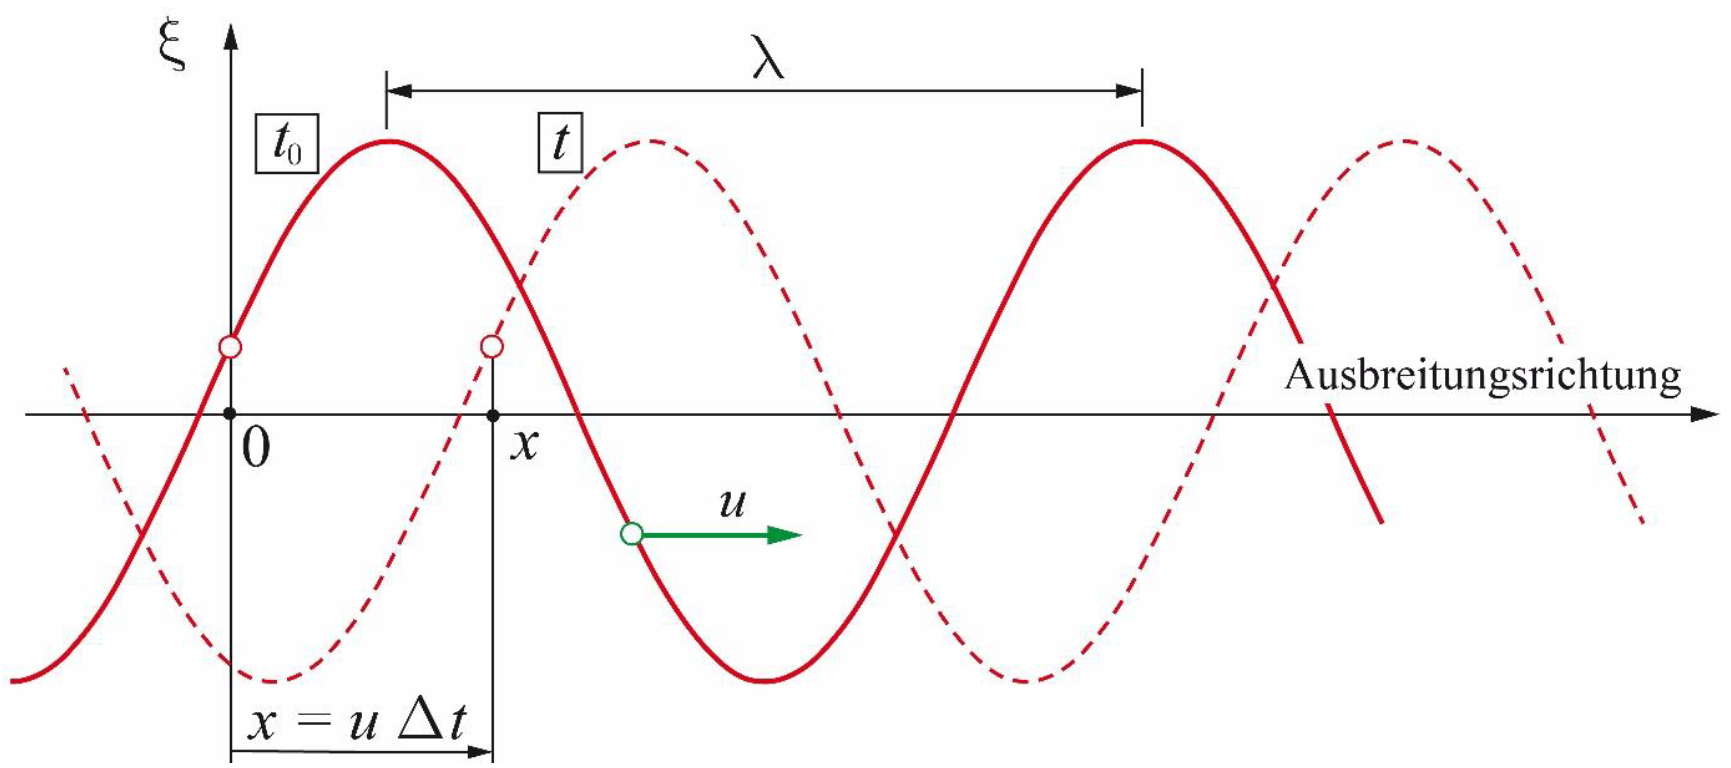
\includegraphics[width=0.7\columnwidth]{images/harmonische_wellen_terminologie.png}
\end{center}

\renewcommand{\arraystretch}{1.2}
\begin{ctabular}{c l c}
    $\xi_0$     & Amplitude             & $[\xi_0]$                         \\
    $\omega$    & Kreisfrequentz        & $[\omega] = \frac{\rad}{\second}$ \\
    $T$         & Periodendauer         & $[T] = \second$                   \\
    $k$         & Wellenzahl            & $[k] = \frac{1}{\meter}$          \\
    $\lambda$   & Wellenlänge           & $\lambda = \meter $               \\
    $u$         & Wellengeschwindigkeit & $[u] = \frac{\meter}{\second}$    \\
    $\varphi$   & Phasenverschiebung    & $[\varphi] = \rad$ 
\end{ctabular}
\renewcommand{\arraystretch}{1}


\subsubsection{Zusammenhänge}

\begin{center}
    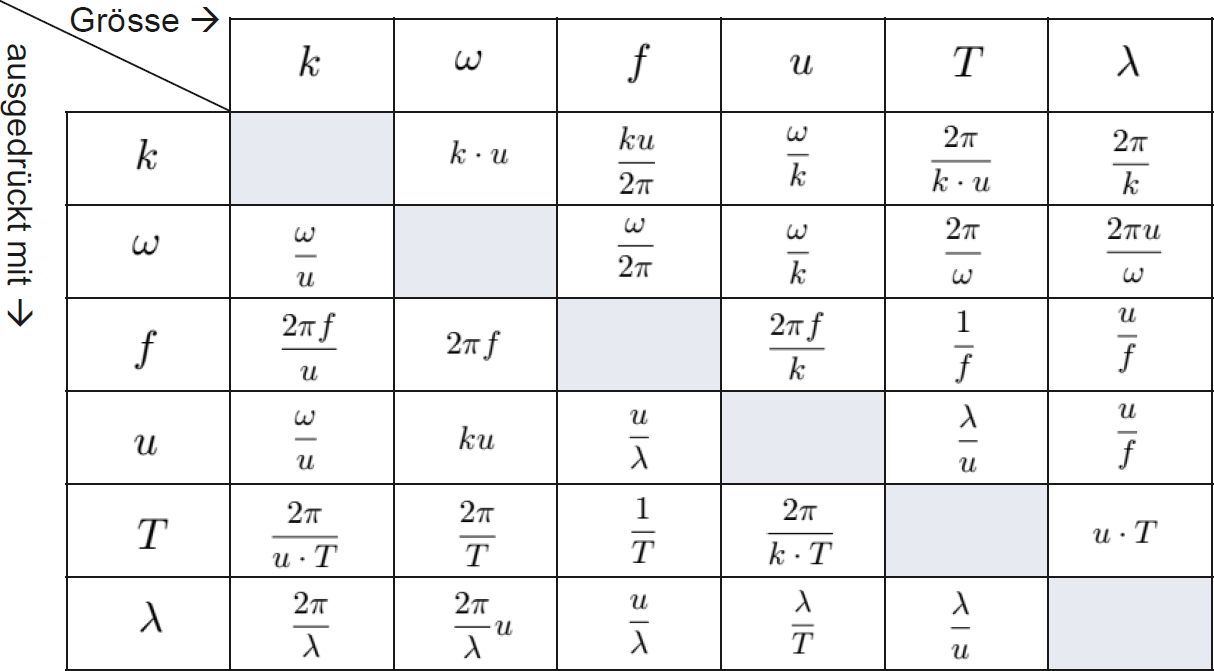
\includegraphics[width=0.9\columnwidth]{images/harmonische_wellen_zusammenhaenge.png}
\end{center}



\subsection{Wellenflächen / Wellenfronten}
Die Gesamtheit aller Punkte, die zu einer bestimmten Zeit im gleichen Schwingungszustand sind, bilden eine Fläche im Raum.

\smallskip

Diese \textbf{Flächen mit gleicher Phase} werden \textbf{Wellenflächen} oder \textbf{Wellenfronten} genannt.

\smallskip

Eine Welle kann sich in 3 Dimensionen ausbreiten und dabei \textbf{verschiedene Wellenflächen} zeigen. 


\subsection{Wellenausbreitung}

\begin{minipage}{0.25\columnwidth}
    Wellengleichung (3D)
\end{minipage}
\hfill
\begin{minipage}{0.73\columnwidth}
    $$\boxed{ \frac{\partial^2 \xi}{\partial x^2} + \frac{\partial^2 \xi}{\partial y^2} + \frac{\partial^2 \xi}{\partial z^2} = \frac{1}{u^2} \frac{\partial^2 \xi}{\partial t^2}  }$$
\end{minipage}

\begin{minipage}{0.25\columnwidth}
    Lösungsansatz
\end{minipage}
\hfill
\begin{minipage}{0.73\columnwidth}
    $$ \boxed{ \xi = \xi_0 e^{\jimg \, (\omega \, t - \vec{k} \bullet \vec{r})} }$$
\end{minipage}

\medskip

mit Wellenvektor $\vec{k} = \begin{pmatrix} k_x \\ k_y \\ k_z  \end{pmatrix}$ und Ortsvektor $ \vec{r} = \begin{pmatrix} r_x \\ r_y \\ r_z  \end{pmatrix}$


\subsubsection{Ebene Wellen}

\begin{minipage}[t]{0.3\columnwidth}
    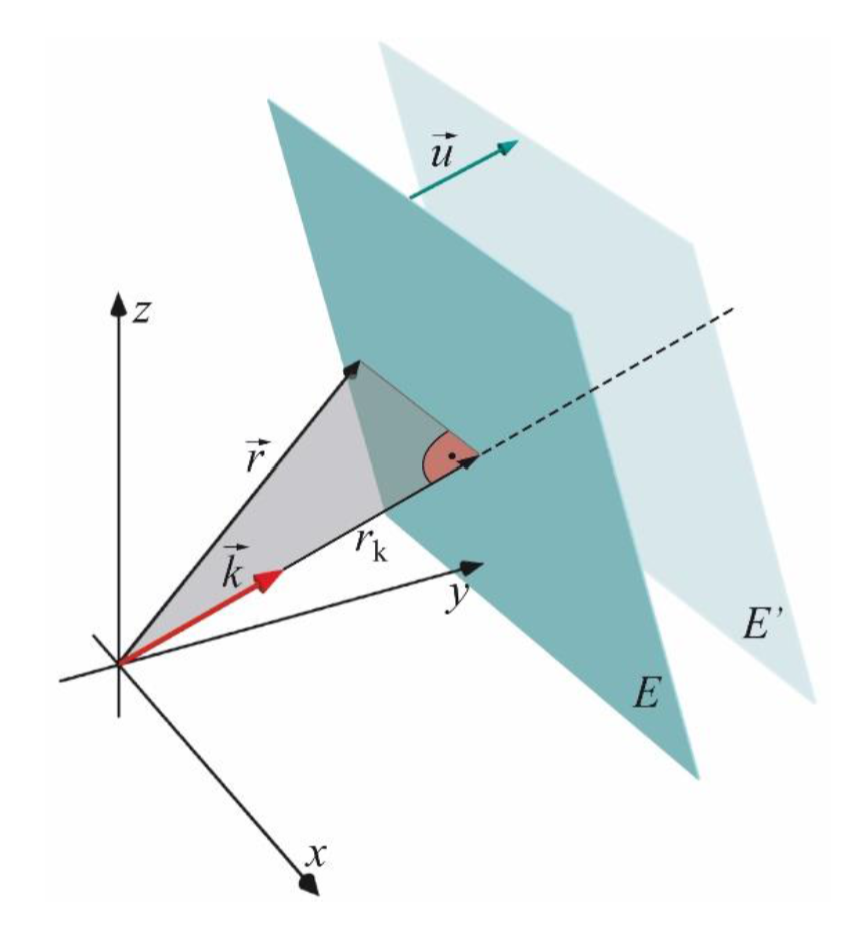
\includegraphics[width=\columnwidth, align=t]{images/Ebene_Welle.png}
\end{minipage}
\hfill
\begin{minipage}[t]{0.68\columnwidth}
    \begin{itemize}
        \item Wellenfronten sind Ebenen im Raum 
        \item Wellenvektor $\vec{k}$ steht senkrecht auf der Ebenen 
        \item \textbf{Abstand} zw. zwei Wellenfronten ist $\lambda$ 
    \end{itemize}

    \medskip

    Die Ebenen bewegen sich mit der Wellengeschwindigkeit
    $$ \boxed{ u = \frac{\omega}{k} \quad \text{ mit } k = ||\vec{k}|| = \sqrt{k_x^2 + k_y^2 + k_z^2} }$$  
    in die \textbf{Richtung}, die durch den \textbf{Wellenvektor} $\vec{k}$ gegeben ist.
\end{minipage}


\subsubsection{Kugelwellen}

\begin{minipage}[t]{0.3\columnwidth}
    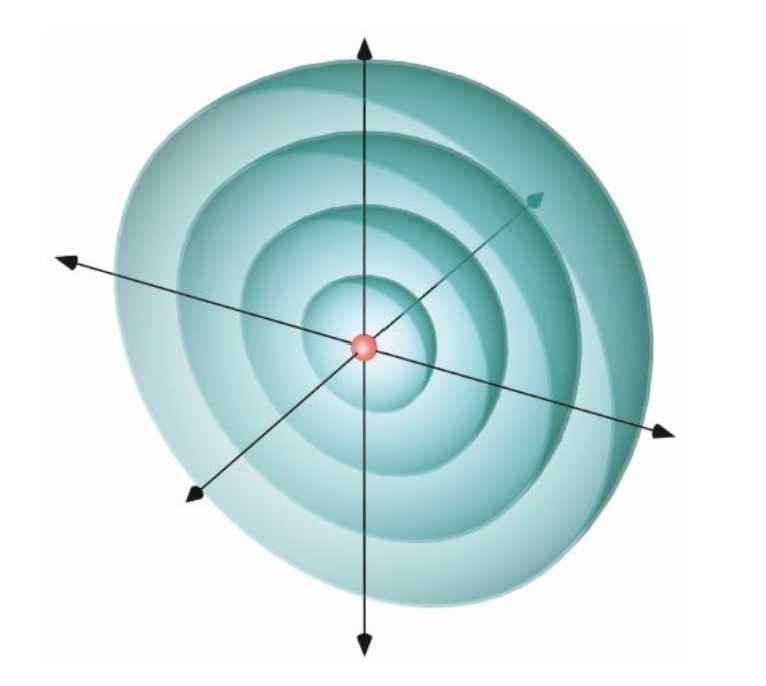
\includegraphics[width=\columnwidth, align=t]{images/Kugel_Welle.png}
\end{minipage}
\hfill
\begin{minipage}[t]{0.68\columnwidth}
    \begin{itemize}
        \item Wellenfronten sind Kugeln 
        \item Wellenvektor $\vec{k}$ steht senkrecht auf Wellenfronten 
        \item Wellenfronten bewegen sich mit der  Wellengeschwindigkeit vom Zentrum weg 
        \item Amplitude nimmt mit $\frac{1}{r}$ ab
    \end{itemize}
\end{minipage}

Für eine \textbf{punktförmige Quelle} und \textbf{keine Winkelabhängigkeit} gilt:

$$ \boxed{ \text{Wellengleichung:} \quad \frac{1}{u^2} \frac{\partial^2 \xi}{\partial t^2} = \frac{2}{r} \left( \frac{\partial \xi}{\partial r} \right) + \frac{\partial^2 \xi}{\partial r^2} }$$

$$ \boxed{ \text{Lösungsansatz:} \quad \xi(t, r) = \frac{1}{r} \xi_0 \, e^{ \jimg \, (\omega \, t - k \, r)} }  $$



\subsection{Bewegte Quellen}

\begin{minipage}[t]{0.46\columnwidth}
    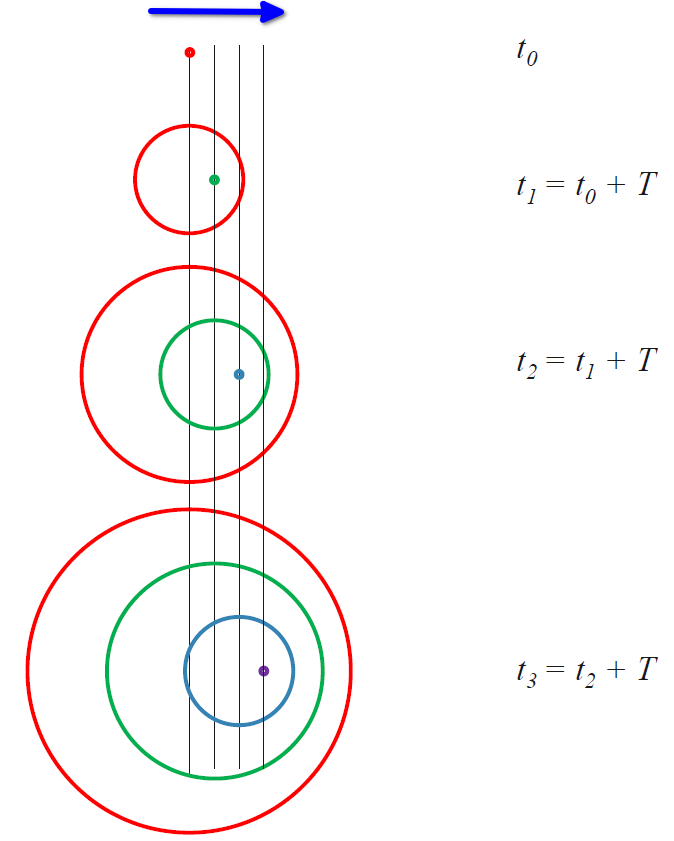
\includegraphics[width=\columnwidth, align=t]{images/Bewegte_Quellen.png}
\end{minipage}
\hfill
\begin{minipage}[t]{0.48\columnwidth}
    Die Quelle bewegt sich mit der \cbl{Geschwindigkeit $v_Q$} in eingezeichneter Richtung fort

    \medskip

    Die Quelle verschiebt sich in der Zeit $T$ um 
    $$ \boxed{ \Delta x = v_Q \cdot T }$$
\end{minipage}


\subsubsection{Frequenzverschiebung durch Bewegung der Quelle}


\begin{minipage}[t]{0.54\columnwidth}
    Die Quelle sendet eine Frequenz $f$ aus.
    Durch die Bewegung der Quelle ändert sich die Wellenlänge $\lambda$ und somit ergibt sich eine neue Frequenz $f'$, welche ein statischer Beobachter wahrnimmt.
    
    \vspace{-0.2cm}

    $$ \boxed{f' = \frac{1}{ \left( 1 \mp \frac{v_Q}{u} \right)}f} $$

    \begin{tabular}{@{}ll@{}}
        $+$ & Quelle bewegt sich vom Beobachter weg \\
        $-$ & Quelle bewegt sich zum Beobachter hin
    \end{tabular}
\end{minipage}
\hfill
\begin{minipage}[t]{0.42\columnwidth}
    \paragraph{Herleitung}

    \vspace{-0.5cm}

    \begin{align*}
        \lambda'    &= \lambda -v_Q \cdot T                         \\
        \lambda'    &= \lambda -v_Q \frac{\lambda}{u}               \\
        \lambda'    &= \lambda \left( 1 - \frac{v_Q}{u} \right)     \\
        f'          &= \frac{u}{\lambda'} = \frac{u}{\lambda \left( 1-\frac{v_Q}{u} \right)} = \frac{f}{ \left( 1-\frac{v_Q}{u} \right)}
    \end{align*}
\end{minipage}


\renewcommand{\arraystretch}{1.2}
\begin{ctabular}{clc}
    $\lambda$   & Wellenlänge der aussendeten Welle     & $[\lambda] = \meter$              \\
    $\lambda'$  & Wellenlänge der wahrgenommenen Welle  & $[\lambda'] = \meter$             \\
    $v_Q$       & Geschwindigkeit der bewegten Quelle   & $[v_Q] = \frac{\meter}{\second}$  \\
    $u$         & Wellengeschwindigkeit                 & $[u] = \frac{\meter}{\second}$    \\
    $f$         & Frequenz der ausgesendeten Wellen     & $[f] = \hertz$                    \\
    $f'$        & Frequenz der wahrgenommenen Wellen    & $[f'] = \hertz$                   \\
    $T$         & Periodendauer (Dauer der Ausbreitung) & $[T] = \second$
\end{ctabular}
\renewcommand{\arraystretch}{1}


\subsubsection{Bewegte Quelle vs. unbewegte Quelle}

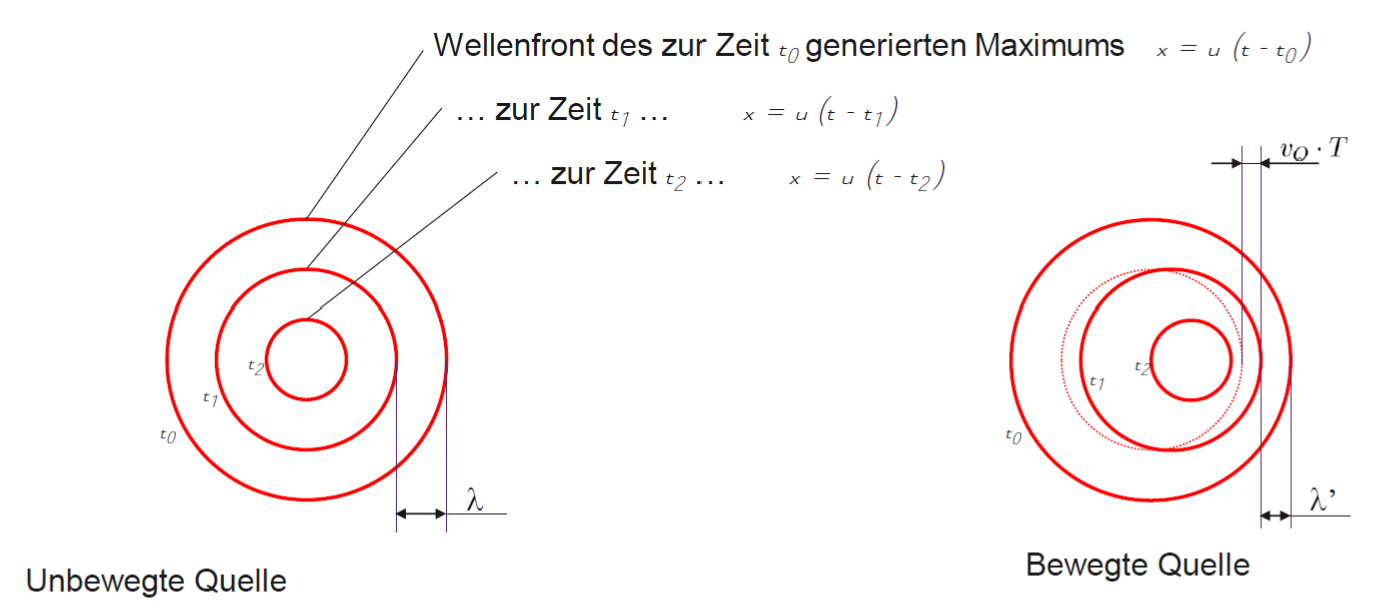
\includegraphics[width=\columnwidth]{images/Unbewegte_Quelle.png}


\subsection{Doppler Effekt}
Die \textbf{Veränderung der Wellenlänge} $\lambda$ der von einer \textbf{bewegten Quelle} ausgesandten Wellen ist als \textbf{Doppler Effekt} bekannt.

\begin{center}
    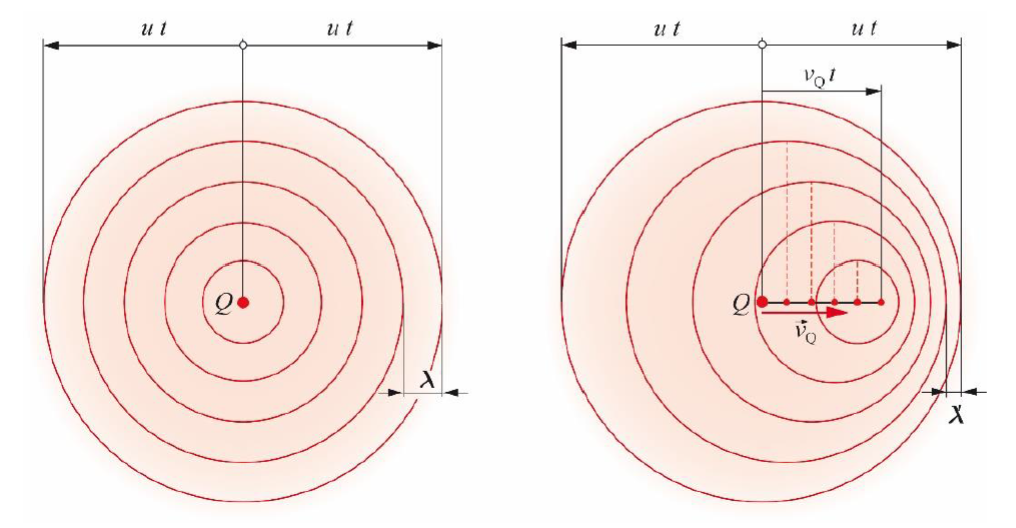
\includegraphics[width=0.8\columnwidth]{images/Doppler_effekt.png}
\end{center}


\subsection{Bewegte Quelle mit Winkel}
Die Quelle bewegt sich nicht direkt auf den Beobachter zu, sondern sie bewegt sich am \textbf{Beobachter vorbei}

\begin{minipage}{0.48\columnwidth}
    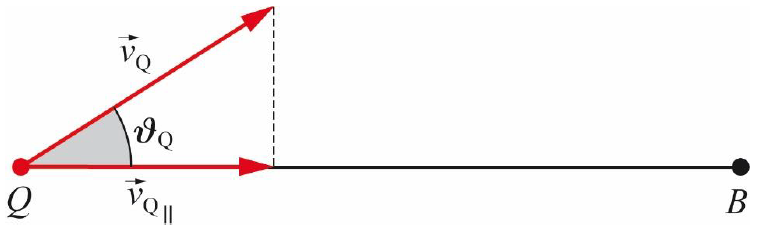
\includegraphics[width=\columnwidth]{images/bewegte_quelle_winkel.png} 
\end{minipage}
\hfill
\begin{minipage}{0.48\columnwidth}
    $$ \boxed{ f' =  \frac{1}{1 - \frac{v_Q}{u} \cdot \cos(v_Q)}  \, f} $$
\end{minipage}

\begin{ctabular}{clc}
    $v_Q$   & Geschwindigkeit der bewegten Quelle   & $[v_Q] = \frac{\meter}{\second}$  \\
    $u$     & Wellengeschwindigkeit                 & $[u] = \frac{\meter}{\second}$    \\
    $f$     & Frequenz der ausgesendeten Wellen     & $[f] = \hertz$                    \\
    $f'$    & Frequenz der wahrgenommenen Wellen    & $[f'] = \hertz$
\end{ctabular}


\subsubsection{Beispiel Winkel zw. Quelle und Beobachter}

\begin{minipage}[t]{0.4\columnwidth}
    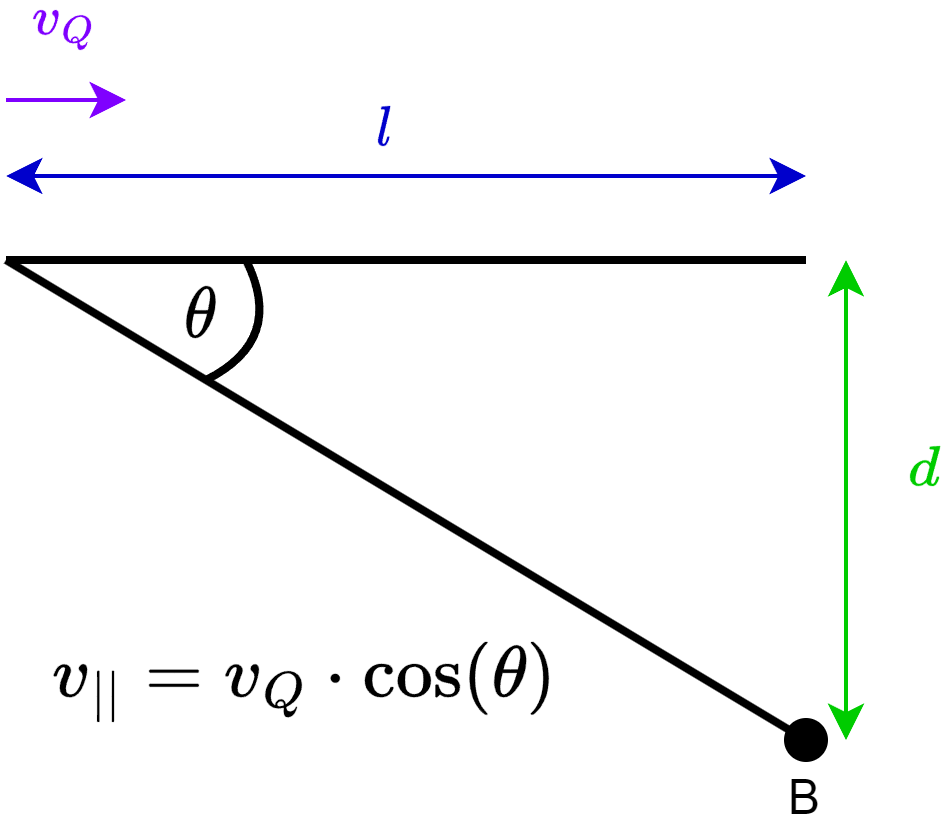
\includegraphics[width=\columnwidth, align=t]{images/beispiel_bewegte_quelle.png} 
\end{minipage}
\hfill
\begin{minipage}[t]{0.58\columnwidth}
    \textbf{Gegeben:} $v_Q, \, \theta, \,u, \,d, \,l$ \qquad 
    \textbf{Gesucht:} $\frac{f'}{f}$
    $$f' =  \frac{1}{1 - \frac{v_Q}{u} \cdot \cos(v_Q)}$$
    \[
        \tan(\theta) = \frac{d}{l} =  \frac{\sin(\theta)}{\cos(\theta)} \qquad
        \sin^2(\theta) = 1 - \cos^2(\theta)
    \]

    $$ \Rightarrow\ \tan(\theta) = \frac{d}{l} = \frac{\sqrt{ 1 - \cos^2(\theta)}}{\cos(\theta)} $$

    \[
        \frac{1}{\cos^2(\theta)} = \frac{d^2}{l^2} + 1  \qquad
        \cos^2(\theta) = \frac{1}{1 + \frac{d^2}{l^2}}
    \]
\end{minipage}

$$ \boxed{ \Rightarrow\ \frac{f'}{f} = \frac{1}{1 - \frac{v_Q}{u} \cdot \sqrt{\frac{l^2}{l^2 + d^2} } } } $$


\subsection{Bewegter Beobachter}

\begin{minipage}[l]{0.48\columnwidth}
    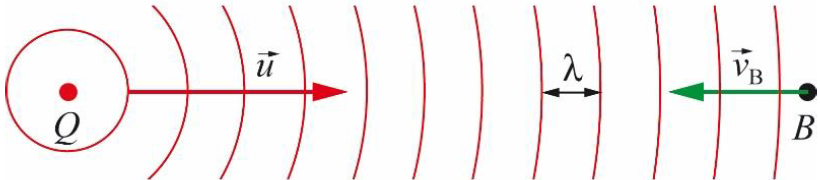
\includegraphics[width=\columnwidth, align=t]{images/bewegter_beobachter.png}
    \end{minipage}
\hfill
\begin{minipage}[l]{0.48\columnwidth}
    $$ \boxed{f' = \left( 1 \pm \frac{v_B}{u}  \right) \, f } $$

    \begin{tabular}{ll}
        $+$ & Beobachter geht auf Quelle zu \\
        $-$ & Beobachter geht von Quelle weg
    \end{tabular}
\end{minipage}


\renewcommand{\arraystretch}{1.2}
\begin{ctabular}{clc}
    $v_B$   & Geschwindigkeit des bewegten Beobachters  & $[v_B] = \frac{\meter}{\second}$  \\
    $v_Q$   & Geschwindigkeit der bewegten Quelle       & $[v_Q] = \frac{\meter}{\second}$  \\
    $u$     & Wellengeschwindigkeit                     & $[u] = \frac{\meter}{\second}$    \\
    $f_B$   & Frequenz, welche Beobachter wahrnimmt     & $[f_B] = \hertz$                  \\
    $f_Q$   & Frequenz, welche Quelle 'aussendet'       & $[f_Q] = \hertz$ 
\end{ctabular}
\renewcommand{\arraystretch}{1}



\subsection{Bewegte Quelle und bewegter Beobachter}

\begin{minipage}[c]{0.48\columnwidth}
    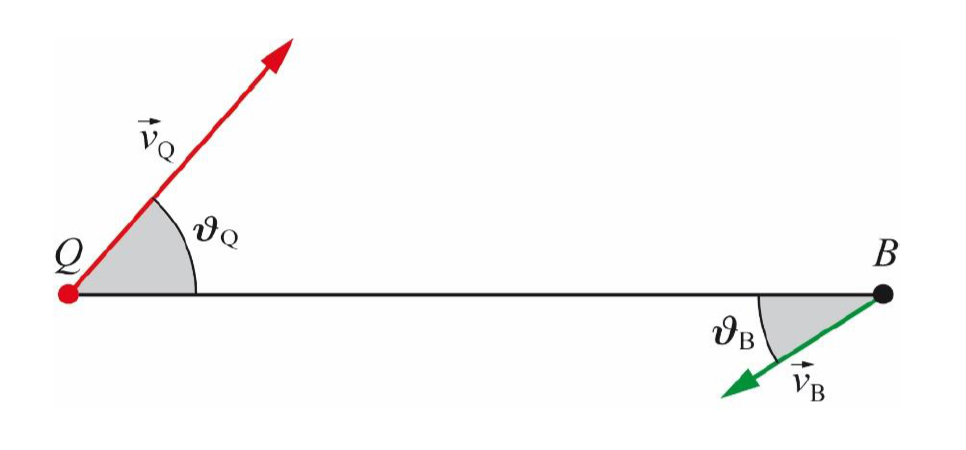
\includegraphics[width=\columnwidth]{images/akustischer_doppler_effekt.png} 
\end{minipage}
\hfill
\begin{minipage}[c]{0.48\columnwidth}
    $$ \boxed{f_B = \frac{u+ v_B \cos(\vartheta_B)}{u- v_Q \cos(\vartheta_Q)}f_Q} $$
\end{minipage}

\renewcommand{\arraystretch}{1.2}
\begin{ctabular}{clc}
    $\vartheta_B = \theta_B$    & siehe Skizze                          & $[\vartheta_B] = \degree$         \\
    $v_B$                       & Geschwindigkeit bewegter Beobachter   & $[v_B] = \frac{\meter}{\second}$  \\
    $\vartheta_Q = \theta_Q$    & siehe Skizze                          & $[\vartheta_Q] = \degree$         \\
    $v_Q$                       & Geschwindigkeit bewegte Quelle        & $[v_Q] = \frac{\meter}{\second}$  \\
    $u$                         & Wellengeschwindigkeit                 & $[u] = \frac{\meter}{\second}$    \\
    $f_B$                       & Frequenz beim bewegten Beobachter     & $[f_B] = \hertz$                  \\
    $f_Q$                       & Frequenz bei der bewegten Quelle      & $[f_Q] = \hertz$
\end{ctabular}
\renewcommand{\arraystretch}{1}


\subsubsection{Optischer Doppler Effekt}

\textbf{Wird verwendet, wenn die Wellengeschwindigkeit $\boldsymbol{u}$ gleich der Lichtgeschwindigkeit $\boldsymbol{c}$ ist!}

Es spielt nur die \textbf{relative} Bewegung von Beobachter und Quellen eine Rolle

$$ \boxed{f' = \frac{\sqrt{1-\beta^2}}{1 - \beta \cos(\vartheta)}f \qquad  \text{ mit} \quad \beta = \frac{v}{c} } $$

\vspace{-0.2cm}

\begin{align*}
    \text{für } \beta \ll 1 \qquad f'                                            &\simeq \frac{1}{1- \beta \cdot \cos(\theta)} \cdot f \\
    \text{für } \beta \ll 1 \text{ und } \theta \approx \frac{\pi}{2} \qquad f'  &\simeq \frac{1}{1- \beta } \cdot f
\end{align*}



\subsubsection{Mach'scher Kegel}

Wenn sich die Quelle schneller fortbewegt als die Wellengeschwindigkeit, dann entsteht ein Mach'scher Kegel

\begin{minipage}[t]{0.6\columnwidth}
    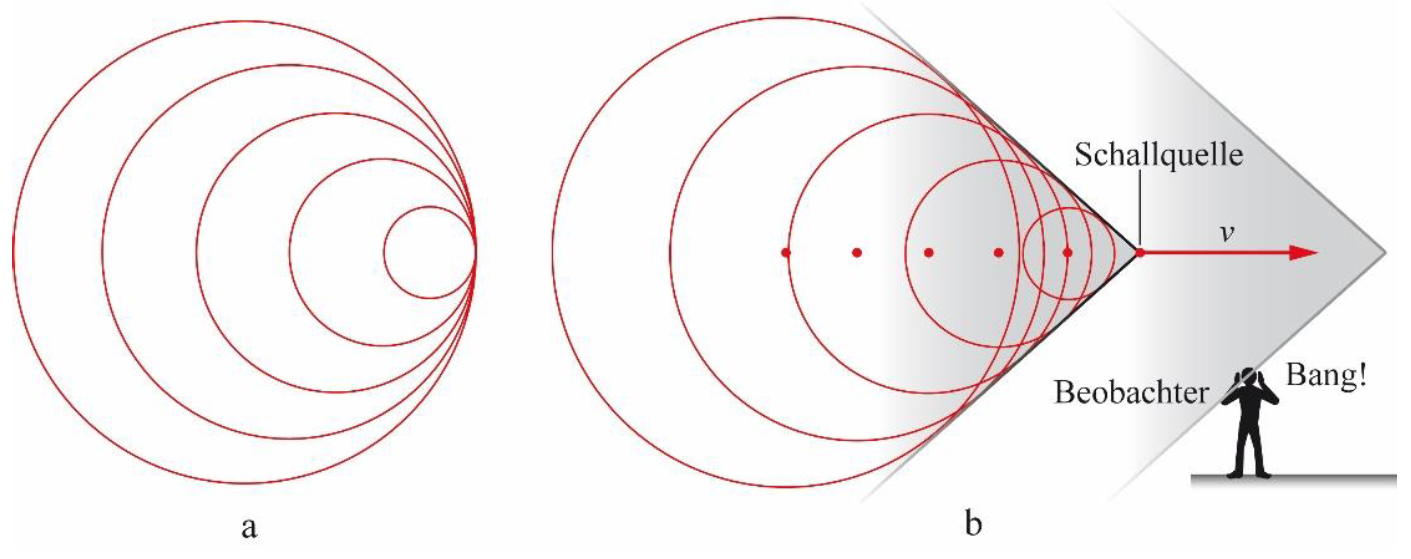
\includegraphics[height=2.2cm, align=t]{images/machkegel_1.png} 
    $$ \boxed{ \sin(\vartheta) = \frac{u \, \Delta t}{v \, \Delta t} = \frac{u}{v} } $$
\end{minipage}
\hfill
\begin{minipage}[t]{0.38\columnwidth}
    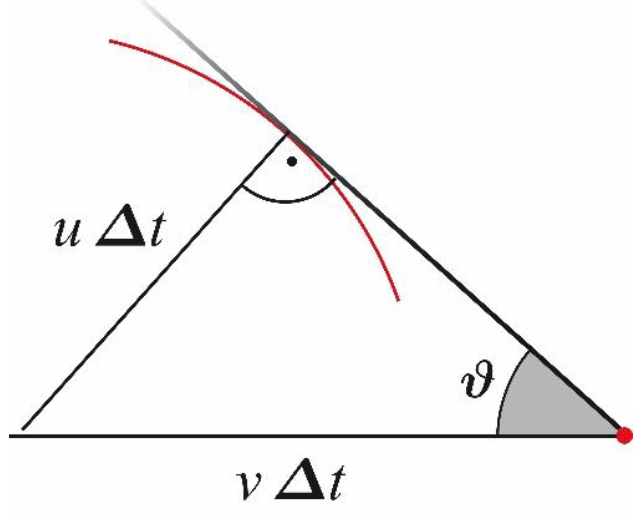
\includegraphics[height=2.2cm, align=t]{images/machkegel_2.png} 
    $$ \boxed{ M = \frac{v}{u} } $$
\end{minipage}


\renewcommand{\arraystretch}{1.1}
\begin{ctabular}{clc}
    $v$ & Geschwindigkeit der Quelle                        & $[v] = \frac{\meter}{\second}$    \\
    $u$ & Wellengeschwindigkeit (Schallgeschwindingkeit)    & $[u] = \frac{\meter}{\second}$    \\
    $M$ & Machzahl                                          & $[M] = 1$
\end{ctabular}
\renewcommand{\arraystretch}{1}


\subsection{Wellenwiderstand, Energietransport -- Schallwellen}

\subsubsection{Terminologie Wellenwiderstand}
Der \textbf{Wellenwiderstand $Z$} (auch \textbf{Impedanz} genannt) beschreibt, wie ein Medium den Fluss von Energie beeinflusst.

\smallskip

\textrightarrow\ \textquotesingle Wie gut können sich Wellen in einem Medium ausbreiten?\textquotesingle

$$ \boxed{ Z = \rho \cdot u = \frac{\Delta p_0}{v_0} } $$


\renewcommand{\arraystretch}{1.4}
\begin{ctabular}{clc}
    $Z$             & Wellenwiderstand bzw. Impedanz    & $[Z] = \ohm = \frac{\pascal}{\meter\per\second} = \frac{\newton \, \second}{\meter\cubed}$    \\
    $\rho$          & Dichte des Mediums                & $[\rho] = \frac{\kilogram}{\meter\cubed}$                                                     \\
    $u$             & Wellengeschwindigkeit             & $[u] = \frac{\meter}{\second}$                                                                \\
    $\Delta p_0$    & Druckamplitude                    & $[\Delta p_0] = \pascal$                                                                      \\
    $v_0$           & Schnellenamplitude                & $[v_0] = \frac{\meter}{\second}$
\end{ctabular}
\renewcommand{\arraystretch}{1}


\subsubsection{Weitere Terminologien}

\renewcommand{\arraystretch}{1.2}
\begin{tabular}{lll}
    Schalldruck                 & $p = \Delta p_0 \, \cos(\omega \, t - k \, x)$    & $[p] = \pascal$                   \\
    Druckamplitude              & $  \Delta p_0 = \rho \, u \, v_0 $                &                                   \\
    \\
    Schallschnelle (Schnelle)   & $v = v_0 \,  \cos(\omega \, t - k \, x)$          & $[v] = \frac{\meter}{\second}$    \\
    Schnellenamplitude          & $v_0 = \omega \, \xi_0$ 
\end{tabular}
\renewcommand{\arraystretch}{1}


\subsubsection{Intensität der Schallwelle}

\textbf{Intensität = gemittelte Energieflussdichte}

\begin{minipage}{0.48\columnwidth}
    $$ E_{\rm kin} = \frac{\rho \cdot v^2}{4} = \frac{\rho \cdot v_0^2}{4} $$
\end{minipage}
\hfill
\begin{minipage}{0.48\columnwidth}
    $$ E_{\rm pot} = \frac{p^2 - p_0^2}{2 \, \rho \, u^2} = \frac{\rho \cdot v_0^2}{4} $$
\end{minipage}

$$ E_{\rm tot} = E_{\rm kin} + E_{\rm pot} = \frac{\rho \cdot v_0^2}{2} $$

$$ \boxed{ I = u \cdot \overline{w} = \frac{1}{2} \rho \, v_0^2 \, u  =  \frac{1}{2} \rho \, (\omega \, \xi_0)^2  \, u = \frac{( \Delta p_0)^2}{2 \, Z} = \frac{P}{A} } $$


\renewcommand{\arraystretch}{1.2}
\begin{ctabular}{clc}
    $I$             &  Schallintensität                                 & $[I] = \frac{\watt}{\meter\squared}$                                                          \\
    $\overline{w}$  & Energieflussdichte                                & $[\overline{w}] = \frac{\watt \, \second}{\meter\cubed}$                                      \\
                    & Pot. Energie \textrightarrow\ 'Kompression Gas'   &                                                                                               \\
                    & Kin. Energie \textrightarrow\ 'Geschw. Teilchen'  &                                                                                               \\
    $\rho$          & Dichte                                            & $[\rho] = \frac{\kilogram}{\meter\cubed}$                                                     \\
    $v_0$ &         Schnellenamplitude                                  & $[v_0] = \frac{\meter}{\second}$                                                              \\
    $\xi_0$         & Amplitude                                         & $[\xi_0]$                                                                                     \\
    $u$             & Wellengeschwindigkeit                             & $[u] = \frac{\meter}{\second}$                                                                \\
    $\Delta p_0$    & Druckamplitude                                    & $[\Delta p_0] = \pascal$                                                                      \\
    $Z$             & Wellenwiderstand bzw. Impedanz                    & $[Z] = \ohm = \frac{\pascal}{\meter\per\second} = \frac{\newton \, \second}{\meter\cubed}$    \\
    $P$             & Leistung                                          & $[P] = \watt$                                                                                 \\
    $A$             & (Abstrahl-) Fläche                                & $[A] = \meter\squared$ 
\end{ctabular}
\renewcommand{\arraystretch}{1}


\subsection{Dispersion}
Die \textbf{Abhängigkeit} der Wellengeschwindigkeit \textbf{von der Wellenlänge} wird als Dispersion bezeichnet.

\smallskip

\textrightarrow\  Siehe Beispiel Optik Abschnitt~\ref{Dispersion Optik}


\subsubsection{Dispersion bei Wasserwellen}

$$ \boxed{ u(\lambda) = \sqrt{\left( \frac{g \cdot \lambda}{2 \, \pi} + \frac{2 \, \pi \cdot \sigma}{\rho \cdot \lambda} \right) \cdot \tanh \left( \frac{2 \, \pi \cdot h}{\lambda} \right) }  } $$


\begin{minipage}{0.48\columnwidth}
    \begin{center}
        Tiefes Wasser ($\lambda \ll h$)
    \end{center}
    $$ \boxed{ u(\lambda) = \sqrt{\frac{g \cdot \lambda}{2 \, \pi}} } $$
\end{minipage}
\hfill
\begin{minipage}{0.48\columnwidth}
    \begin{center}
        Flaches Wasser ($\lambda \gg h$)
    \end{center}
    $$ \boxed{ u = \sqrt{ g \cdot h } } $$
\end{minipage}


\renewcommand{\arraystretch}{1.2}
\begin{ctabular}{clc}
    $g$         & Erdbeschleinigung $g = 9.81 \, \frac{\meter}{\second\squared}$    & $[g] = \frac{\meter}{\second\squared}$    \\
    $\lambda$   & Wellenlänge                                                       & $[\lambda] = \meter $                     \\
    $\sigma$    & Oberflächenspannung                                               & $[\sigma] = \frac{\newton}{\meter}$       \\
    $h$         & Wassertiefe                                                       & $[h] = \meter$                            \\
    $\rho$      & Dichte                                                            & $[\rho] = \frac{\kilogram}{\meter\cubed}$
\end{ctabular}
\renewcommand{\arraystretch}{1}


        \section{Superposition von Wellen}

\textbf{Superposition beschreibt die Überlagerung (Addition) von Wellen}

\smallskip

\begin{itemize}
	\item Linearität der Wellengleichung 
	\item Die Summe zweier Lösungen der Wellengleichung ist auch eine  der Wellengleichung.
\end{itemize}

\smallskip

Das Superpositionsprinzip erlaubt die Darstellung von periodischen Wellen als eine Summe von harmonischen Wellen.


\subsection{Schwebung}

Superposition von Wellen mit \textbf{unterschiedlichen} Frequenzen \textrightarrow\  Hörbar als ein \textquotesingle Flattern\textquotesingle

$$ \boxed{f_{\text{Schwebung}} = f_2 - f_1 } $$

\begin{minipage}{0.48\columnwidth}
    $$ \xi_1 = A \cdot \sin(\omega_1 \, t) $$
\end{minipage}
\hfill
\begin{minipage}{0.48\columnwidth}
    $$ \xi_2 = A \cdot \sin(\omega_2 \, t) $$
\end{minipage}

\[
    \boxed{ \xi = 2 \, A \cdot \sin( \overline{\omega} \, t) \cdot \cos( \Omega \, t) } \qquad
    \text{mit } \overline{\omega} = \frac{\omega_1 + \omega_2}{2} \quad \text{und} \quad \Omega = \frac{\omega_2 - \omega_1}{2}
\]


\subsection{Interferenz}

Superposition von Wellen mit \textbf{gleichen} Frequenzen

\begin{minipage}[t]{0.35\columnwidth}
    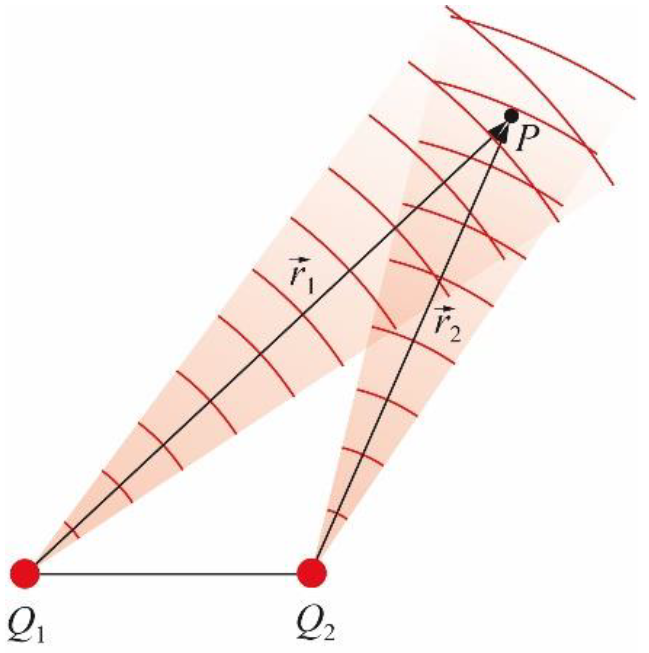
\includegraphics[width=\columnwidth, align=t]{images/interferenz.png}
\end{minipage}
\hfill
\begin{minipage}[t]{0.63\columnwidth}
    $$ \xi_1 = A \cdot \sin(\omega \, t - k \, r_1) $$
    $$ \xi_2 = A \cdot \sin(\omega \, t - k \, r_2) $$
    $$ \boxed{ \xi = 2 \, A \cdot \sin \left( \omega \, t - \frac{k (r_1 + r_2)}{2} \right) \,  \cos \left( \frac{k(r_2 - r_1)}{2}  \right) } $$

    \textrightarrow\  Der $\cos$-Term hängt nur vom Ort ab! \\
    \textrightarrow\  Es gibt \textbf{Orte}, an denen Welle sich auslöscht!
\end{minipage}



\subsection{Kohärenz}

Zwei Wellen werden als kohärent bezeichnet, wenn eine \textbf{feste Phasendifferenz} zwischen den beiden Wellen besteht.

\smallskip

\begin{outline}
    \1 Kohärenz ist eine \textbf{Vorbedingung}, damit sich eine \textbf{Interferenz} bilden kann
    \1 \textbf{Kohärenzlänge} ist der \textbf{maximale Streckenunterschied}, den zwei Wellen haben dürfen, damit eine \textbf{(stabile) Interferenz} beobachtet werden kann.
\end{outline}


\subsection{Reflexion und Transmission}

\subsubsection{Verhalten von Wellem an Grenzflächen von zwei Medien}

Ein Teil der Welle wird reflektiert und ein Teil wird transmittiert

\smallskip

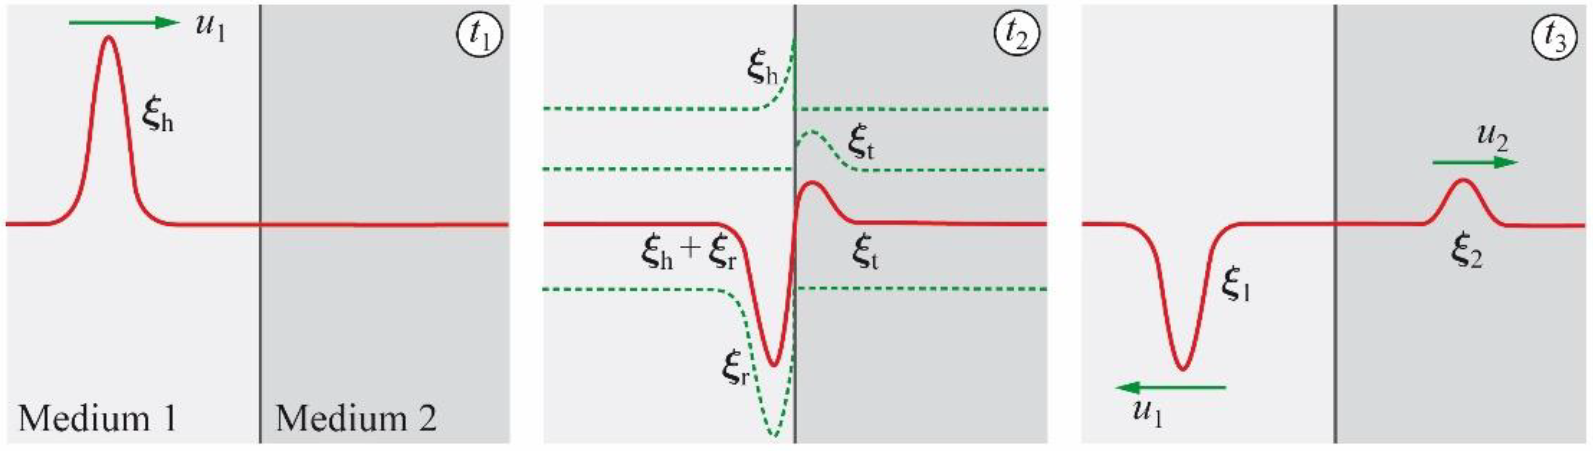
\includegraphics[width=\columnwidth]{images/reflexion_transmission.png}

\medskip
\paragraph{Physikalische Bedingung}

Stetigkeit der Wellenfunktion und der Ableitung an der Grenzfläche

$$ \xi_1(0) = \xi_2(0) \qquad \qquad \dot{\xi}_1(0) = \dot{\xi}_2(0) $$


\subsubsection{Intensität von Reflexion und Transmission}\label{Reflexion}

\begin{minipage}[t]{0.4\columnwidth}
    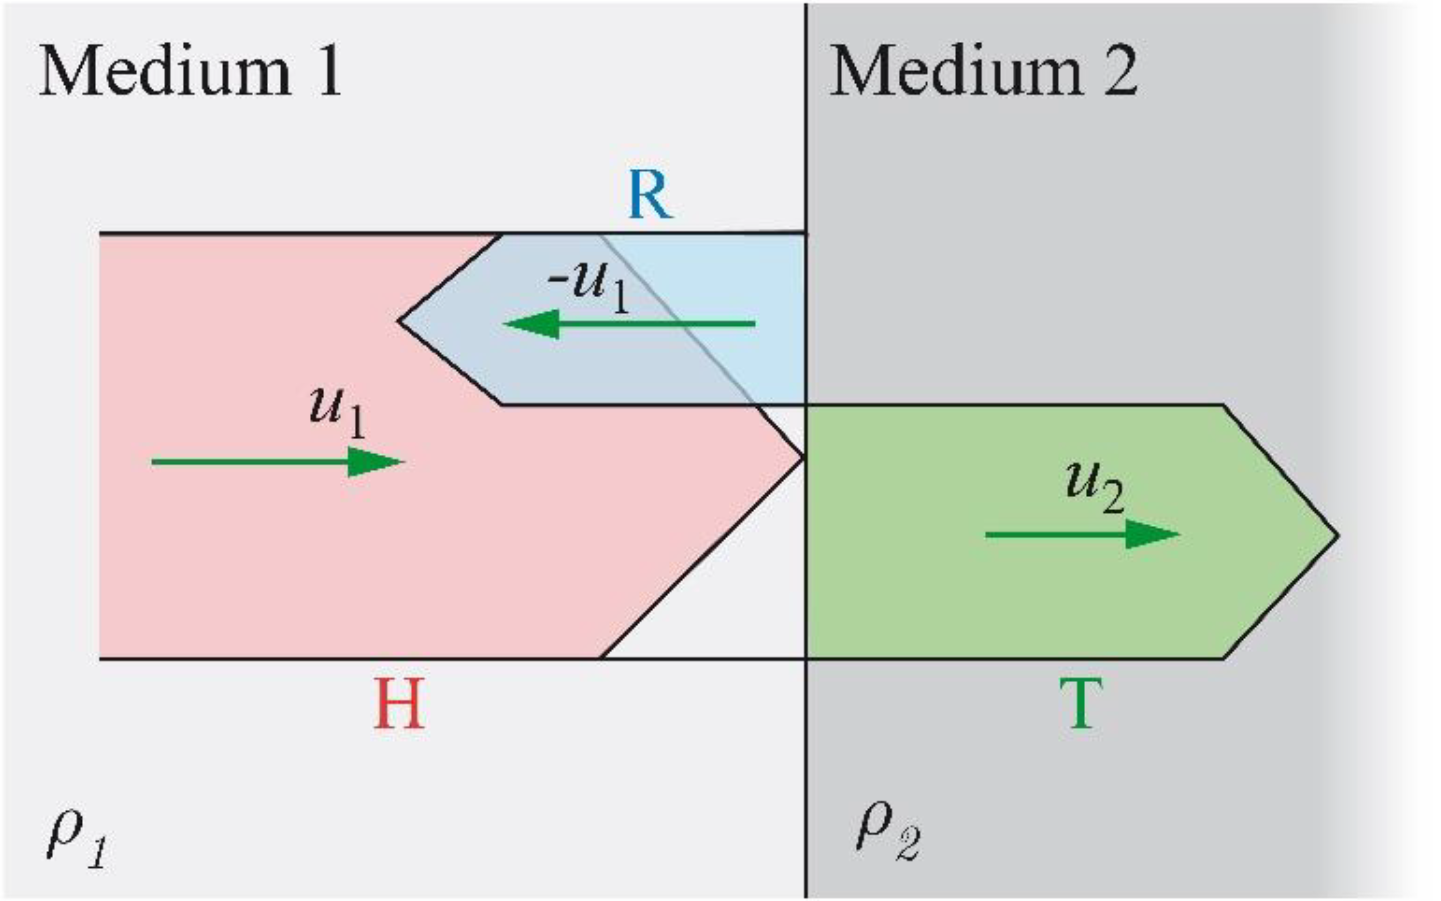
\includegraphics[width=\columnwidth, align=t]{images/reflexionskoeffizient_transmissionskoeffizient.png}
\end{minipage}
\hfill
\begin{minipage}[t]{0.58\columnwidth}
    \[ 
        \boxed{ R = \left(  \frac{Z_1 - Z_2}{Z_1 + Z_2}  \right)^2  } \qquad
        \boxed{ T = \frac{ 4 \cdot Z_1 \cdot Z_2}{(Z_1 + Z_2)^2}   }
    \]
    $$ \boxed{ \sqrt{R} = \frac{Z_1 - Z_2}{Z_1 + Z_2} = \frac{u_R}{u_H}  =\frac{A_R}{A_H} = \frac{p_R}{p_H} = \ldots } $$
    $$ \boxed{ \frac{2 \cdot Z_2}{Z_1 + Z_2} = \frac{u_T}{u_H} = \frac{A_T}{A_H} = \frac{p_T}{p_H} = \ldots } $$
\end{minipage}

\renewcommand{\arraystretch}{1.1}
\begin{ctabular}{clc}
    $R$     & Reflexionskoeffizient                 & $[R] = 1$                                                                                     \\
    $T$     & Transmissionskoeffizient              & $[T] = 1 $                                                                                    \\
    $u_H$   & Geschwindigkeit hinlaufende Welle     & $[u_H] = \frac{\meter}{\second}$                                                              \\
    $u_R$   & Geschwindigkeit reflektierte Welle    & $[u_R] = \frac{\meter}{\second}$                                                              \\
    $u_T$   & Geschwindigkeit transmittierte Welle  & $[u_T] = \frac{\meter}{\second}$                                                              \\
    $p_H$   & Druck hinlaufende Welle               & $[p_H] = \pascal$                                                                             \\
    $p_R$   & Druck reflektiert Welle               & $[p_R] = \pascal$                                                                             \\
    $p_T$   & Druck transmittierte Welle            & $[p_T] = \pascal$                                                                             \\
    $A_H$   & Amplitude hinlaufende Welle           & $[A_H] = 1$                                                                                   \\
    $A_R$   & Amplitude reflektiert Wellen          & $[A_R] = 1$                                                                                   \\
    $A_T$   & Amplitude transmittierte Welle        & $[A_T] = 1$                                                                                   \\
    $Z_i$   & Wellenwiderstand im Medium $i$        & $[Z] = \ohm = \frac{\pascal}{\meter\per\second} = \frac{\newton \, \second}{\meter\cubed}$
\end{ctabular}
\renewcommand{\arraystretch}{1}


\subsubsection{Phasensprünge bei Reflexionen}

\begin{minipage}{0.4\columnwidth}
    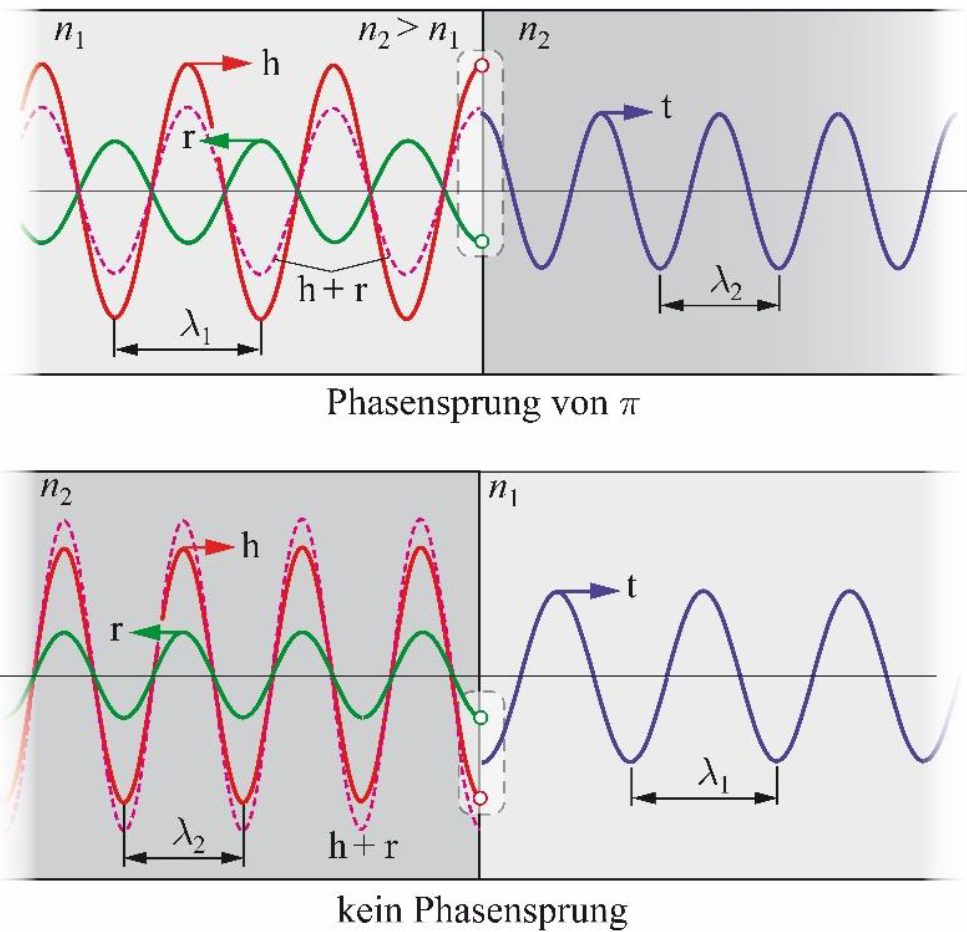
\includegraphics[width=0.9\columnwidth]{images/reflexion_phasensprung.png}
\end{minipage}
\hfill
\begin{minipage}{0.58\columnwidth}
    Reflexion an 'dichtem' Material \\
    \textrightarrow\  \textbf{Phasensprung}

    \medskip
    dicht: $n_2 > n_1$ \\
    \textbf{kleinere} Wellengeschwindigkeit, \textbf{grösserer} Wellenwiderstand

    \medskip
    Reflexion an 'dünnem' Material\\
    \textrightarrow\  \textbf{kein Phasensprung}
\end{minipage}


\subsection{Anwendung: Elektromagnetische Wellen}

\subsubsection{Elektromagnetische Wellem in Doppelleiter}

\begin{minipage}{0.48\columnwidth}
    $$ \boxed{ U_r = \frac{Z_2 - Z_1}{Z_1 + Z_2} \, U_h } $$
\end{minipage}
\hfill
\begin{minipage}{0.48\columnwidth}
    $$ \boxed{ U_t = \frac{2 \, Z_2}{Z_1 + Z_2} \, U_h } $$
\end{minipage}

\begin{minipage}{0.48\columnwidth}
    $$ \boxed{ I_r = \frac{Z_2 - Z_1}{Z_1 + Z_2} \, I_h } $$
\end{minipage}
\hfill
\begin{minipage}{0.48\columnwidth}
    $$ \boxed{ I_t = \frac{2 \, Z_1}{Z_1 + Z_2} \, I_h } $$
\end{minipage}

\medskip


\paragraph{Kabel mit kurzgeschlossenem Ende $\boldsymbol{Z_2 = 0}$}

\begin{minipage}{0.3\columnwidth}
    $$ U_r = - U_h $$
\end{minipage}
\hfill
\begin{minipage}{0.68\columnwidth}
    $$ U_1 = U_h + U_r  = U_h - U_h = 0 $$
\end{minipage}

\medskip


\paragraph{Kabel mit offenem Ende $\boldsymbol{Z_2 = \infty}$}

\begin{minipage}{0.3\columnwidth}
    $$ I_r = - I_h $$ 
\end{minipage}
\hfill
\begin{minipage}{0.68\columnwidth}
    $$ I_1 = I_r + I_h  = I_r - I_r = 0 $$  
\end{minipage}


\renewcommand{\arraystretch}{1.1}
\begin{ctabular}{clc}
    $U_r$ & Reflektierte Spannung               & $[U_r] = \volt$                                                                               \\
    $U_h$ & Eintreffende Spannung               & $[U_h] = \volt$                                                                               \\
    $I_r$ & Reflektierter Strom                 & $[I_r] = \ampere$                                                                             \\
    $I_h$ & Eintreffender Strom                 & $[I_h] = \ampere$                                                                             \\
    $Z_i$ & Wellenwiderstand im Medium $i$      & $[Z] = \ohm = \frac{\pascal}{\meter\per\second} = \frac{\newton \, \second}{\meter\cubed}$
\end{ctabular}
\renewcommand{\arraystretch}{1}


\subsubsection{Elektromagnetische Wellen in homogenem Milieu}

\[
    \boxed{ Z = \frac{E}{H} = \sqrt{ \frac{\mu_r \mu_0}{\varepsilon_r \varepsilon_0}} = \sqrt{\frac{\mu_r}{\varepsilon_r}} Z_0 = Z_0 \frac{c}{n}} \qquad 
    \boxed{ R = \left(  \frac{Z_1 - Z_2}{Z_1 + Z_2}  \right)^2 =  \left(  \frac{n_1 - n_2}{n_1 + n_2}  \right)^2 }
\]



\renewcommand{\arraystretch}{1.1}
\begin{ctabular}{clc}
    $R$             & Reflexionskoeffizient             & $[R] = 1$                                                                                     \\
    $Z_i$           & Wellenwiderstand im Medium $i$    & $[Z] = \ohm = \frac{\pascal}{\meter\per\second} = \frac{\newton \, \second}{\meter\cubed}$    \\
    $\mu_r$         & Permeabilitätszahl                & $[\mu_r] = 1$                                                                                 \\
    $\varepsilon$   & Dielektizitätszahl                & $[\varepsilon_r] = 1$                                                                         \\
    $n_i$           & Brechungsindex von Medium $i$     & $[n_1] = 1$
\end{ctabular}

\renewcommand{\arraystretch}{1.2}
\begin{ctabular}{lll}
    $\varepsilon_0$ & Ele. Feldkonstante        & $\varepsilon_0 = 8.854 \cdot 10^{-12} \, \frac{\ampere \, \second}{\volt \, \meter}$  \\
    $\mu_0$         & Magn. Feldkonstante       & $\mu_0 = 4 \pi \cdot 10^{-7} \frac{\newton}{\ampere\squared}$                         \\
    $Z_0$           & Wellenwiderstand Vakuum   & $Z_0 \approx 376.73 \, \ohm$                                                          \\
    $c$             & Lichtgeschwindigkeit      & $c = 300 \cdot 10^6 \, \frac{\meter}{\second}$
\end{ctabular}
\renewcommand{\arraystretch}{1}

\columnbreak


        \section{Stehende Wellen}

\subsection{Terminologie}

Eine \textbf{stehende Welle} ist eine Welle, bei der Orte maximaler Auslenkung (oder minimaler Auslenkungen) sich \textbf{nicht fortbewegen}. 

\smallskip

\begin{itemize}
	\item Ort- und Zeitabhängigkeit sind separiert 
	\item Die Welle bewegt sich nicht im Raum ('Muster bleibt stehen') 
\end{itemize}

$$ \boxed{ \xi(x, t) = \xi_0 \cdot \cos(\omega t) \cdot \cos(k x) }  \qquad \quad \text{ \textrightarrow\ } \sin() \text{-Terme sind auch erlaubt!} $$

\medskip

\begin{outline}
    \1 Orte, wo die Welle für alle Zeit $= 0$ ist heissen \textbf{Wellenknoten} \\
        \textrightarrow\ \textbf{Zwei benachbarte Knoten sind $\boldsymbol{\frac{\lambda}{2}}$ auseinander}
    \1 Orte, wo die Welle eine maximale Auslenkung erreicht, heissen \textbf{Wellenbauch} \\
        \textrightarrow\ \textbf{Zwei benachbarte Bäuche sind $\boldsymbol{\frac{\lambda}{2}}$ auseinander}
\end{outline}



\subsection{Entstehung von stehenden Wellen}

\begin{center}
    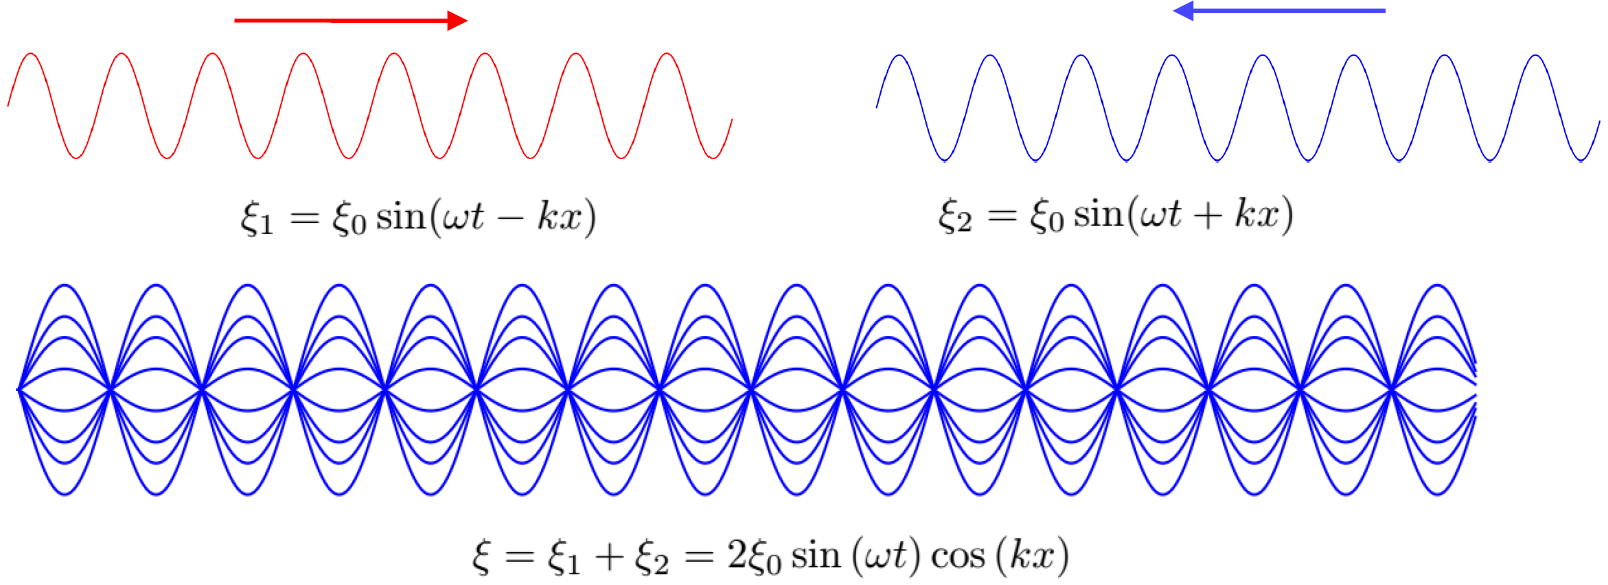
\includegraphics[width=0.85\columnwidth]{images/stehende_wellen.png}
\end{center}



\subsection{Prinzip von Huygens}

\begin{minipage}[t]{0.4\columnwidth}
    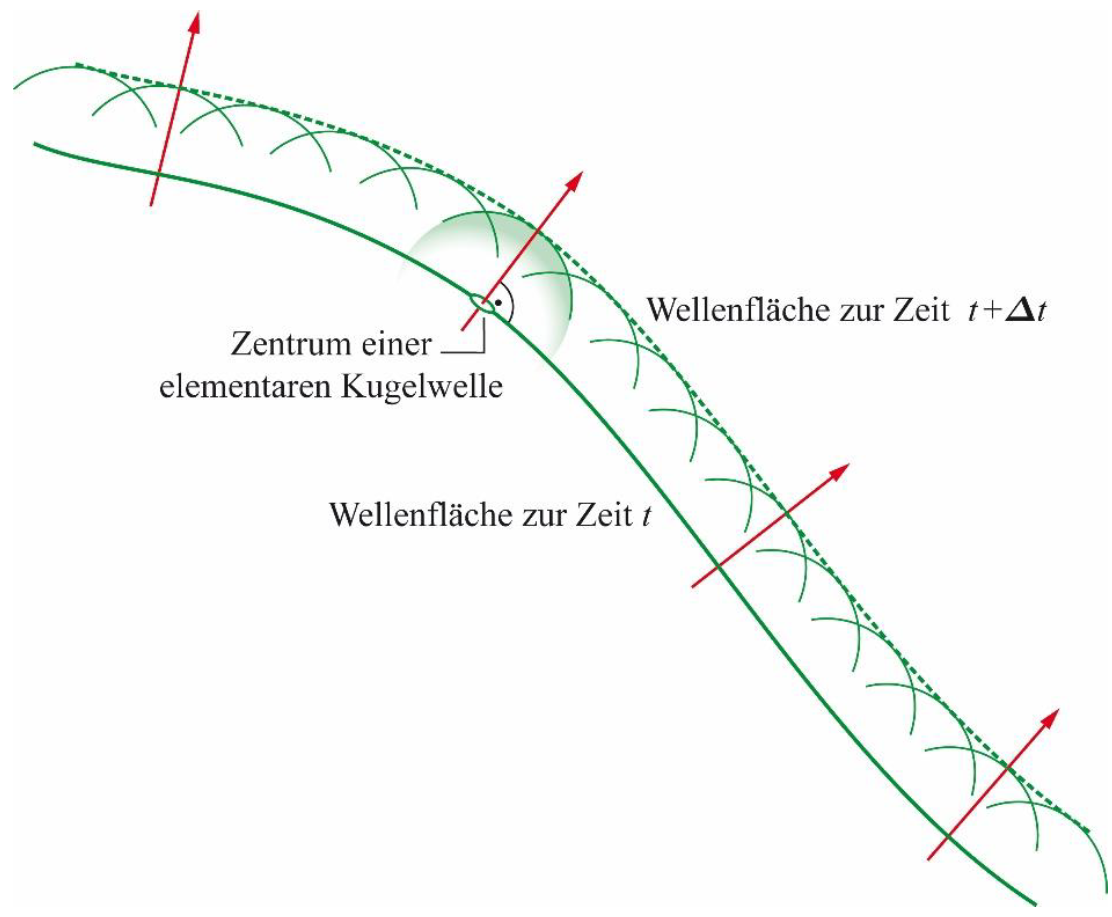
\includegraphics[width=\columnwidth, align=t]{images/huygens.png}
\end{minipage}
\hfill
\begin{minipage}[t]{0.55\columnwidth}
    \raggedright
    Jedes Flächenelement auf einer Wellenfläche kann als Zentrum einer Kugelwelle betrachtet werden. \\
    Die Wellenfläche zu einem späteren Zeitpunkt ist die Einhüllende all dieser Elementarwellen.
\end{minipage}


\subsection{Eigenschwingungen -- 1D}

\begin{minipage}{0.3\columnwidth}
    $$ \boxed{ f_n = \frac{n}{2 \, l} \cdot u = \frac{u}{\lambda_n} } $$
\end{minipage}
\hfill
\begin{minipage}{0.66\columnwidth}
    $$ \boxed{ \text{Auslenkung = 0: }\quad k_n \cdot l = n \cdot \pi } $$
    $$ \boxed{ \text{Auslenkung max: }\quad k_n \cdot l = \frac{\pi}{2} + n \cdot \pi } $$
\end{minipage}


\subsubsection{Saite}

\begin{itemize}
	\item Reflexion an einer Grenzfläche $\rightarrow$  Stehende Welle 
	\item Stehende Welle muss in vorhandenen Raum passen \textrightarrow\ Geometrische Bedingung 
	\item \textbf{Knoten an beiden Enden} 
\end{itemize}

\smallskip

\begin{minipage}{0.48\columnwidth}
    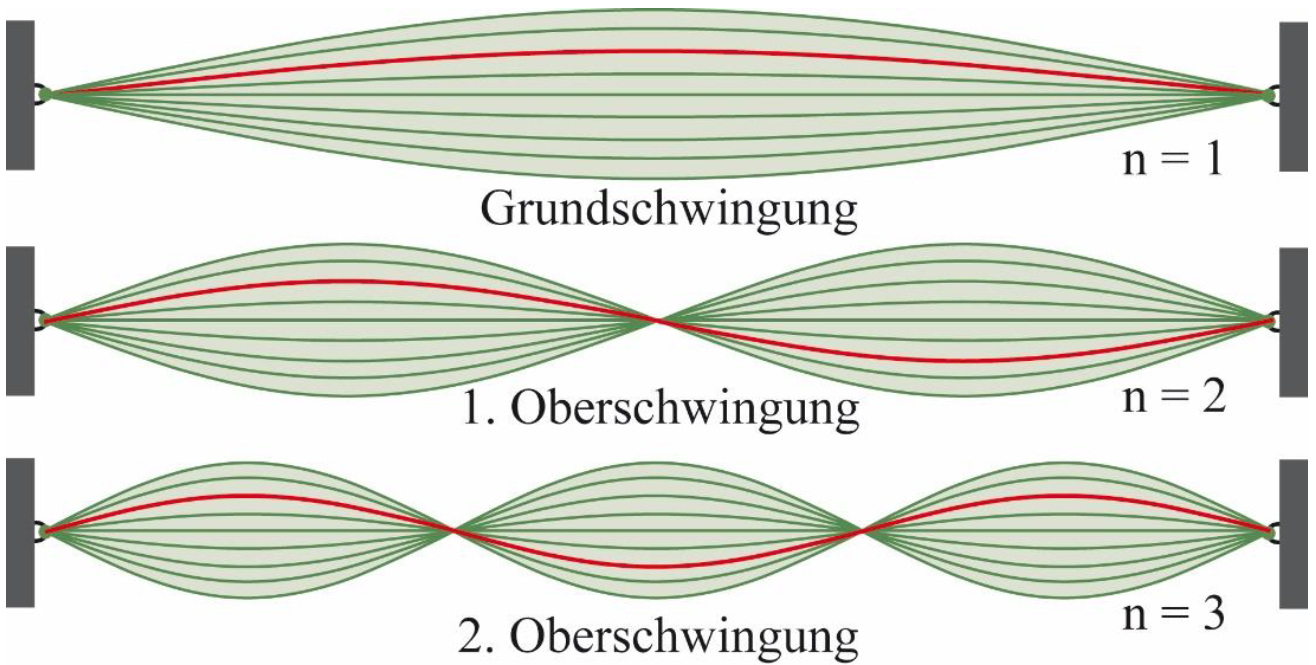
\includegraphics[width=\columnwidth]{images/saite.png}
\end{minipage}
\hfill
\begin{minipage}{0.48\columnwidth}
    $$ \boxed{ \xi = \xi_0 \, \sin(\omega t) \cdot \sin(k x)  } $$
    $$ \boxed{ \text{Auslenkung = 0: } k_n \cdot l = n \cdot \pi } $$
    $$ \boxed{ f_n = \frac{u}{\lambda_n} = \frac{n}{2 \, l} \cdot u = \frac{n}{2 \, l} \sqrt{\frac{F}{\rho \cdot A}} } $$
\end{minipage}

\renewcommand{\arraystretch}{1.2}
\begin{ctabular}{clc}
    $k_n$       & Wellenzahl                & $[k_n] = \frac{1}{\meter}$        \\
    $l$         & Länge der Saite           & $[l] = \meter$                    \\
    $u$         & Wellengeschwindigkeit     & $[u] = \frac{\meter}{\second}$    \\
    $\lambda_n$ & Wellenlänge               & $[\lambda_n]= \meter$             \\
    $n$         & Ganze Zahl                & $[n] = 1$                         \\
    $\omega$    & Kreisfrequenz             & $[\omega] = \frac{\rad}{\second}$ \\
    $A$         & Querschnitt der Saite     & $[A] = \meter\squared$
\end{ctabular}
\renewcommand{\arraystretch}{1}


\subsubsection{Pfeiffen}

\begin{minipage}[t]{0.48\columnwidth}
    \paragraph{Offene Pfeiffe}
    Länge $l = \frac{\lambda}{2}$

    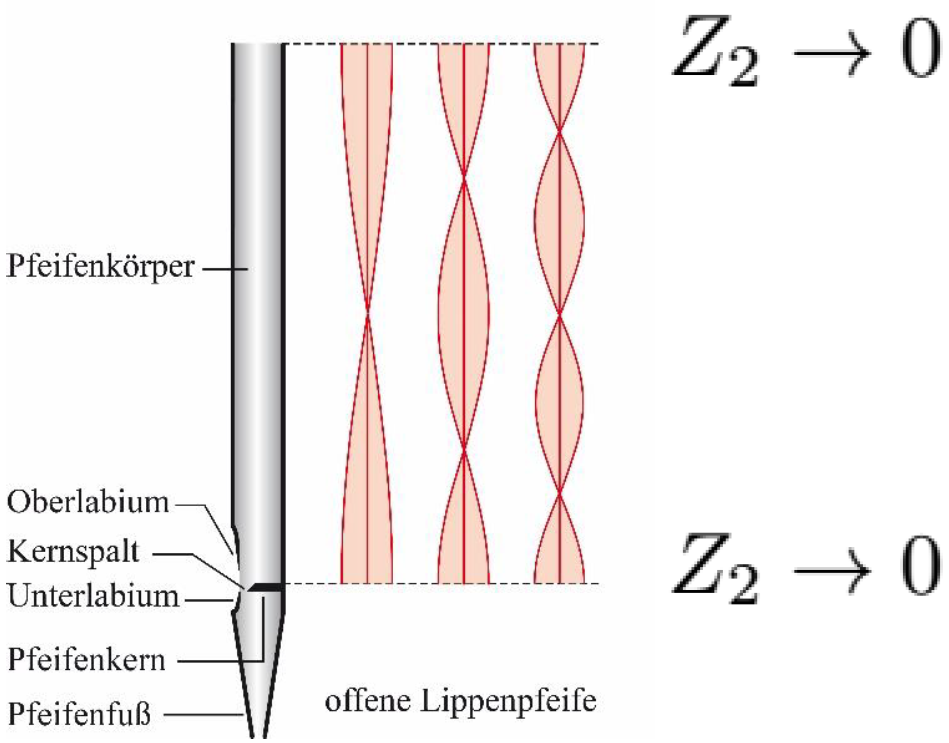
\includegraphics[width=0.85\columnwidth, align=t]{images/offene_pfeiffe.png}

    \smallskip

    Auslenkung an Enden: \\
    Wellenbauch
\end{minipage}
\hfill
\begin{minipage}[t]{0.48\columnwidth}
    \paragraph{Gedackte Pfeiffe}
    Länge $l = \frac{\lambda}{4}$

    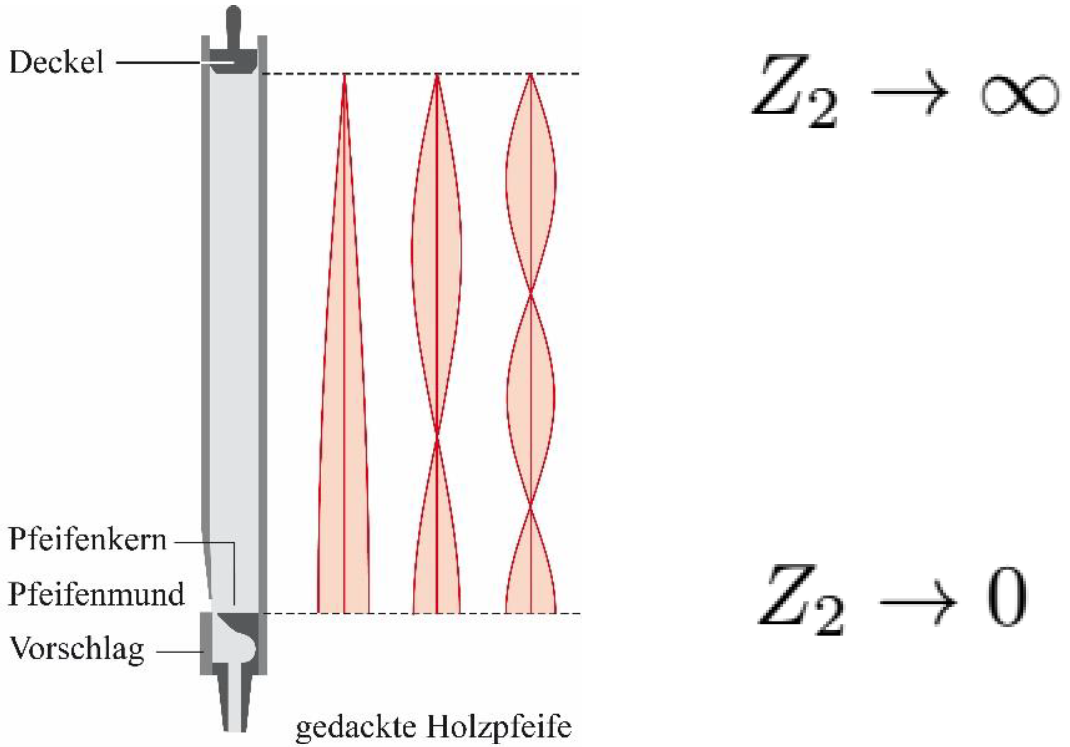
\includegraphics[width=0.9\columnwidth, align=t]{images/gedackte_pfeiffe.png}

    \smallskip

    Auslenkung offenes Ende: \\
    Wellenbauch \\
    Auslenkung gedacktes Ende:\\
    Knoten (max. Auslenkung)
\end{minipage}


\subsection{Eigenschwingungen -- 2D}

\subsubsection{Rechteckige Membrane}

\begin{minipage}{0.3\columnwidth}
    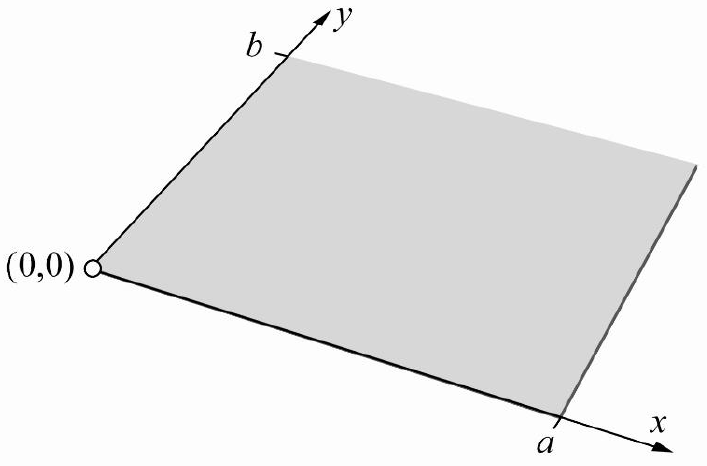
\includegraphics[width=\columnwidth]{images/membrane.png}
\end{minipage}
\hfill
\begin{minipage}{0.68\columnwidth}
    $$ \boxed{ \xi(x,y,t) = \xi_0 \, \sin(\omega t) \, \sin(k_x x) \, \sin(k_y y)  } $$

    $$ \boxed{ \text{Wellenvektor:} \quad  k = |\vec{k}| = \sqrt{k_x^2 + k_y^2}} $$

    $$ \boxed{ u^2 = \frac{\omega^2}{k^2}} $$
\end{minipage}

\medskip

\paragraph{Randbedingungen}

\begin{tabular}{l c c }
    Auslenkung = 0 &  $ \boxed{ k_x = \frac{n \, \pi}{a} }$ & $ \boxed{ k_y = \frac{m \, \pi}{b} }$
\end{tabular} 


        \section{Beugung}

\subsubsection{Terminologie}

Die \textbf{Richtungsänderungen} der Wellenausbreitung in einem homogenen Medium durch \textbf{Hindernisse} wird als \textbf{Beugung (Diffraction)} bezeichnet.

\smallskip

\begin{itemize}
	\item Das Hindernis kann eine Kante, ein Spalt oder ein kleines Objekt sein 
	\item Beugung tritt auf, wenn das \textbf{Hindernis} von \textbf{ähnlicher Grösse} ist, wie die \textbf{Wellenlänge} 
\end{itemize}

\smallskip

\textrightarrow\ \textbf{Beugung tritt auf, wenn eine Welle limitiert wird!}

\medskip

Dies gilt insbesondere für: 
Spalt, Kante, Loch (Pinhole), Objektiv-Öffnung


\subsection{Beugung -- Spalt}

\subsubsection{Beschreibung Setup}\label{Beschreibung Setup}

\begin{center}
    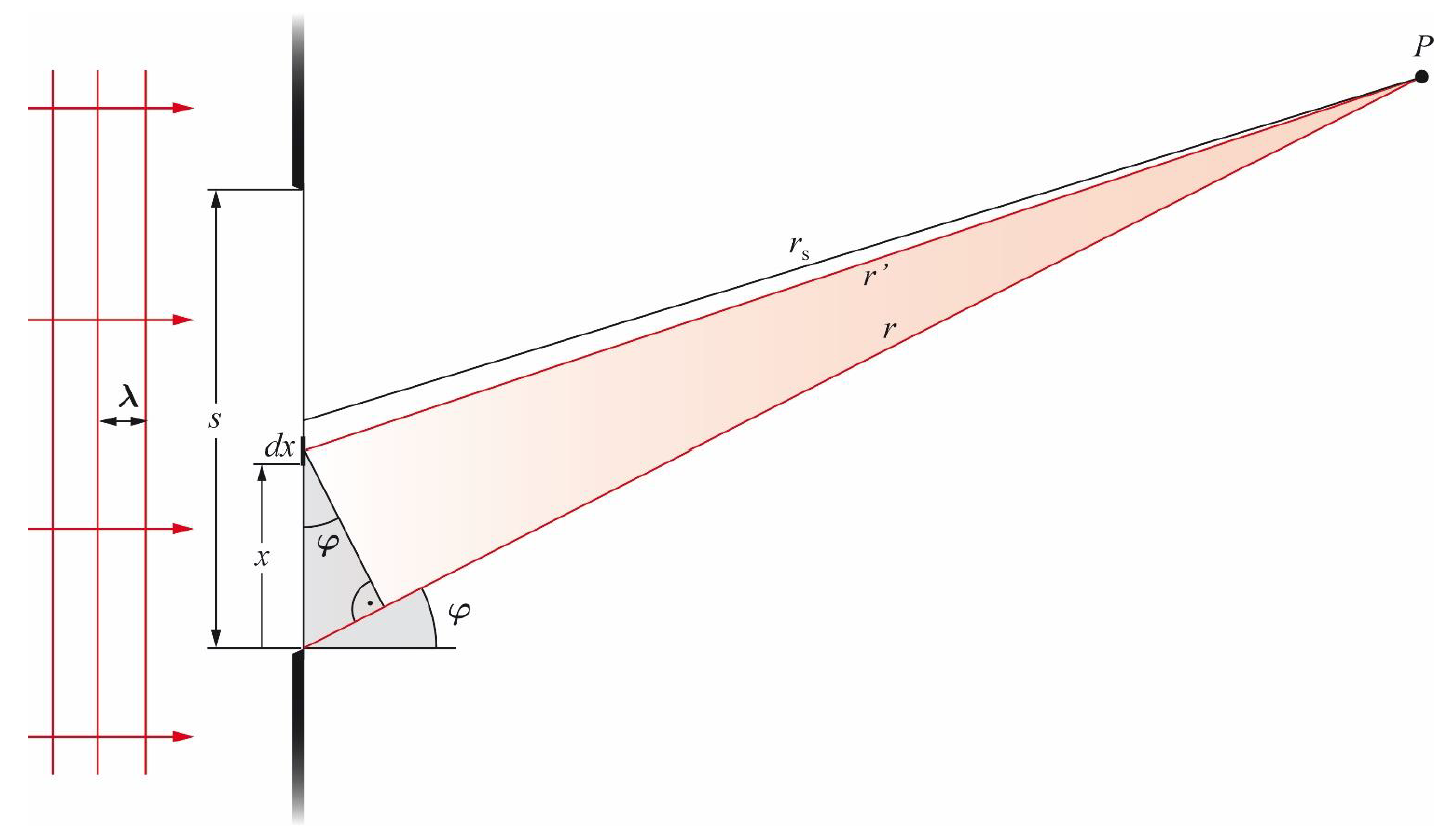
\includegraphics[width=0.7\columnwidth]{images/beugung_spalt.png}
\end{center}


\subsubsection{Intensität nach dem Spalt}

\begin{minipage}[t]{0.58\columnwidth}
    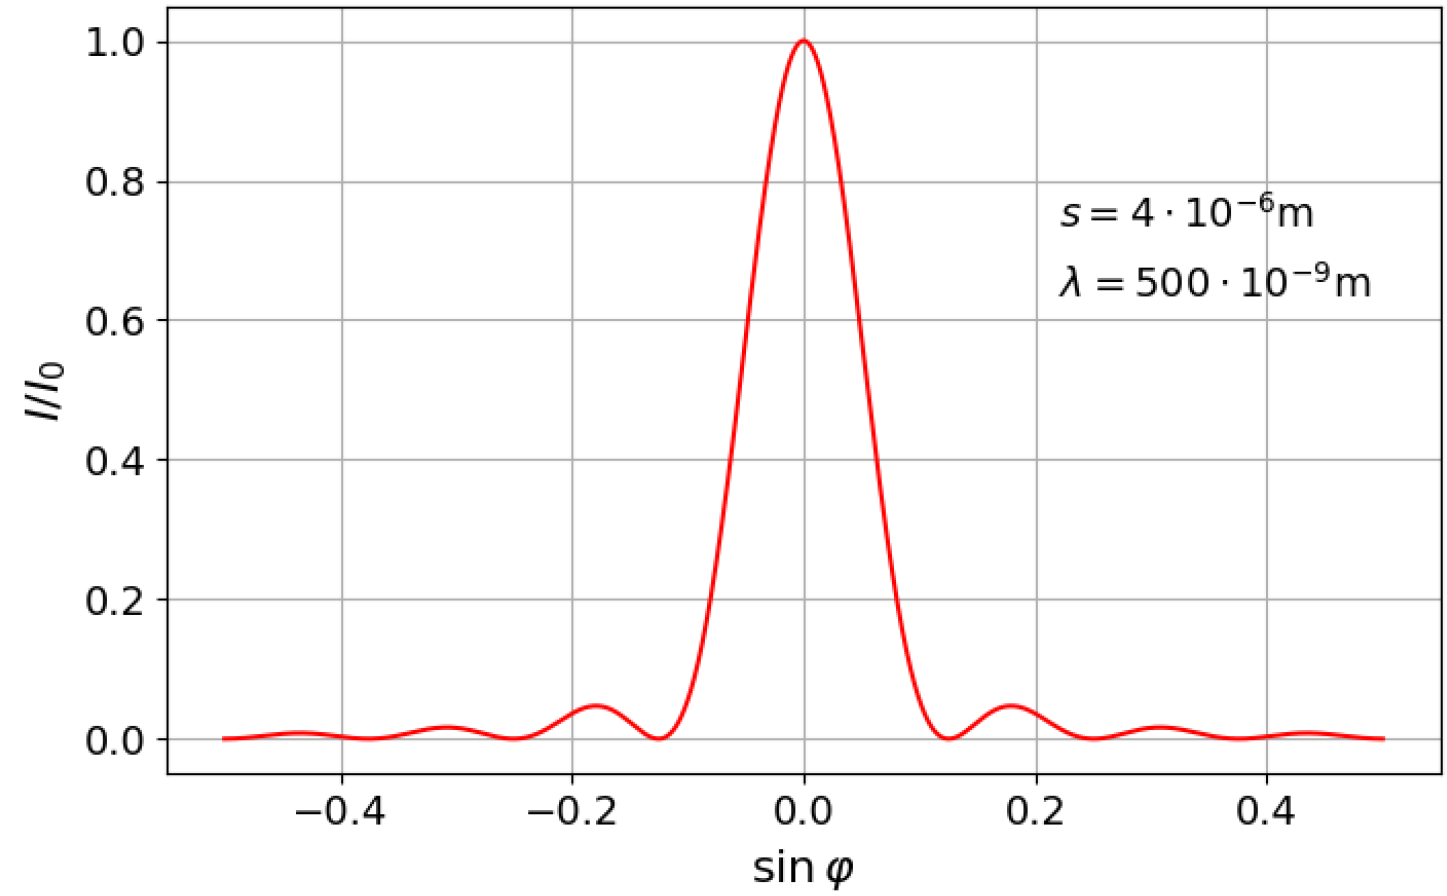
\includegraphics[width=\columnwidth, align=t]{images/beugung_spalt_intensitaet.png}
\end{minipage}
\hfill
\begin{minipage}[t]{0.4\columnwidth}
    $$ \boxed{ I_s \varpropto \frac{A^2}{r^2} \frac{\sin^2\left( \frac{k \cdot s \cdot \sin(\varphi)}{2} \right) }{\left( \frac{k \cdot s \cdot \sin(\varphi)}{2} \right) } } $$

    \smallskip

    \paragraph{Minima der Intensität} 
    $$ \boxed{ \sin(\varphi) = n \, \frac{\lambda}{s}} $$
\end{minipage}

\renewcommand{\arraystretch}{1.2}
\begin{ctabular}{clc}
    $I_s$       & Intensität                                                            & $[I_s] = \frac{W}{\meter\squared}$    \\
    $s$         & Länge des Spalts                                                      & $[s] = \meter$                        \\
    $\lambda$   & Wellenlänge                                                           & $[\lambda]= \meter$                   \\
    $n$         & Ordnung (typ. 1)                                                      & $[n] = 1$                             \\
    $A$         & Amplitude                                                             & $[A]$                                 \\
    $r$         & siehe Bild Abschnitt \ref{Beschreibung Setup}                         & $[r] = \meter$                        \\
    $\varphi$   & Einfallswinkel der Welle zum Spalt                                    & $[\varphi] =$°                        \\
                & \cbl{Hinweis: Oft muss gegebenes $\varphi$ durch 2 geteilt werden!}   &                                       \\
    % & \cbl{geteilt werden!}
\end{ctabular}
\renewcommand{\arraystretch}{1}


\subsection{Beugung -- Runde Öffnung (2D)}

\begin{minipage}[t]{0.48\columnwidth}
    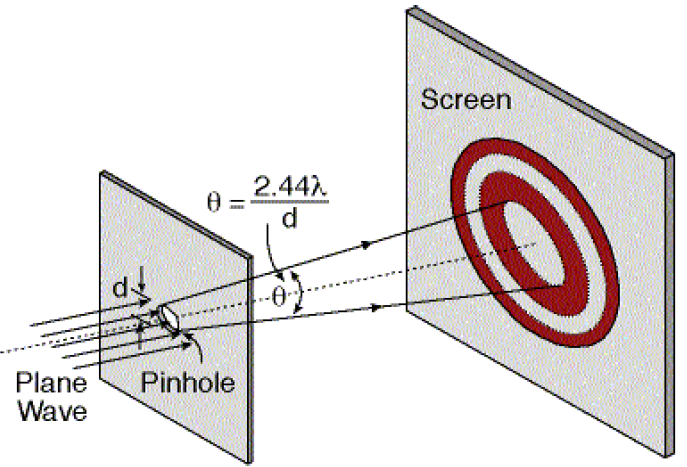
\includegraphics[width=\columnwidth, align=t]{images/beugung_loch.png}
\end{minipage}
\hfill
\begin{minipage}[t]{0.48\columnwidth}
    \paragraph{Nullstelle erster Ordnung} 
    $$ \boxed{ \sin(\varphi) = 1.22 \frac{\lambda}{D} } $$ 

    \renewcommand{\arraystretch}{1.2}
    \begin{ctabular}{clc}
        $\lambda$   & Wellenlänge       & $[\lambda]= \meter$ \\
        $D$         & Loch-Durchmesser  & $[D] = \meter$
    \end{ctabular}
    \renewcommand{\arraystretch}{1}
\end{minipage}


\subsection{Beugung -- Gitter}

\subsubsection{Beschreibung Setup}

\begin{center}
    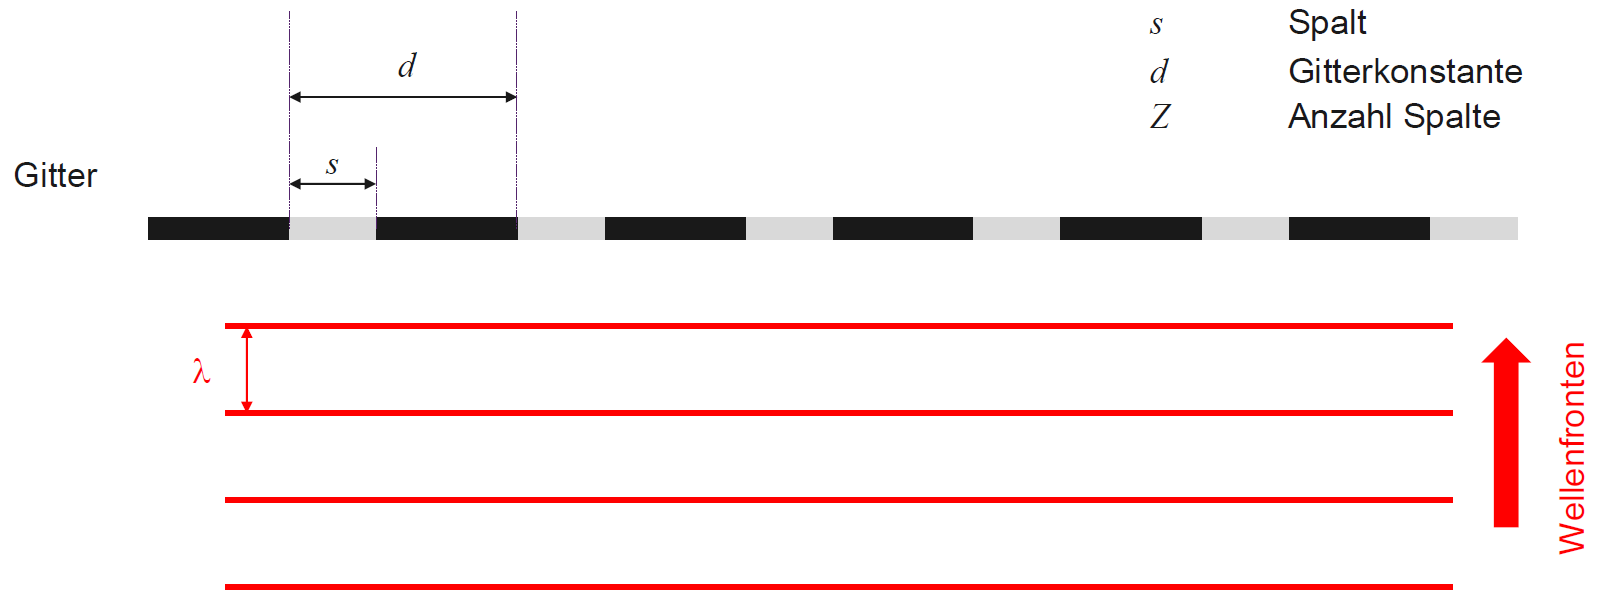
\includegraphics[width=0.85\columnwidth]{images/beugung_gitter.png}
\end{center}


\subsubsection{Intensität nach dem Gitter}

$$ \boxed{ I_G = \frac{A^2}{r^2} \textcolor{red}{A_s^2} \, \textcolor{green}{B^2} } $$

\begin{center}
    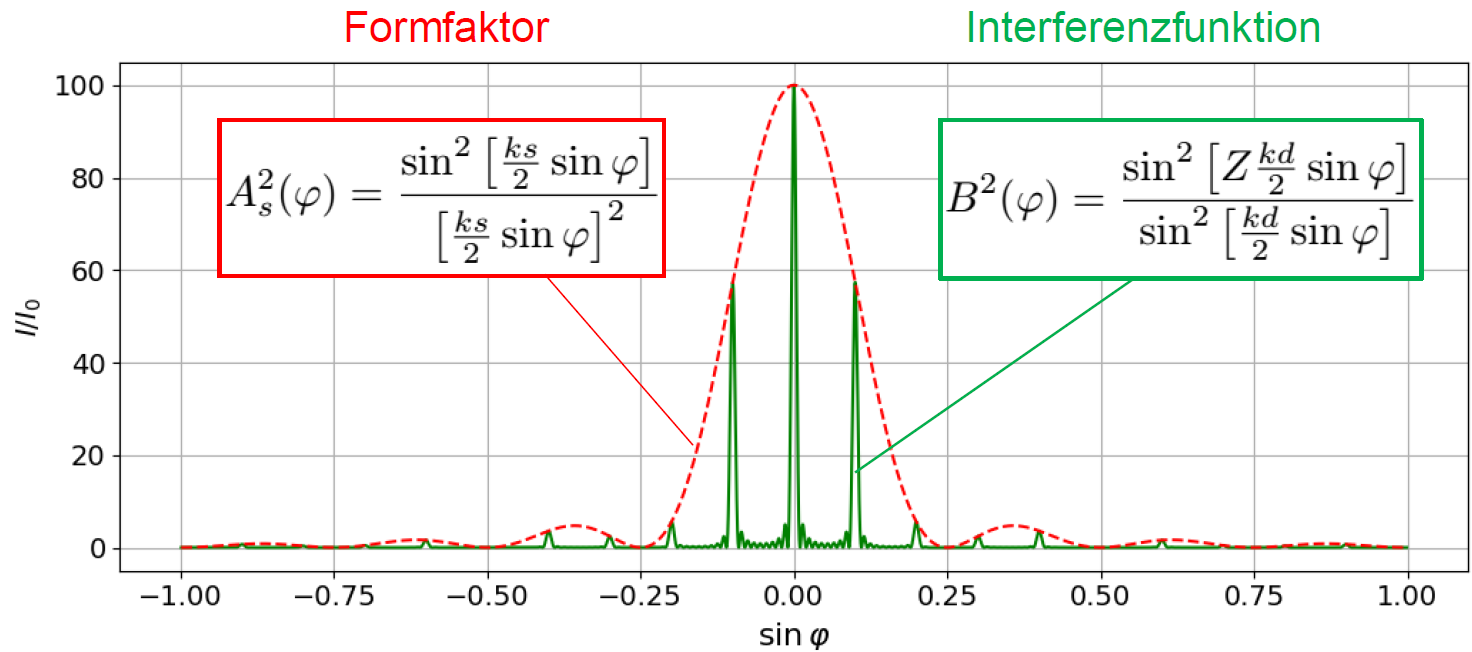
\includegraphics[width=0.9\columnwidth]{images/beugung_gitter_intensitaet.png}
\end{center}


\resizebox{\columnwidth}{!}{
    \renewcommand{\arraystretch}{1.3}
    \begin{tabular}{@{}ll@{}}
        $A_s^2(\varphi)$    & hat Nullstellen bei $n \, \frac{\lambda}{s}$ (hängt von $s$ ab) \\
        $B^2(\varphi)$      & hat Hauptmaxima bei $n \, \frac{\lambda}{d}$ und $Z - 2$ Nebenmaxima dazwischen (hängt von $Z$ und $d$ ab)
    \end{tabular}
    \renewcommand{\arraystretch}{1}
}

\renewcommand{\arraystretch}{1.3}
\begin{ctabular}{clc}
    $I_G$   & Intensität nach Gitter    & $[I_G] = \frac{W}{\meter\squared}$    \\
    $k$     & Wellenzahl                & $[k] = \frac{1}{\meter}$              \\
    $s$     & Spalt                     & $[s] = \meter$                        \\
    $d$     & Gitterkonstante           & $[d] = \meter$                        \\
    $Z$     & Anzahl Spalte             & $[Z] = 1$
\end{ctabular}
\renewcommand{\arraystretch}{1}


\subsubsection{Auflösungsvermögen}

Verschiedene Wellenlängen können getrennt (aufgelöst) werden

\begin{center}
    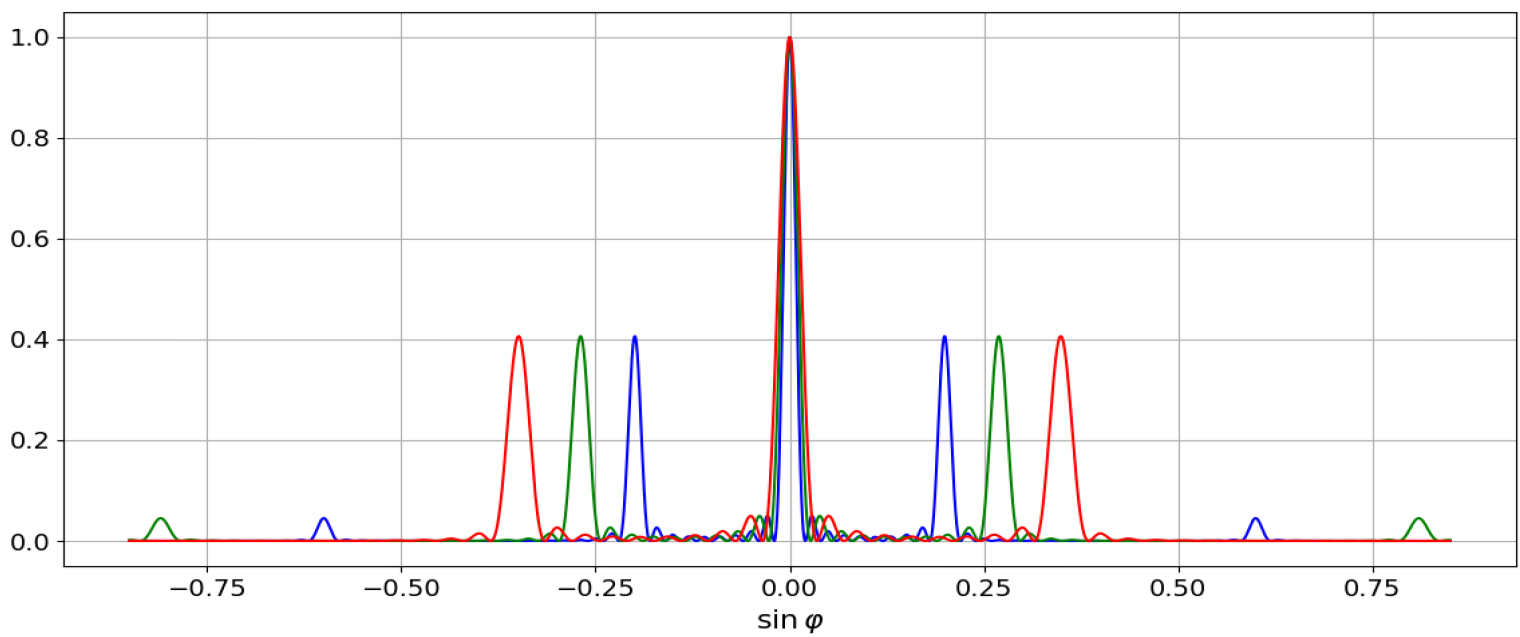
\includegraphics[width=0.9\columnwidth]{images/aufloesungsvermoegen.png}
\end{center}


\paragraph{Kriterium}


Zwei Wellenlängen werden gerade noch aufgelöst, wenn das Hauptmaximum von $\lambda_2$ mit dem Minimum von $\lambda_1$ zusammenfällt

$$ \boxed{ \frac{\lambda}{\Delta \lambda} = n \, Z } $$

\renewcommand{\arraystretch}{1.3}
\begin{ctabular}{clc}
    $\lambda$           & Wellenlänge                   & $[\lambda] = \meter$          \\
    $\Delta \lambda$    & Unterschied der Wellenlängen  & $[ \Delta \lambda] = \meter$  \\
    $n$                 & Ordnung der Beugung (typ. 1)  & $[n] = 1$                     \\
    $Z$                 & Anzahl der Spalten            & $[Z] = 1$ 
\end{ctabular}
\renewcommand{\arraystretch}{1}


\subsection{Babinet-Prinzip}

\begin{minipage}[t]{0.48\columnwidth}
    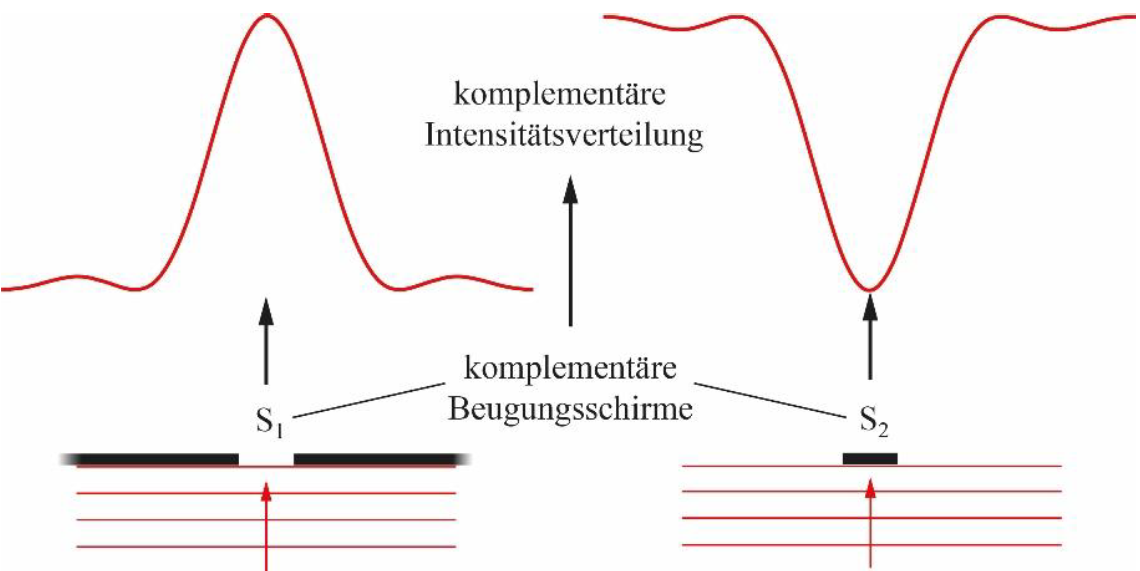
\includegraphics[width=\columnwidth, align=t]{images/babinet_prinzip.png}
\end{minipage}
\hfill
\begin{minipage}[t]{0.48\columnwidth}
    \raggedright%
    Ausserhalb des Bereichs geometrisch-optischer Abbildung produzieren komplementäre Beugungsschirme gleiche Beugungsbilder
\end{minipage}


        \section{Akustik}

\subsection{Teminologie}

\paragraph{Ton}

Eine harmonische Schallwelle wird als \textbf{Ton} bezeichnet.

Ein (reiner) Ton entspricht also einer \textbf{Schallschwingung}, die \textbf{eine einzige Frequenz} enthält.

\medskip
\paragraph{Klang}

Eine \textbf{Überlagerung} von harmonischen Schwingungen, deren \textbf{Frequenzen} in einem 
\textbf{ganzzahligen Verhältnis} zur tiefsten Frequenz, zur Frequenz des \textbf{Grundtons}, stehen, wird \textbf{Klang} genannt. 

\medskip
\paragraph{Geräusch}

Bei einem \textbf{Geräusch} besteht das Frequenzspektrum nicht mehr aus einzelnen diskreten Linien, sondern weist in einem bestimmten Frequenzbereich eine  \textbf{kontinuierliche Verteilung} auf.


\subsection{Pegel}

\begin{minipage}[t]{0.48\columnwidth}
    \paragraph{'Einheit': Bel}

    $$ \boxed{ \text{Pegel} = \log \left( \frac{x}{b_0} \right) } $$
    $$ \boxed{ x = b_0 \cdot 10^{\text{Pegel} } } $$ 
\end{minipage}
\hfill
\begin{minipage}[t]{0.48\columnwidth}
    \paragraph{'Einheit': Dezibel}

    $$ \boxed{ \text{Pegel} = 10 \cdot \log \left( \frac{x}{b_0} \right) } $$ 
    $$ \boxed{ x = b_0 \cdot 10^{\left( \frac{\text{Pegel}}{10} \right) } } $$
\end{minipage}

\renewcommand{\arraystretch}{1.3}
\begin{ctabular}{clc}
    Pegel   & Dimensionslose Grösse     & $[\text{Pegel}] =  1$ \\
    $x$     & Zu vergleichende Grösse   & $[x]$                 \\
    $b_0$   & Basisgrösse               & $[b_0] = [x]$
\end{ctabular}
\renewcommand{\arraystretch}{1}


\subsection{Schallintensität}

\begin{minipage}{0.48\columnwidth}
    $$ \boxed{ L_I = 10 \cdot \log \left( \frac{I}{I_0} \right) } $$ 
\end{minipage}
\hfill
\begin{minipage}{0.48\columnwidth}
    $$ \boxed{ L_p = 20 \cdot \log \left( \frac{p_{\rm eff}}{p_{\rm eff0}} \right) } $$ 
\end{minipage}

$$ \boxed{ p_{\rm eff} = \frac{\Delta p_0}{\sqrt{2}} } $$

\renewcommand{\arraystretch}{1.3}
\begin{ctabular}{clc}
    $L_I$           & Schallintensitätspegel        & $[L_I] = \deci\bel$                   \\
    $L_p$           & Schalldruckpegel              & $[L_p] = \deci\bel$                   \\
    $I$             & Intensität                    & $[I] = \frac{\watt}{\meter\squared}$  \\
    $p_{\rm eff}$   & Schalldruck (Effektivwert)    & $[p_{\rm eff}] = \pascal$             \\
    $\Delta p_0$    & Druckamplitude                & $[\Delta p_0] = \pascal$ 
\end{ctabular}

\begin{ctabular}{cll}
    $I_0$           & Bezugsintensität  & $I_0 = 10^{-12} \, \frac{\watt}{\meter\squared}$ \\
    $p_{\rm eff0}$  & Bezugsschalldruck & $p_{\rm eff0} = 2 \cdot 10^{-5} \pascal$
\end{ctabular}
\renewcommand{\arraystretch}{1}



\subsection{Intensität bei Kugelwellen}

\vspace{-0.4cm}

\renewcommand{\arraystretch}{3}
\begin{tabular}{@{}lll@{}}
					 & \textbf{ohne Dämpfung}                                               & \textbf{mit Dämpfung} \\
	Energieerhaltung & $\boxed{ I(r) = \frac{P}{4 \, \pi \, r^2} }$                         & $\boxed{ I(r) = \frac{P}{4 \, \pi \, r^2} \, \e^{- \alpha r}}$                       \\ 

	Verhältnis 		 & $\boxed{ \frac{I_2}{I_1} = \frac{r_1^2}{r_2^2} }$                    & $\boxed{ \frac{I_2}{I_1} = \frac{r_1^2}{r_2^2} \, \e^{- \alpha (r_2 - r_1)} }$        \\

	Pegel 			 & $\boxed{ L_2 = L_1 - 20 \cdot \log \left( \frac{r_2}{r_1} \right)}$  & $\boxed{ L_2 = L_1 - 20 \cdot \log \left( \frac{r_2}{r_1} \right) - K (r_2 - r_1)  }$ \\
\end{tabular}



\renewcommand{\arraystretch}{1.2}
\begin{ctabular}{clc}
	$I(r)$      & Intensität                                                            & $[I(r)] = \frac{\watt}{\meter\squared}$   \\
	$P$         & Leistung                                                              & $[P] = \watt$                             \\
	$r_i$       & Abstand (Radius) zum Wellenursprung                                   & $[r_i] = \meter\squared$                  \\
	$L_i$       & Pegel                                                                 & $[L_i] = \deci\bel$                       \\
	$\alpha$    & Absorptionsgrad ($\alpha = 1-R$, siehe \ref{Reflexion} )              & $[\alpha] = 1$                            \\
	$K$         & Dämpfung                                                              & $[K] = \frac{\deci\bel}{\meter}$
\end{ctabular}
\renewcommand{\arraystretch}{1}



\subsection{Verschiedene Schallquellen}

\begin{center}
    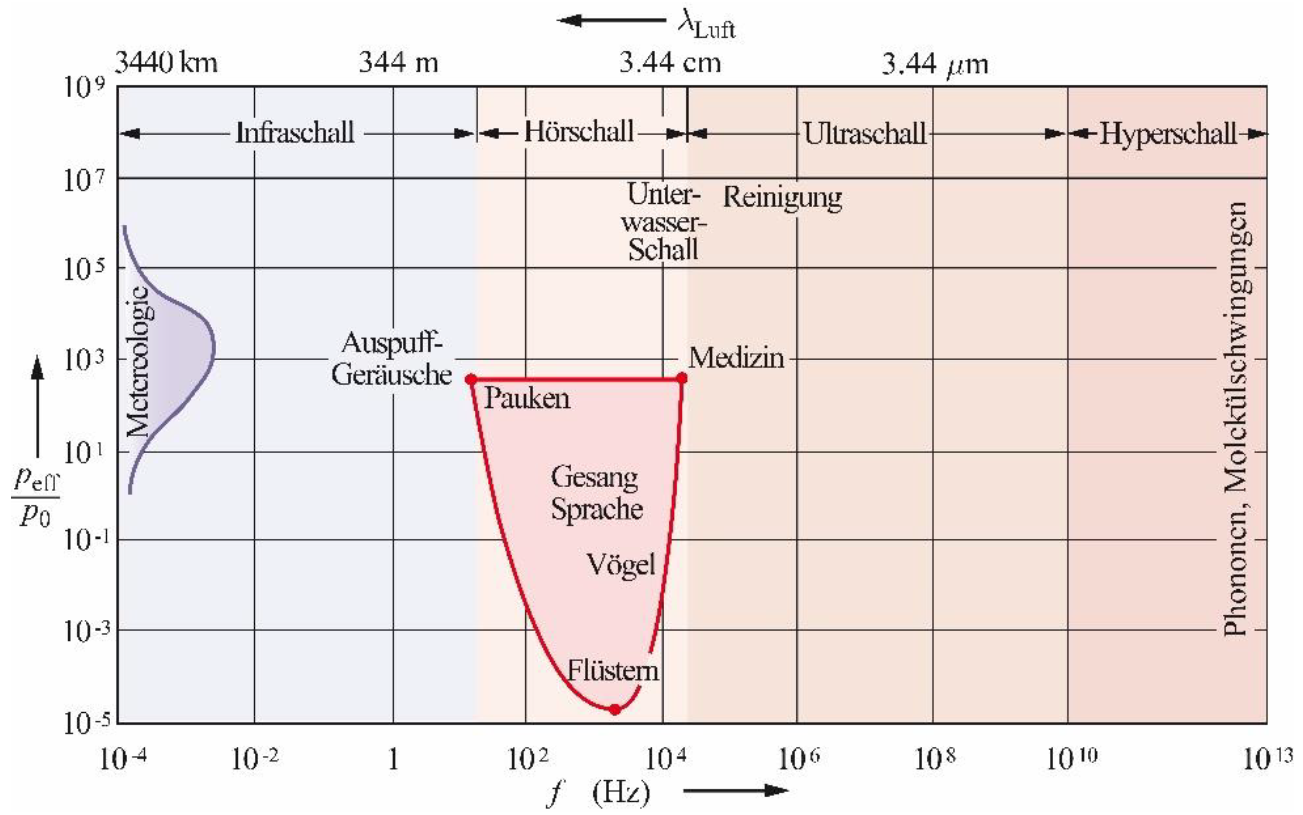
\includegraphics[width=0.9\columnwidth]{images/schallquellen.png}
\end{center}


\subsection{PHON-Skala}

\begin{center}
    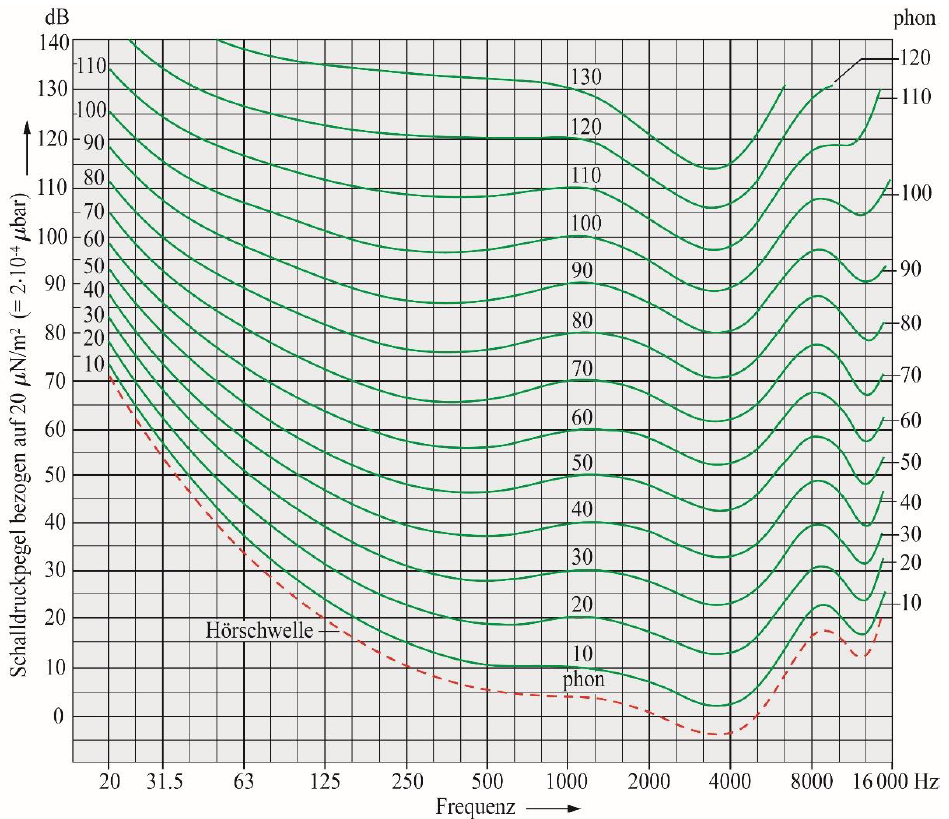
\includegraphics[width=\columnwidth]{images/phon_skala.png}
\end{center}



\subsection{Schalldämpfung / Schalldämmung}

\subsubsection{Schalldämpfung}

Schalldämpfung bedeutet eine \textbf{Abschwächung} der Schallwellen durch \textbf{Absorption}. 

Schallenergie wird in \textbf{'Wärme' umgewandelt}, d.h. durch die Absorption von Energie werden das von den Schallwellen
durchdrungene Medium oder die das Schallfeld begrenzenden Körper \textbf{erwärmt}.

\medskip
\paragraph{Verschiedene Arten von Absorption für Schalldämpfung Innen}

\begin{itemize}
	\item Poröse Schicht (mit oder ohne perforierte Abdeckung) 
	\item Akustikplatte 
	\item Plattenresonator
	\item Helmholtz-Resonator
\end{itemize}


\subsubsection{Schalldämmung} 

Schalldämmung ist die \textbf{Behinderung der Schallausbreitung} durch \textbf{reflektierende} Hindernisse. 
Mauern, Türen und Fenster bewirken eine Schalldämmung für den von aussen in das Gebäude eindringenden Schall. 
Auch die Ausbreitung von Schall innerhalb eines Gebäudes wird durch die Schalldämmung von Zwischenwänden und Türen abgeschwächt. 
Im Freien wird durch Schallschutzwände eine Schalldämmung für die dahinterliegenden Gebäude erreicht.


\subsection{Schalldämmung / Schalldämm-Mass}

Bei der Schallübertragung muss zwischen \textbf{Luftschall} und \textbf{Körperschall} unterschieden werden.


\subsubsection{Luftschalldämmung}

Es gibt Schallquellen, die ihre Schallenergie (fast) ausschliesslich in die Luft abstrahlen.

Beispiele: menschliche Stimme, Geigen, Lautsprecher und Blasinstrumente


\subsubsection{Körperschalldämmung}

Andere Schallerzeuger übertragen die Schallschwingungen nicht nur auf die Luft, sondern auch direkt auf feste Körper. 
Streichinstrumente, wie Cello oder Bassgeige, und Klavier oder Flügel übertragen die Schallschwingungen auch direkt auf den Fussboden. 
Wird ein Nagel in die Wand geschlagen, so wird ein grosser Anteil des erzeugten Schalls als Körperschall übertragen.

Beispiele: Trittschall, Wasserleitungsgeräusche


\subsection{Schalldämm-Mass}

$$ \boxed{ \mathcal{R} = 10 \cdot \left( \frac{P_1}{P_2} \right)  } $$


\subsection{Anhall / Nachhall}

\subsubsection{Anhall}

Es dauert eine gewisse Zeit, bis sich eine \text{konstante Energiedichte} der Schallwellen \text{im Raum aufgebaut} hat. Dieser Vorgang wird Anhall genannt. Wegen der logarithmischen Empfindlichkeit des Ohrs \text{wird er praktisch nicht wahrgenommen}.


\subsubsection{Nachhall}

Die von den Begrenzungsflächen des Raumes mehrfach reflektierten Wellen bewirken andererseits, dass beim \text{plötzlichen Abschalten} einer Schallquelle der Schall nicht sofort verschwindet, sondern \text{allmählich abklingt}. Dieses Phänomen wird Nachhall genannt und ist im Gegensatz zum Anhall \text{deutlich wahrnehmbar}.

\medskip
\textbf{Per Definition ist die Nachhallzeit jene Zeitspanne, in welcher der Schallpegel im Raum um 60 dB sinkt.}


\subsubsection{Nachhallzeit $\bm{T_N}$}

$$ \boxed{ T_N = 0.16 \, \frac{\second}{\meter} \frac{V}{\sum\limits_i \alpha_i A_i } } $$

\renewcommand{\arraystretch}{1.3}
\begin{ctabular}{clc}
    $T_N$       & Nachhallzeit & $[T_N] = \second$ \\
    $V$         & Raumvolumen & $[V] = \meter\cubed$ \\
    $\alpha_i$  & Absoptionsgrad & $[\alpha_i] = 1$ \\
    $A_i$       & Teilfläche der Raumbegrenzung mit Absorption $\alpha_i$ & $[A_i] = \meter\squared$ \\ 
\end{ctabular}
\renewcommand{\arraystretch}{1}



        \columnbreak

        \part{Anhang}
		\section{Anhang}

\subsection{Massenträgheitsmomente}\label{Massenträgheitsmomente}

\begin{ctabular}{| c | c |}
  \hline
  \textbf{Zylinder / Scheibe}                                                 & \textbf{Hohlzylinder}                                                     \\
  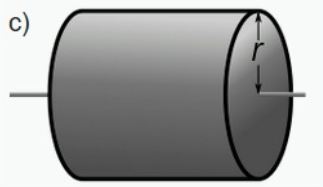
\includegraphics[width=0.35\columnwidth]{images/J_zylinder.png}             & 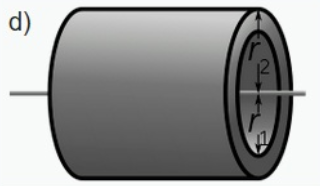
\includegraphics[width=0.35\columnwidth]{images/J_hohlzylinder.png}       \\
  $J = \frac{1}{2} m r^2$                                                     & $J = m \, \frac{r_1^2 + r_2^2}{2}$                                        \\
  \hline
  \textbf{Dünner Stab (Mitte)}                                                & \textbf{Dünner Stab (Ende)}                                               \\
  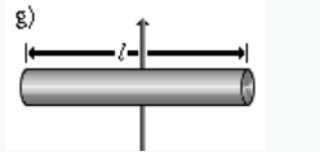
\includegraphics[width=0.35\columnwidth]{images/J_duenner_stab_mitte.png}   & 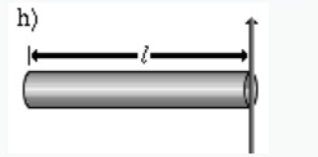
\includegraphics[width=0.35\columnwidth]{images/J_duenner_stab_ende.png}  \\
  $J = \frac{1}{12} m l^2$                                                    & $J = \frac{1}{3} m l^2$                                                   \\
  \hline
  \textbf{Kugel}                                                              & \textbf{Massenpunkt}                                                      \\
  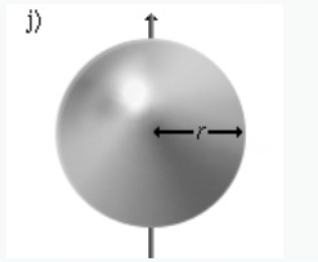
\includegraphics[width=0.35\columnwidth]{images/J_kugel.png}                & 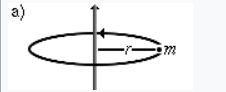
\includegraphics[width=0.35\columnwidth]{images/J_massepunkt.png}         \\
  $J = \frac{2}{5} m r^2$                                                     & $J = m r^2$                                                               \\
  \hline
\end{ctabular}

\subsection{Messunsicherheit \& geltende Stellen}

\[
  \Delta y = \sqrt{\sum_{i} \left( \frac{\partial y}{\partial x_i} \right)^2 \cdot \Delta x_i^2}
\]

\begin{ctabular}{| c | c | c | c |}
  \hline
  \textbf{Unsicherheit} & \textbf{Führende Ziffer} & \textbf{Gerundete Unsicherheit} & \textbf{Nachkommastellen} \\
  \hline
  0.30 & 3 & 0.3 & 1 \\
  0.25 & 2 & 0.25 & 2 \\
  0.002 & 2 & 0.0020 & 4 \\
  0.005 & 5 & 0.005 & 3 \\
  \hline
\end{ctabular}

\begin{itemize}
  \item Unsicherheit: 1--2 geltende Stellen (zwei nur bei führender 1 oder 2).
  \item Messwert: letzte Ziffer auf derselben Dezimalstelle wie die letzte Ziffer der Unsicherheit.
\end{itemize}

\subsection{Trigonometrie}

\begingroup
\renewcommand{\arraystretch}{2}
\setlength{\tabcolsep}{0mm}
\scalebox{0.33}{
  \Huge
  \begin{tabularx}{3\columnwidth}{rp{1mm}V{3}*{17}{C}}
    \rowcolor{subsectioncolor!30}$\bm{\alpha}$\phantom{${}^{\circ}$} && $0$ & $\dfrac{\pi}{6\mathstrut}$ & $\dfrac{\pi}{4}$ & $\dfrac{\pi}{3}$ & $\dfrac{\pi}{2}$ & $\dfrac{2\pi}{3}$ & $\dfrac{3\pi}{4}$ & $\dfrac{5\pi}{6}$ & $\pi$ & $\dfrac{7\pi}{6}$ & $\dfrac{5\pi}{4}$ & $\dfrac{4\pi}{3}$ & $\dfrac{3\pi}{2}$ & $\dfrac{5\pi}{3}$ & $\dfrac{7\pi}{4}$ & $\dfrac{11\pi}{6}$ & $2\pi$ \\\hline
    \rowcolor{subsectioncolor!30}$\bm{\alpha^\circ}$ && \phantom{${}^\circ$}$0^\circ$ & $30^\circ$ & $45^\circ$ & $60^\circ$ & $90^\circ$ & $120^\circ$ & $135^\circ$ & $150^\circ$ & $180^\circ$ & $210^\circ$ & $225^\circ$ & $240^\circ$ & $270^\circ$ & $300^\circ$ & $315^\circ$ & $330^\circ$ & $360^\circ$ \\\hline
    $\bm{\sin(\alpha)}$ && $0$ & $\dfrac{1}{2\mathstrut}$ & $\dfrac{\sqrt{2}}{2}$ & $\dfrac{\sqrt{3}}{2}$ & $1$ & $\dfrac{\sqrt{3}}{2}$ & $\dfrac{\sqrt{2}}{2}$ & $\dfrac{1}{2}$ & $0$ & $-\dfrac{1}{2}$ & $-\dfrac{\sqrt{2}}{2}$ & $-\dfrac{\sqrt{3}}{2}$ & $-1$ & $-\dfrac{\sqrt{3}}{2}$ & $-\dfrac{\sqrt{2}}{2}$ & $-\dfrac{1}{2}$ & $0$ \\\hline
    $\bm{\cos(\alpha)}$ && $1$ & $\dfrac{\sqrt{3}}{2\mathstrut}$ & $\dfrac{\sqrt{2}}{2}$ & $\dfrac{1}{2}$ & $0$ & $-\dfrac{1}{2}$ & $-\dfrac{\sqrt{2}}{2}$ & $-\dfrac{\sqrt{3}}{2}$ & $-1$ & $-\dfrac{\sqrt{3}}{2}$ & $-\dfrac{\sqrt{2}}{2}$ & $-\dfrac{1}{2}$ & $0$ & $\dfrac{1}{2}$ & $\dfrac{\sqrt{2}}{2}$ & $\dfrac{\sqrt{3}}{2}$ & $1$ \\\hline
    $\bm{\tan(\alpha)}$ && $0$ & $\dfrac{\sqrt{3}}{3\mathstrut}$ & $1$ & $\sqrt{3}$ & $\pm\infty$ & $-\sqrt{3}$ & $-1$ & $-\dfrac{\sqrt{3}}{3}$ & $0$ & $\dfrac{\sqrt{3}}{3}$ & $1$ & $\sqrt{3}$ & $\pm\infty$ & $-\sqrt{3}$ & $-1$ & $-\dfrac{\sqrt{3}}{3}$ & $0$ \\\hline
    $\bm{\cot(\alpha)}$ && $\pm\infty$ & $\sqrt{3}$ & $1$ & $\dfrac{\sqrt{3}}{3\mathstrut}$ & $0$ & $-\dfrac{\sqrt{3}}{3}$ & $-1$ & $-\sqrt{3}$ & $\pm\infty$ & $\sqrt{3}$ & $1$ & $\dfrac{\sqrt{3}}{3}$ & $0$ & $-\dfrac{\sqrt{3}}{3}$ & $-1$ & $-\sqrt{3}$ & $\pm\infty$ \\
\end{tabularx}}
\endgroup

\subsubsection{Beziehungen zwischen $\bm{\sin(x)}$ und $\bm{\cos(x)$}}

\begin{tabular}{lll}
  $\sin(-a) = -\sin(a)$   & $\sin(\pi - a) = \sin(a)$     & $\sin(\pi + a) = -\sin(a)$ \\
  $\cos(-a) = \cos(a)$    & $\cos(\pi - a) = - \cos(a)$   & $\cos(\pi + a) = - \cos(a)$ \\
  \\
\end{tabular}

\begin{tabular}{ll}
  $\sin(\frac{\pi}{2} - a) = \sin(\frac{\pi}{2} + a) = \cos(a)$ & $\cos(\frac{\pi}{2} - a) = - \cos(\frac{\pi}{2} + a) = \sin(a)$
\end{tabular}

\subsubsection{Additionstheoreme}

\begin{tabular}{ll}
  $\sin(a \pm b) = \sin(a) \cdot \cos(b) \pm \cos(a) \cdot \sin(b)$   & $\tan(a \pm b) = \frac{\tan(a) \pm \tan(b)}{1 \mp \tan(a) \cdot \tan(b)}$\\
  $\cos(a \pm b) = \cos(a) \cdot \cos(b) \mp \sin(a) \cdot \sin(b)$   &
\end{tabular}

\subsubsection{Summen und Differenzen}

\renewcommand{\arraystretch}{1.5}
\begin{tabular}{ll@{}}
  $\sin(a) + \sin(b) = 2 \cdot \sin \big( \frac{a+b}{2} \big) \cdot \cos \big( \frac{a-b}{2} \big)$ &
  $\cos(a) + \cos(b) = 2 \cdot \cos \big( \frac{a+b}{2} \big) \cdot \cos \big( \frac{a-b}{2} \big)$ \\
  $\sin(a) - \sin(b) = 2 \cdot \sin \big( \frac{a-b}{2} \big) \cdot \cos \big( \frac{a+b}{2} \big)$ &
  $\cos(a) - \cos(b) = -2 \cdot \sin \big( \frac{a+b}{2} \big) \cdot \sin \big( \frac{a-b}{2} \big)$ \\
  $\tan(a) \pm \tan(b) = \frac{\sin(a \pm b)}{\cos(a) \cdot \cos(b)}$
\end{tabular}
\renewcommand{\arraystretch}{1}

\subsubsection{Produkte}

$\sin(a) \cdot \sin(b) = \frac{1}{2} \big( \cos(a-b) - \cos(a+b) \big) $ \\
$\cos(a) \cdot \cos(b) = \frac{1}{2} \big( \cos(a-b) + \cos(a+b) \big) $ \\
$\sin(a) \cdot \cos(b) = \frac{1}{2} \big( \sin(a-b) + \sin(a+b) \big) $


\subsubsection{Winkelvielfache und Halbwinkel}

\renewcommand{\arraystretch}{1.3}
\begin{tabular}{ll}
  $\sin(2a) = 2 \, \sin(a) \cdot \cos(a)$                         & $\cos(2a) = \cos^2(a) - \sin^2(a)$                                \\
  $\sin(3a) = 3 \, \sin(a) -4 \, \sin^3(a)$                       & $\cos(3a) = 4 \, \cos^3(a) -3 \, \cos(a)$                         \\
  $\sin \big( \frac{a}{2} \big) = \sqrt{\frac{1}{2}(1-\cos(a))} $ & $\cos \big( \frac{a}{2} \big) = \sqrt{\frac{1}{2}(1+\cos(a))} $
\end{tabular}

\subsubsection{Potenzen}

\renewcommand{\arraystretch}{1.5}
\begin{tabular}{ll}
  $\sin^2(a) = \frac{1^{\mathstrut}}{2}(1-\cos(2a))$               & $\cos^2(a) = \frac{1}{2}(1+\cos(2a))$                \\
  $\sin^3(a) = \frac{1^{\mathstrut}}{4}(3\, \sin(a) - \sin(3a))$   & $\cos^3(a) = \frac{1}{4}(\cos(3a) + 3 \, \cos(a))$
\end{tabular}
\renewcommand{\arraystretch}{1}

    \end{layout}
\end{document}
